\documentclass[11pt]{article}
\usepackage[top=2cm,left=2cm,right=2cm,bottom=2cm]{geometry}
\usepackage[doublespacing]{setspace}
\usepackage{graphicx}
\usepackage{xcolor}
\usepackage{subfigure}
\usepackage[hidelinks]{hyperref}
\usepackage{amsmath}
\usepackage{amssymb}
\usepackage{lscape}
\usepackage{booktabs}
\usepackage[localise]{xepersian}
\settextfont{XB Niloofar}


\begin{document}
	\شروع{وسط‌چین}
	به نام خدا\\
	\vspace{1cm}
	\begin{figure}[h]
		\begin{center}
			\includegraphics[width=0.3\linewidth]{"D:/Logo/UT"}
		\end{center}
	\end{figure}
	{\درشت‌درشت دانشکده مهندسی مکانیک}\\
	\vspace{1cm}
	{\بزرگ \سیاه{نام درس: هوش مصنوعی}}\\
	
	\vspace{0.5cm}
	{\درشت‌درشت تمرین ۲(یادگیری ماشین)}
	\vspace{1.5cm}
	
	\vspace{1.5cm}
	{\درشت‌درشت {\سیاه استاد درس:} دکتر شریعت‌پناهی}\\
	\vspace{2cm}
	{\درشت‌درشت {\سیاه دانشجو:}}\\
	{\درشت مهدی نوذری\\
	810601139}\\
	\vspace{3cm}
	بهار ۱۴۰۳\\
	\پایان{وسط‌چین}
	\pagebreak
	تمامی فایل‌ها در \lr{Github} موجود هستند:
	\href{https://github.com/Morphit/UT_AI_1403}{\lr{https://github.com/Morphit/UT\_AI\_1403}}
	\section{بخش اول: رگرسیون}
	در این بخش طراحی و تربیت مدلی انجام می‌شود که بر اساس ۲۴ ویژگی خودرو، قیمت آن را پیش بینی می‌کند.
	\subsection{بررسی دادگان خام}
	با استفاده از دستور 
	\verb|df.info()|
	اطلاعات و ساختار کلی داده‌ها به دست می‌آید که در 
	\autoref{tab:dataframe_info1}
	نشان داده شده اند.
	\begin{table}[h!]
		\centering
		\caption{ساختار کلی داده‌ها}
		\begin{latin}
		{\scriptsize
		\begin{tabular}{cccc}
				\toprule
				\# & Column             & Non-Null Count & Dtype   \\ 
				\midrule
				0  & car\_ID            & 205 non-null   & int64   \\ 
				1  & symboling          & 205 non-null   & int64   \\ 
				2  & CarName            & 205 non-null   & object  \\ 
				3  & fueltype           & 205 non-null   & object  \\ 
				4  & aspiration         & 205 non-null   & object  \\ 
				5  & doornumber         & 205 non-null   & object  \\ 
				6  & carbody            & 205 non-null   & object  \\ 
				7  & drivewheel         & 205 non-null   & object  \\ 
				8  & enginelocation     & 205 non-null   & object  \\ 
				9  & wheelbase          & 205 non-null   & float64 \\ 
				10 & carlength          & 205 non-null   & float64 \\ 
				11 & carwidth           & 205 non-null   & float64 \\ 
				12 & carheight          & 205 non-null   & float64 \\ 
				13 & curbweight         & 205 non-null   & int64   \\ 
				14 & enginetype         & 205 non-null   & object  \\ 
				15 & cylindernumber     & 205 non-null   & object  \\ 
				16 & enginesize         & 205 non-null   & int64   \\ 
				17 & fuelsystem         & 205 non-null   & object  \\ 
				18 & boreratio          & 205 non-null   & float64 \\ 
				19 & stroke             & 205 non-null   & float64 \\ 
				20 & compressionratio   & 205 non-null   & float64 \\ 
				21 & horsepower         & 205 non-null   & int64   \\ 
				22 & peakrpm            & 205 non-null   & int64   \\ 
				23 & citympg            & 205 non-null   & int64   \\ 
				24 & highwaympg         & 205 non-null   & int64   \\ 
				25 & price              & 205 non-null   & float64 \\ 
				\bottomrule
		\end{tabular}
		}
		\end{latin}
		\label{tab:dataframe_info1}
	\end{table}
	همچنین در
	\autoref{tab:stats_1}
	اطلاعات آماری ویژگی‌هایی که با اعداد توصیف می‌شوند شامل مقادیر کمینه، بیشینه و انحراف معیار قابل مشاهده است.
	\begin{table}[h!]
		\centering
		\caption{مقادیر آماری داده‌های عددی}
		\begin{latin}
			{\scriptsize
		\begin{tabular}{lccc}
			\toprule
			Feature           & Max     & Min     & Std    \\ 
			\midrule
			wheelbase         & 120.90  & 86.60    & 3.626178e+01   \\ 
			carlength         & 208.10  & 141.10    & 1.522087e+02   \\ 
			carwidth          & 72.30   & 60.30    & 4.601900e+00   \\ 
			carheight         & 59.80   & 47.80    & 5.970800e+00   \\ 
			curbweight        & 4066.00 & 1488.00    & 2.711079e+05   \\ 
			enginesize        & 326.00  & 61.00    & 1.734114e+03   \\ 
			boreratio         & 3.94    & 2.54    & 7.335631e-02   \\ 
			stroke            & 4.17    & 2.07	  & 9.834309e-02   \\ 
			compressionratio  & 23.00   & 7.00    & 1.577710e+01   \\ 
			horsepower        & 288.00  & 48.00    & 1.563741e+03   \\ 
			peakrpm           & 6600.00 & 4150.00    & 2.275153e+05   \\ 
			citympg           & 49.00   & 13.00    & 4.279962e+01   \\ 
			highwaympg        & 54.00   & 16.00    & 4.742310e+01   \\ 
			price             & 45400.00& 5118.00    & 6.382176e+07   \\ 
			\bottomrule
		\end{tabular}
		}
		\end{latin}
		\label{tab:stats_1}
	\end{table}
	به منظور درک وابستگی ویژگی‌ها با یکدیگر، نمودار 
	\lr{correlation}
	را می‌توان در 
	\autoref{fig:correlation1}
	دید.
	\begin{figure}[!h]
		\centerline{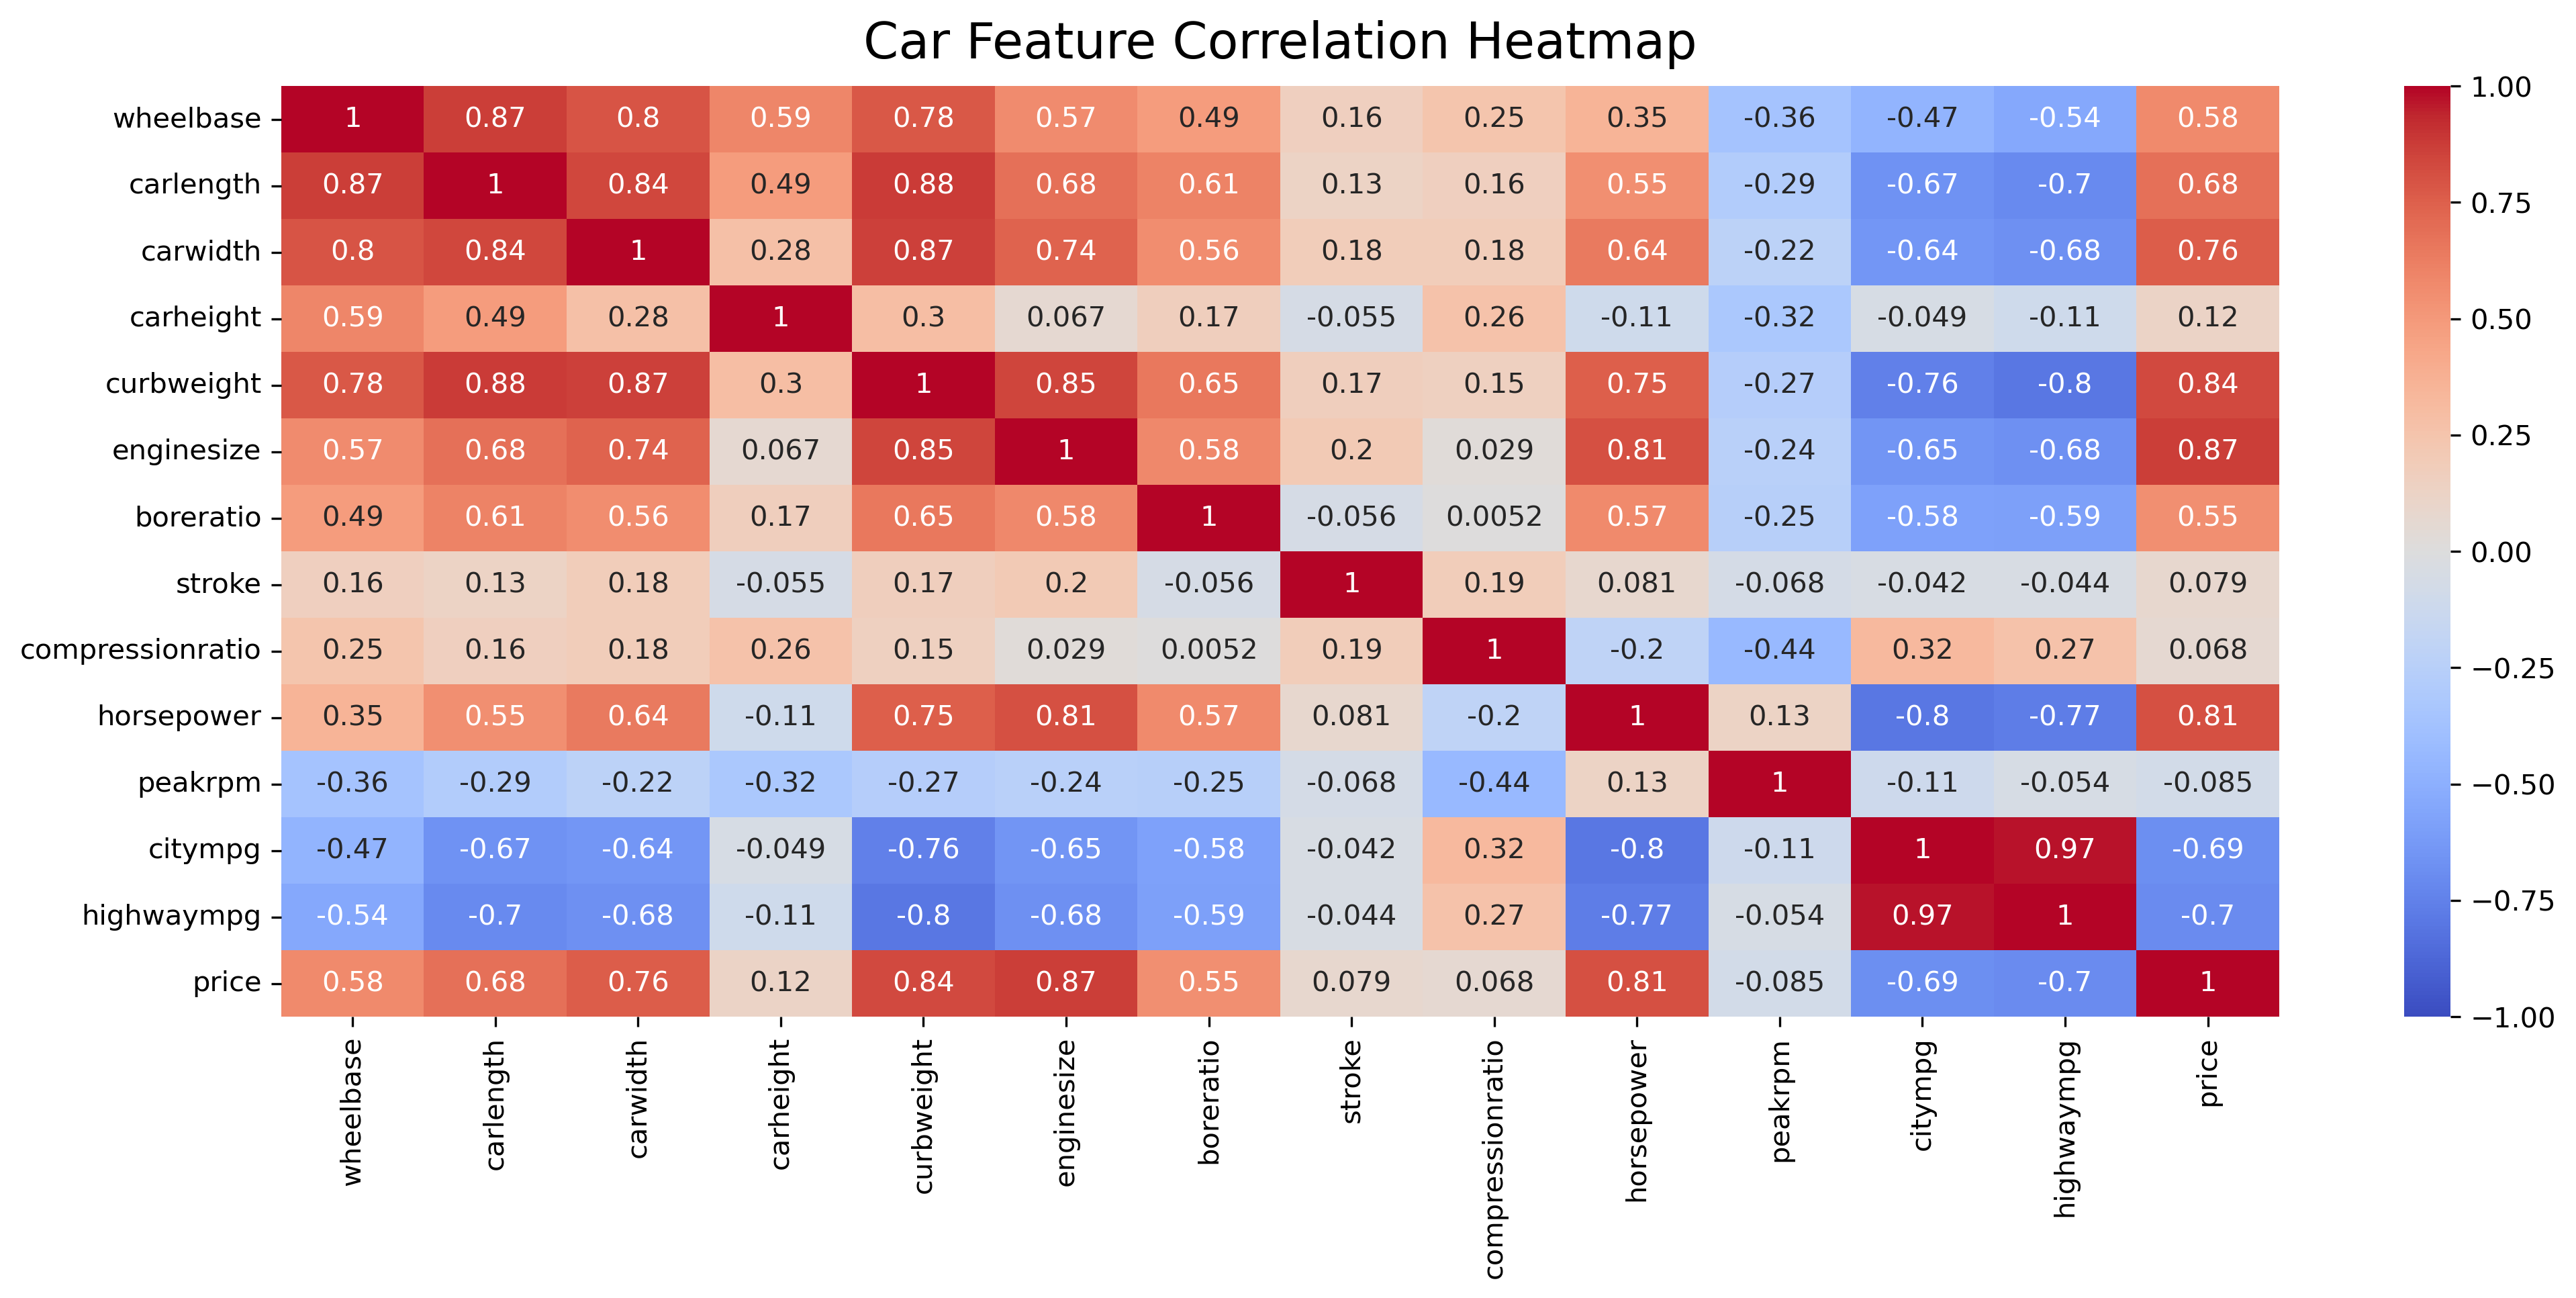
\includegraphics[width=1\linewidth]{../HW2_1/CorrelationHeatmap.png}}
		\caption{نمودار وابستگی داده‌ها}
		\label{fig:correlation1}
	\end{figure}
	\subsection{پیش پردازش دادگان}
	به منظور جداسازی داده‌های آموزش و آزمون با استفاده از 
	\verb|test_train_split|
	۷۰ درصد داده‌ها برای آموزش و باقی برای آزمون جدا شدند. بنابراین ۱۴۳ داده برای آموزش و ۶۲ داده مخصوص آزمون هستند.\\
	\autoref{fig:jointplot}
	نشان‌دهنده ارتباط بین دو ویژگی \lr{horsepower} و \lr{enginesize} می‌باشد. از این نمودار می‌توان دریافت که این داده ‌ها تقریبا رابطه خطی مستقیم با یک‌دیگر دارند. به این ترتیب با افزایش حجم موتور، توان افزایش می‌یابد که امری منطقیست.
	 \begin{figure}[!h]
	 	\centerline{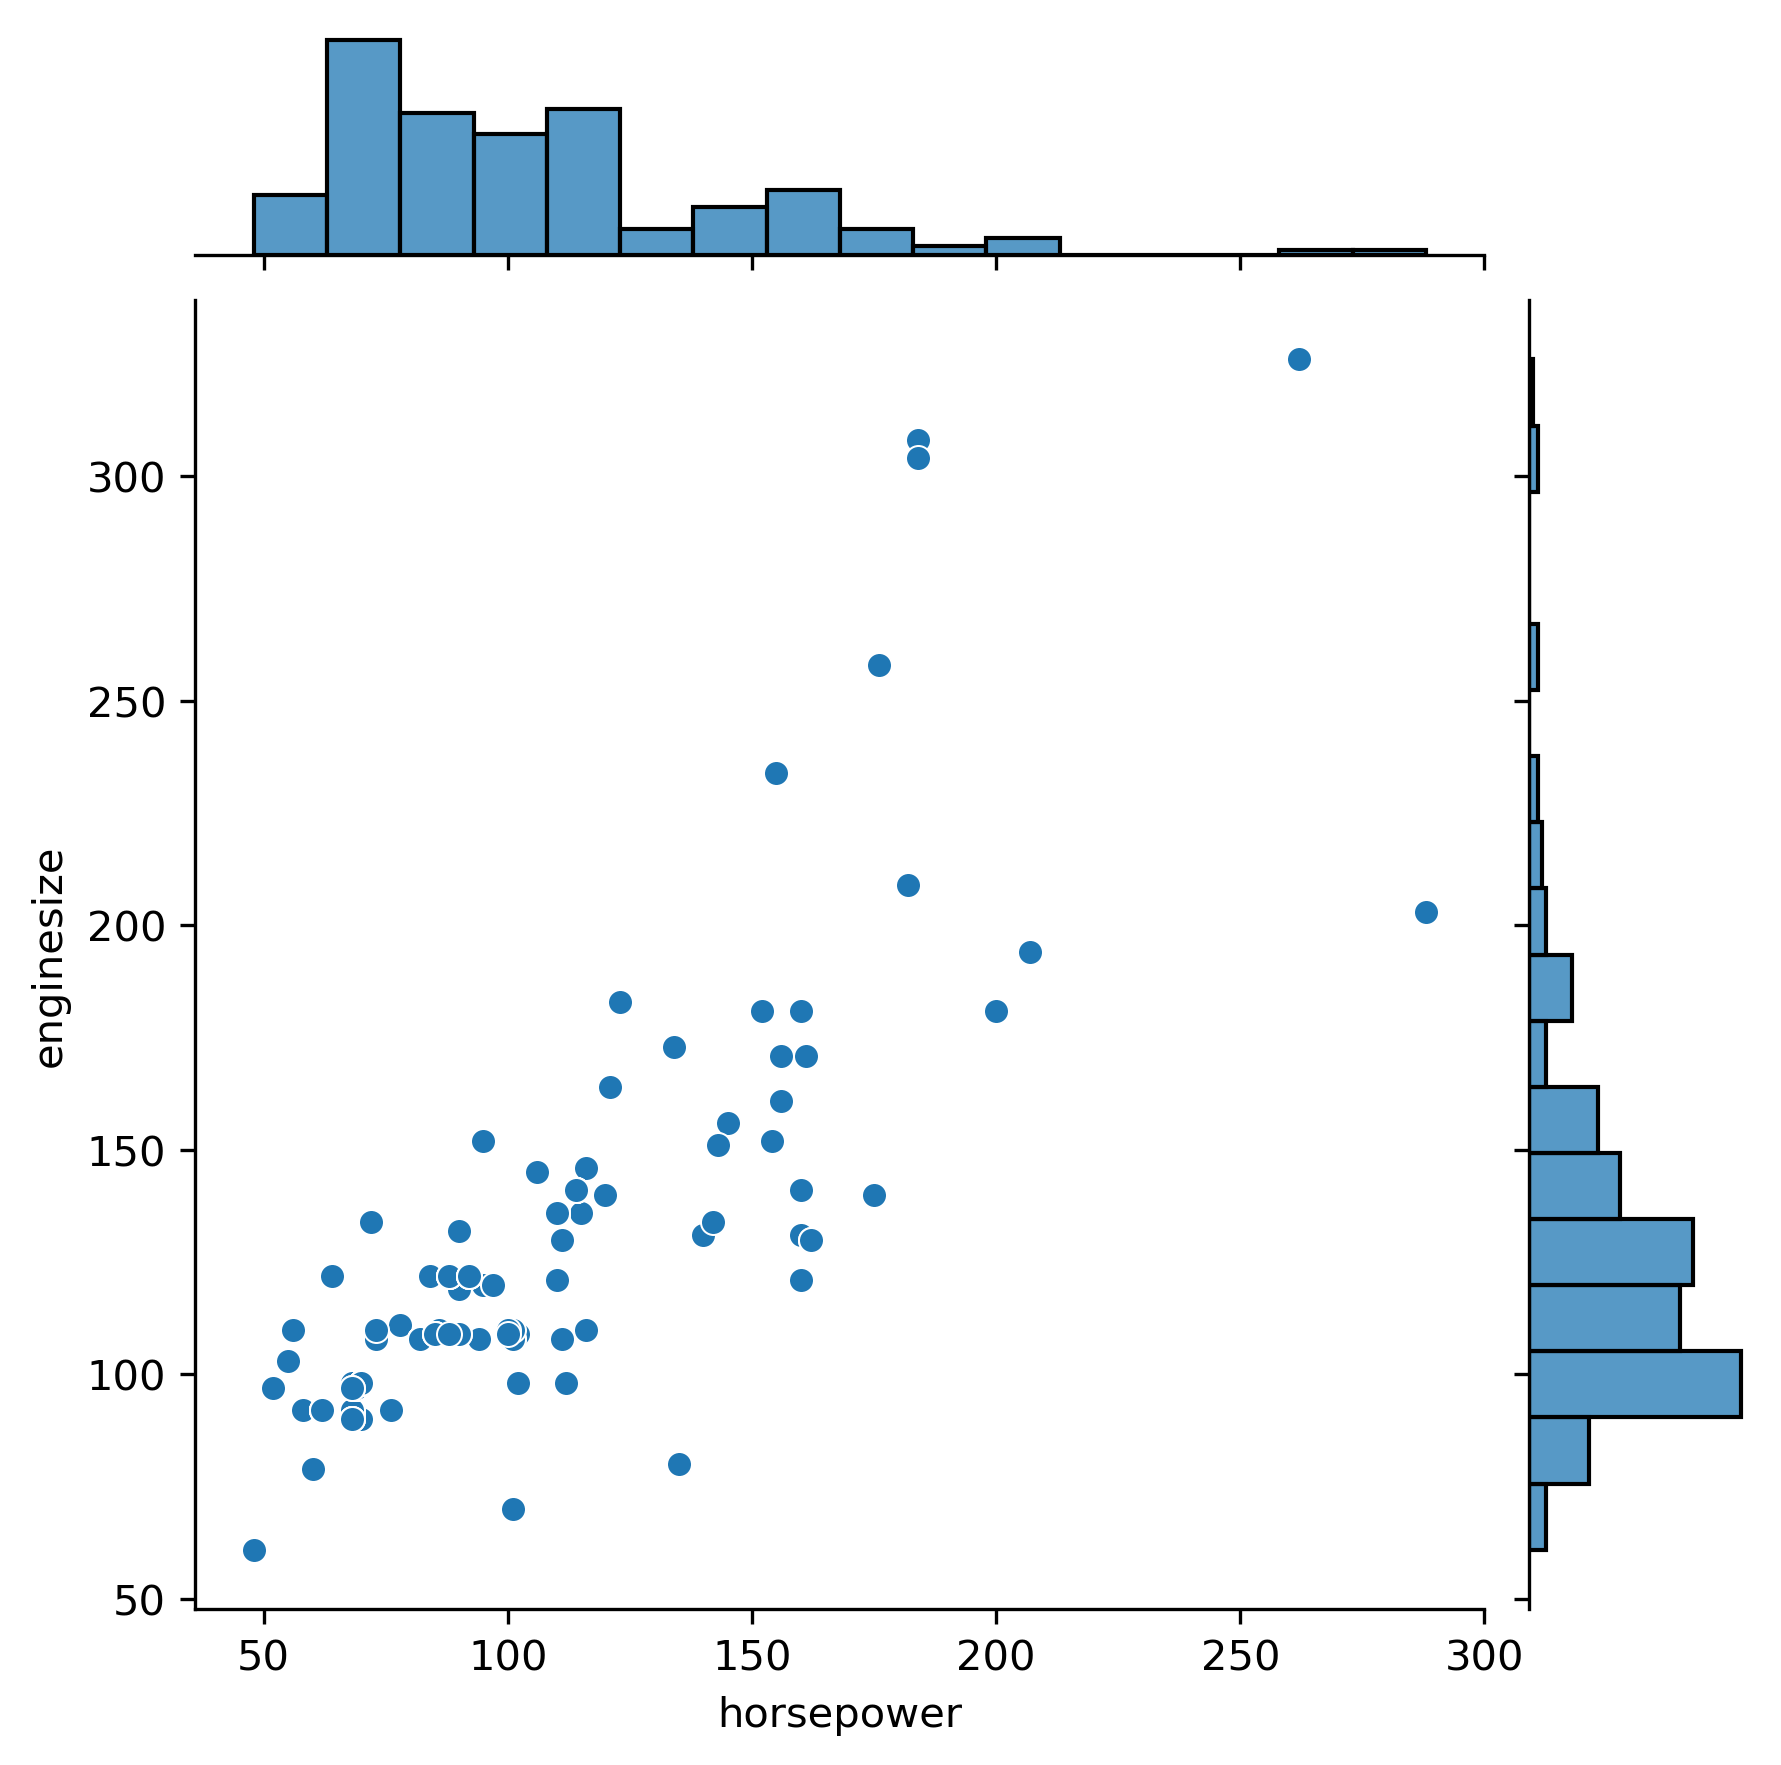
\includegraphics[width=0.6\linewidth]{../HW2_1/Jointplot.png}}
	 	\caption{نمودار ارتباط دو ویژگی \lr{horsepower} و \lr{enginesize}}
	 	\label{fig:jointplot}
	 \end{figure}\\
	 به منظور جداسازی ویژگی‌های موثر تر در تعیین قیمت خودرو،‌
	 \verb|SelectKBest|
	 می‌توان ۱۰ ویژگی موثرتر را انتخاب نمود. معیار
	 \verb|f_regression|
	 به دلیل اینکه در نهایت مدل رگرسیون است انتخاب می‌شود.
	 
	\subsection{انتخاب، آموزش و ارزیابی مدل}
	برای ارزیابی مدل دو معیار زیر در نظر گرفته می‌شوند.
	\begin{enumerate}
		\item \lr{RSME} $$RSME = \sqrt{\sum_{i=1}^{n}\frac{(\hat{y}_i^2 - y_i)^2}{n}}$$
		در این رابطه عبارت داخل پرانتز همان خطای پیش‌بینی مقدار می‌باشد.
		\item \lr{$R^2$score} $$R^2= 1 - \frac{\sum_{i=1}^{n}(y_i - \hat{y}_i)^2}{\sum_{i=1}^{n}(y_i - \bar{y}_i)^2}$$
		در این رابطه عبارت روی کسر خطای پیش‌بینی و $\bar{y}$ میانگین داده‌هاست.
	\end{enumerate}
	\begin{table}[h!]
		\caption{دقت مدل‌های آموزش داده شده}
		\begin{latin}
		\centering
		\begin{tabular}{|l|c|c|c|}
			\hline
			\textbf{Model} & \textbf{Train R² Score} & \textbf{Test R² Score} & \textbf{Test RMSE} \\ \hline
			Linear Regression  & 0.866847 & 0.797497 & 3745.707 \\ \hline
			Lasso Regression & 0.866847 & 0.797495 & 3745.720 \\ \hline
			Ridge Regression & 0.866755 & 0.797754 & 3743.329 \\ \hline
			SVR ($C=20000$, $\epsilon = 1$) & 0.978306 & 0.840435 & 3324.956 \\ \hline
		\end{tabular}
		\end{latin}
		\label{tab:regression_results}
	\end{table}
		به طور کلی تفاوت قابل ملاحظه‌ای میان ۳ مدل اول دیده نمی‌شود. اما با تنظیم مناسب پارامتر همسان‌سازی $C$ در مدل SVR می‌توان به نسبت مدل‌های دیگر نتیجه مطلوب‌تری گرفت. در این مسئله مقدار $C$ با صحیح و خطا پیدا شده اما برای پیدا کردن مقدار $C$ بهینه در مدل می‌توان از 
	\verb|GridSearchCV|
	استفاده نمود.
	\section{بخش دوم: دسته‌بندی}
	در این قسمت یک مسئله دسته‌بندی وجود دارد که باید در نهایت مدلی آموزش داده شود که براساس ۸ ویژگی افراد مونث، داشتن دیابت را پیش‌بینی کند.
	\subsection{بررسی دادگان خام}
		با استفاده از دستور 
	\verb|df.info()|
	اطلاعات و ساختار کلی داده‌ها به دست می‌آید که در 
	\autoref{tab:dataframe_info2}
	نشان داده شده اند.
	\begin{table}[h!]
		\centering
		\caption{ساختار کلی داده‌ها}
		\begin{latin}
			{\scriptsize
				\begin{tabular}{cccc}
					\toprule
					\# & Column                     & Non-Null Count   & Dtype   \\ 
					\midrule
					0  & Pregnancies                & 635 non-null     & float64 \\ 
					1  & Glucose                    & 654 non-null     & float64 \\ 
					2  & BloodPressure              & 680 non-null     & float64 \\ 
					3  & SkinThickness              & 624 non-null     & float64 \\ 
					4  & Insulin                    & 680 non-null     & float64 \\ 
					5  & BMI                        & 684 non-null     & float64 \\ 
					6  & DiabetesPedigreeFunction   & 590 non-null     & float64 \\ 
					7  & Age                        & 655 non-null     & float64 \\ 
					8  & Outcome                    & 768 non-null     & int64   \\ 
					\bottomrule
				\end{tabular}
			}
		\end{latin}
		\label{tab:dataframe_info2}
	\end{table}
	
		با استفاده از دستور 
	\verb|df.describe()|
	اطلاعات آماری داده‌ها در 
	\autoref{tab:stats_2}
	نشان داده شده اند.
	\begin{table}[h!]
		\caption{اطلاعات به دست آمده از طریق روش \lr{describe}}
		\begin{latin}
		{\scriptsize
		\centering
		\begin{tabular}{lccccccccc}
			\toprule
		 & \textbf{Pregnancies} & \textbf{Glucose} & \textbf{BloodPressure} & \textbf{SkinThickness} & \textbf{Insulin} & \textbf{BMI} & \textbf{Diabetes} & \textbf{Age} & \textbf{Outcome}\\ 
		&  &  &  &  &  &  & \textbf{Pedigree Function} &  &  \\ 
		\midrule
		count & 635.00 & 654.00 & 680.00 & 624.00 & 680.00 & 684.00 & 590.00 & 655.00 & 768.00 \\ 
		mean & 3.70 & 113.42 & 68.79 & 20.39 & 80.12 & 32.08 & 0.47 & 33.16 & 0.35 \\ 
		std & 3.52 & 202.82 & 19.72 & 15.99 & 115.68 & 7.80 & 0.32 & 13.83 & 0.48 \\ 
		min & -22.00 & -5000.00 & -2.00 & 0.00 & 0.00 & 0.00 & 0.08 & -150.00 & 0.00 \\ 
		25\% & 1.00 & 99.00 & 62.00 & 0.00 & 0.00 & 27.38 & 0.24 & 24.00 & 0.00 \\ 
		50\% & 3.00 & 117.00 & 72.00 & 23.00 & 34.00 & 32.30 & 0.37 & 29.00 & 0.00 \\ 
		75\% & 6.00 & 140.75 & 80.00 & 32.00 & 129.25 & 36.60 & 0.61 & 41.00 & 1.00 \\ 
		max & 17.00 & 199.00 & 122.00 & 99.00 & 846.00 & 67.10 & 2.33 & 81.00 & 1.00 \\ 
			\bottomrule
		\end{tabular}
		}
		\end{latin}
		\label{tab:stats_2}
	\end{table}
	
	به منظور اصلاح داده‌های ناموجود، ابتدا تعداد داده‌های ناموجود را بررسی می‌کنیم که در 
	\autoref{tab:missing_values2}
	آمده‌ است.
	\begin{table}[h!]
				\centering
		\caption{تعداد مقادیر ناموجود}
		\begin{latin}
		{\scriptsize
		\begin{tabular}{lcc}
			\toprule
			Column                     & Missing Value Count & Percentage     \\ 
			\midrule
			Pregnancies                & 133            & 0.209449  \\ 
			Glucose                    & 114            & 0.174312  \\ 
			BloodPressure              & 88             & 0.129412  \\ 
			SkinThickness              & 144            & 0.230769  \\ 
			Insulin                    & 88             & 0.129412  \\ 
			BMI                        & 84             & 0.122807  \\ 
			DiabetesPedigreeFunction   & 178            & 0.301695  \\ 
			Age                        & 113            & 0.172519  \\ 
			Outcome                    & 0               & 0.000000  \\ 
			\bottomrule
		\end{tabular}
		}
		\end{latin}
		\label{tab:missing_values2}
	\end{table}
	
	با توجه به تعداد مقادیر ناموجود، حذف کردن داده‌ها انتخاب خوبی نمی‌باشد زیرا تعداد خوبی از داده‌ها را از بین می‌برد. بنابراین به جای داده‌های ناموجود، باید میانگین را با استفاده از دستور 
	\verb|fillna|
	قرار دهیم. به دلیل وجود داده‌های پرت، چون این داده‌ها رو میانگین تاثیر‌گذار هستند و تعدادی از این داده‌ها نه تنها پرت بلکه غیر قابل قبول هستند (۲۲- بار حاملگی)، این کار را بعد از اصلاح داده‌ها انجام می‌دهیم. همجنین برای درک ارتباط بین ویژگی‌ها نمودار 
	\lr{correlation}
	در
	\autoref{fig:correlation2}
	رسم شده است.\\
	\begin{figure}[!h]
		\centerline{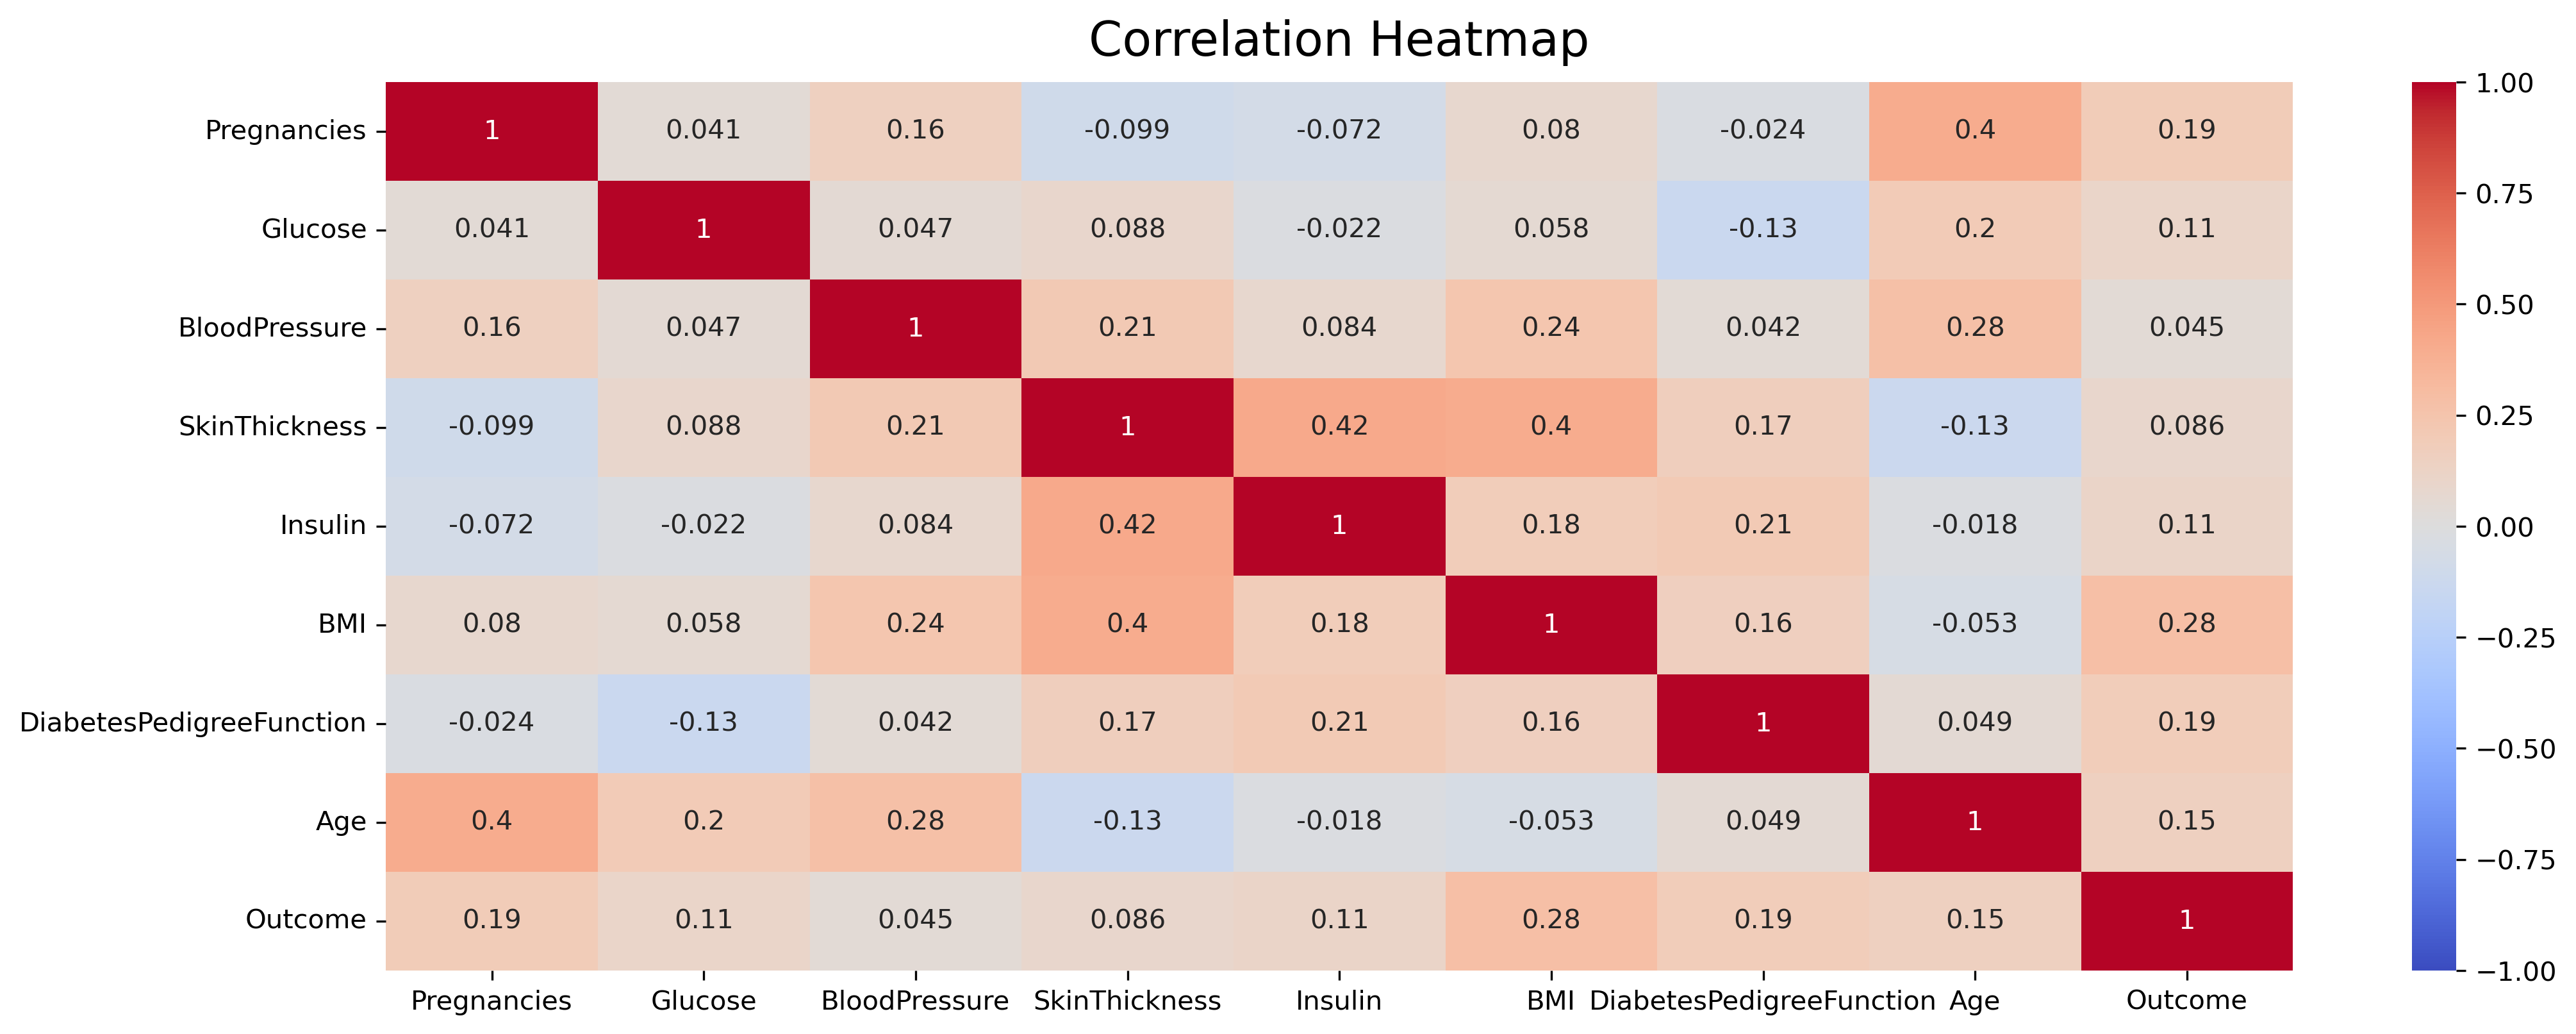
\includegraphics[width=1\linewidth]{../HW2_2/CorrelationHeatmap.png}}
		\caption{نمودار وابستگی داده‌ها}
		\label{fig:correlation2}
	\end{figure}\\
	برای اصلاح داده‌ها ابتدا با رسم چندین نمودار با توزیع داده‌ها آشنا می‌شویم. 
	\autoref{fig:hist1}
	تعداد تکرار داده‌های خام را نشان می‌دهند.
	\begin{figure*}[!h]
		\centering
		\subfigure[]{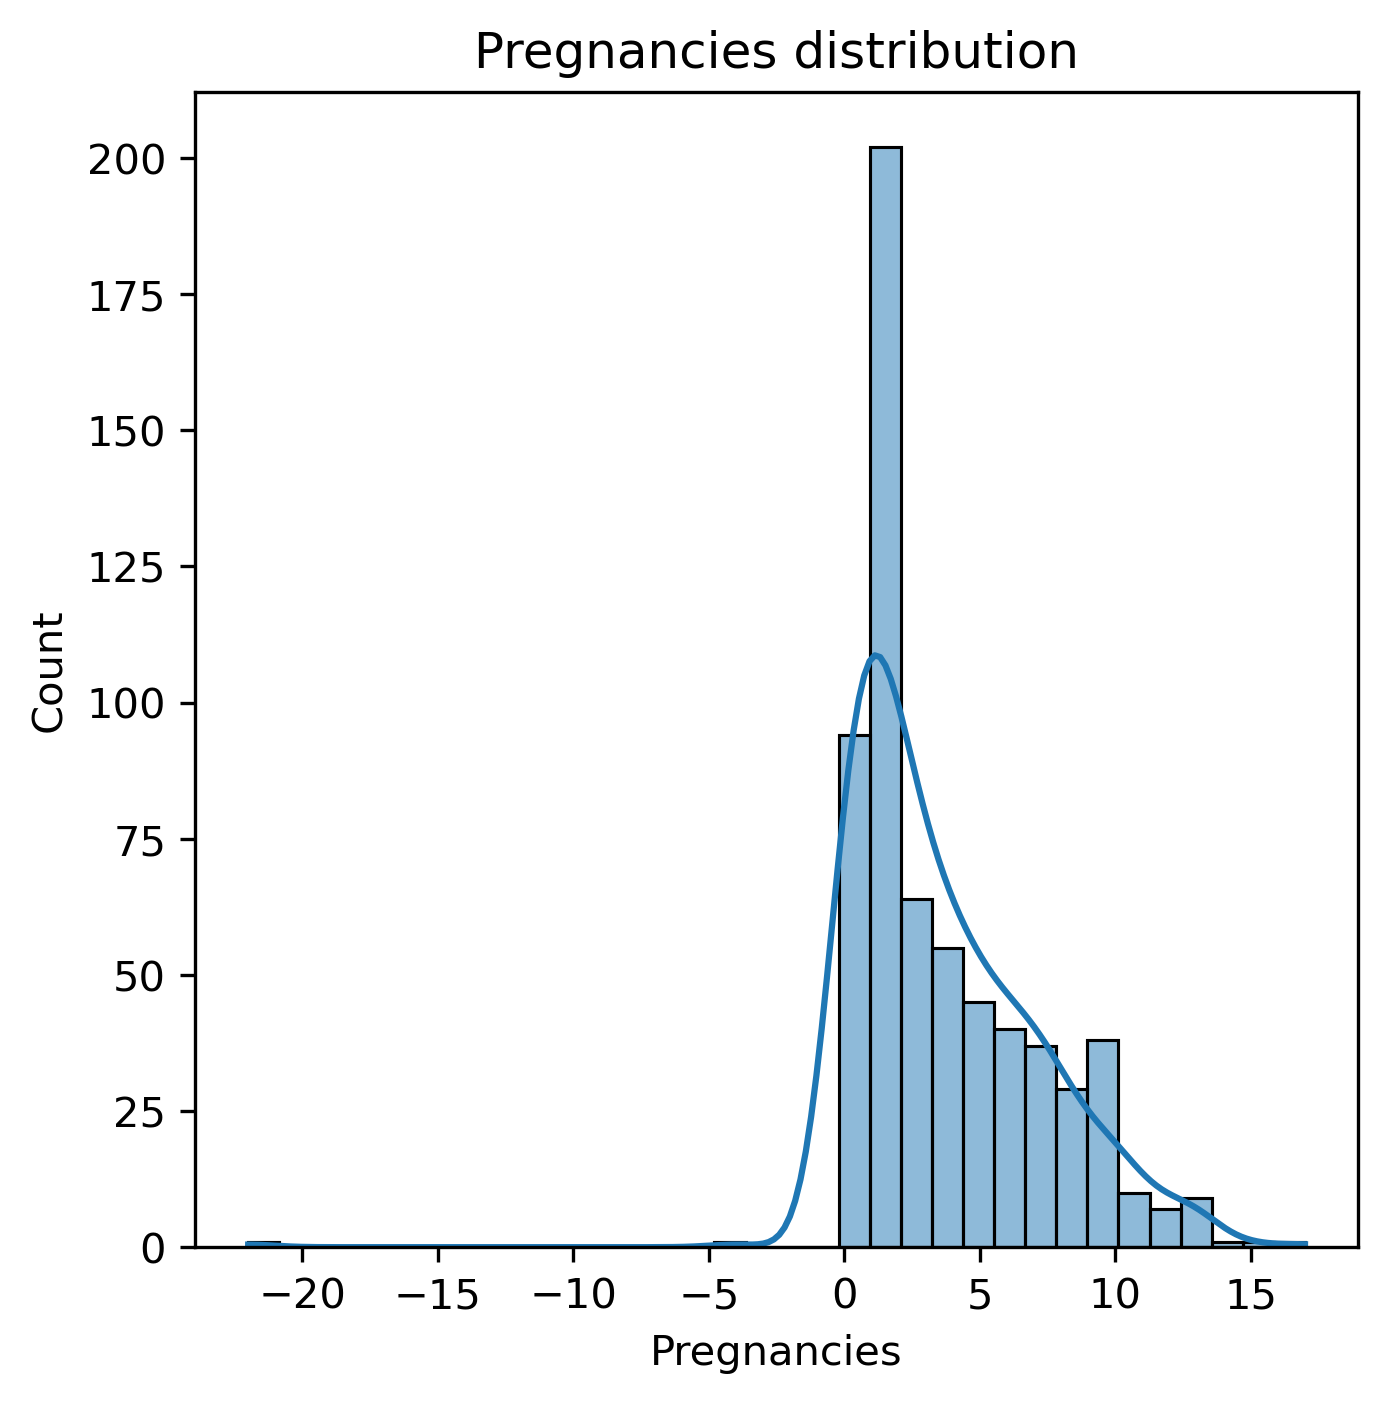
\includegraphics[height=0.31\linewidth]{../HW2_2/Pregnancies distribution.png}}
		\subfigure[]{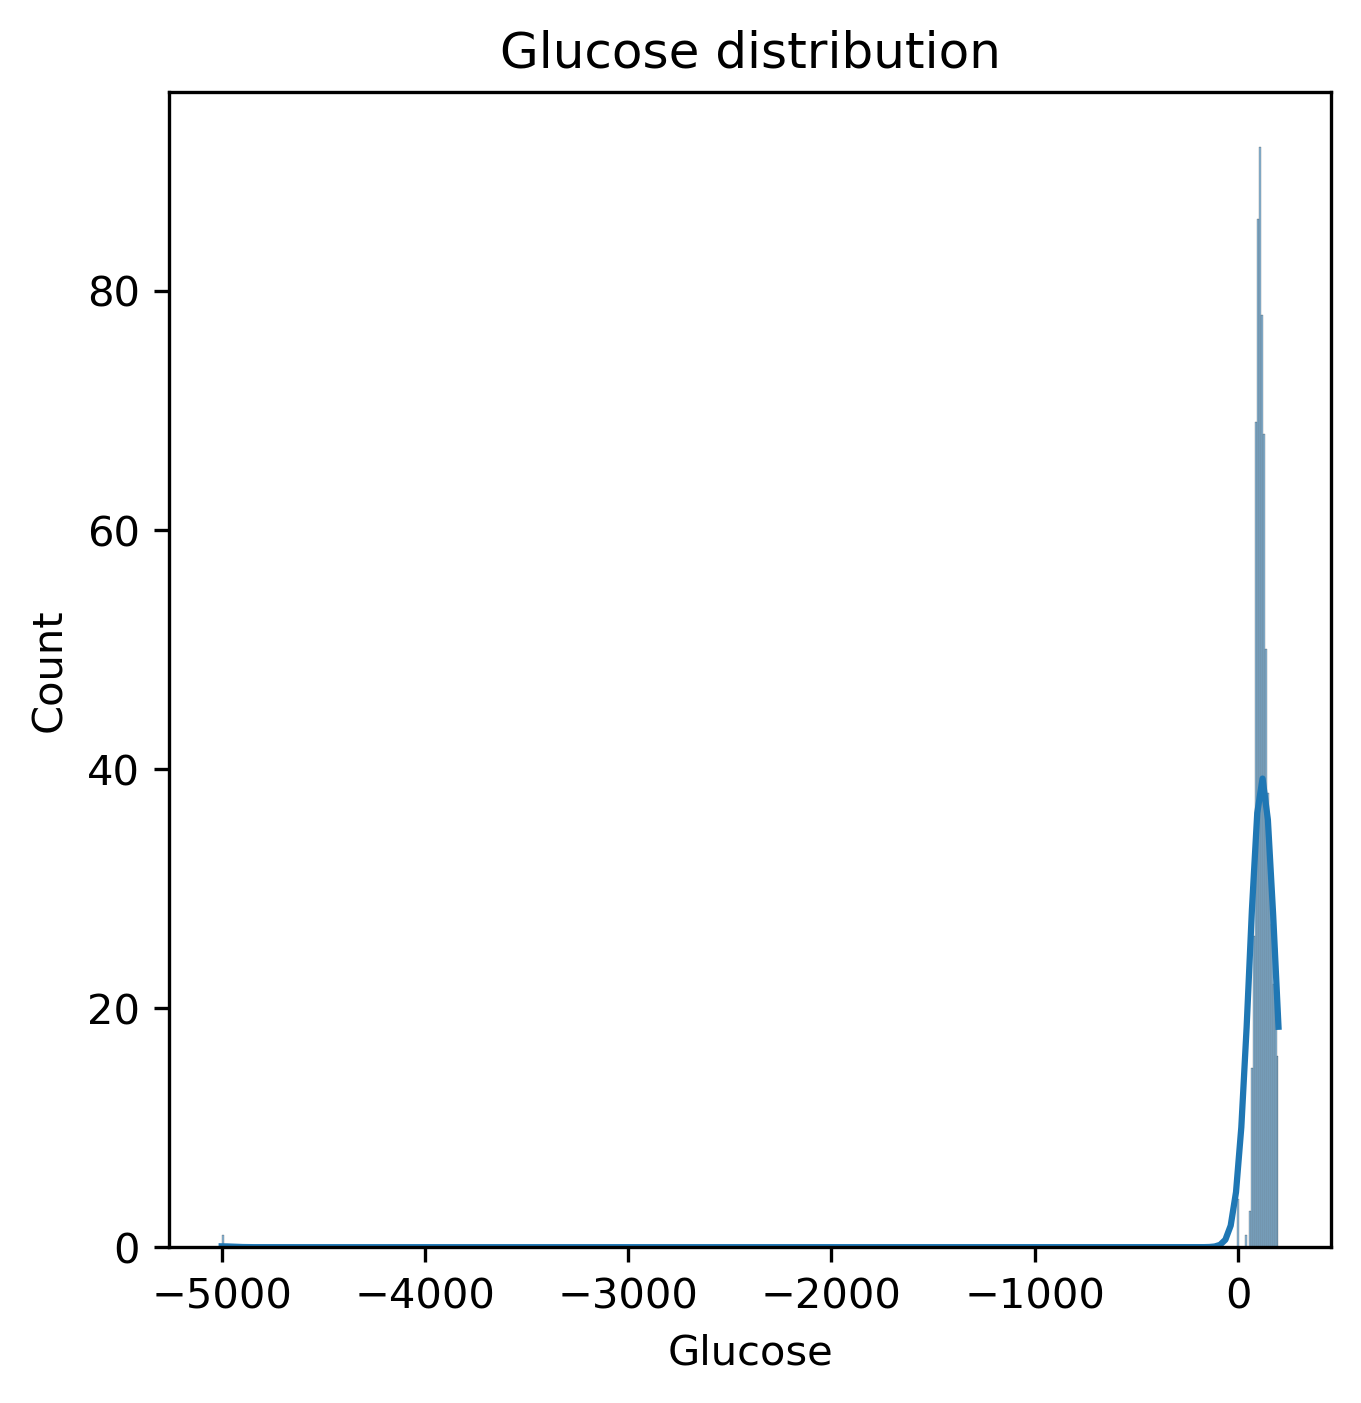
\includegraphics[height=0.31\linewidth]{../HW2_2/Glucose distribution.png}}
		\subfigure[]{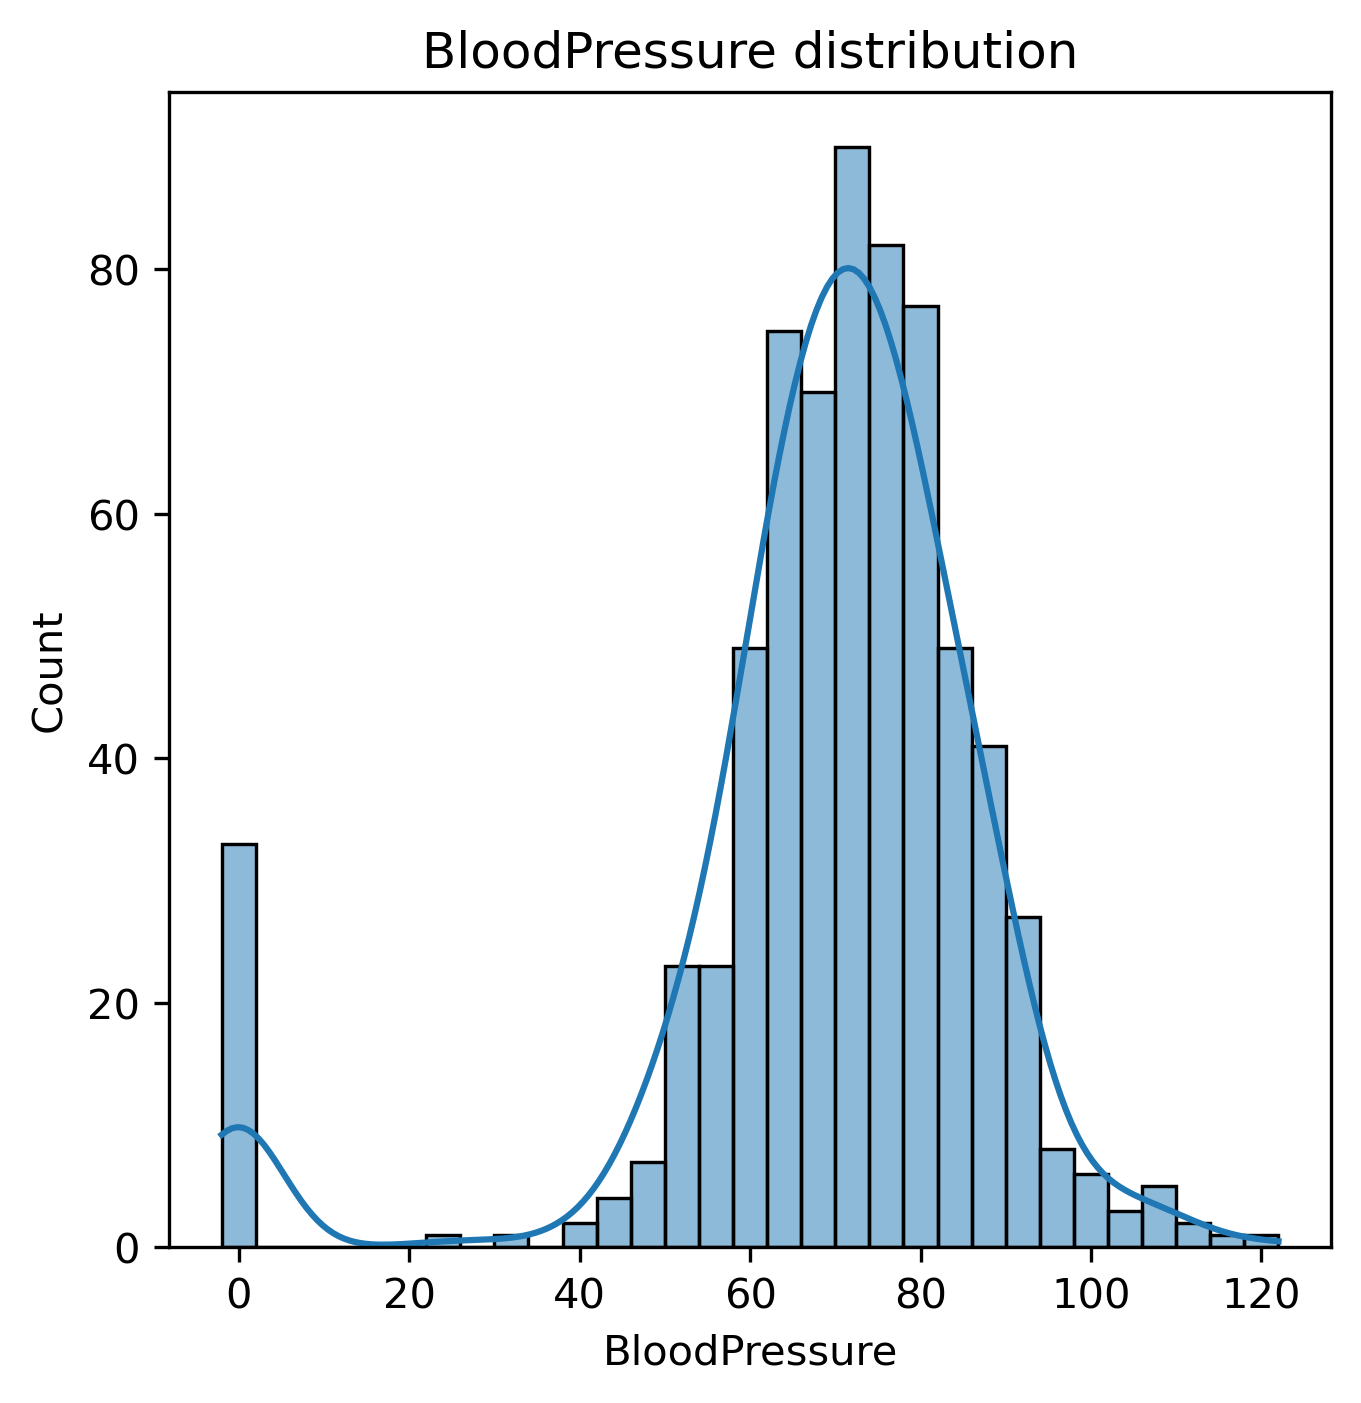
\includegraphics[height=0.31\linewidth]{../HW2_2/BloodPressure distribution.png}}
		\subfigure[]{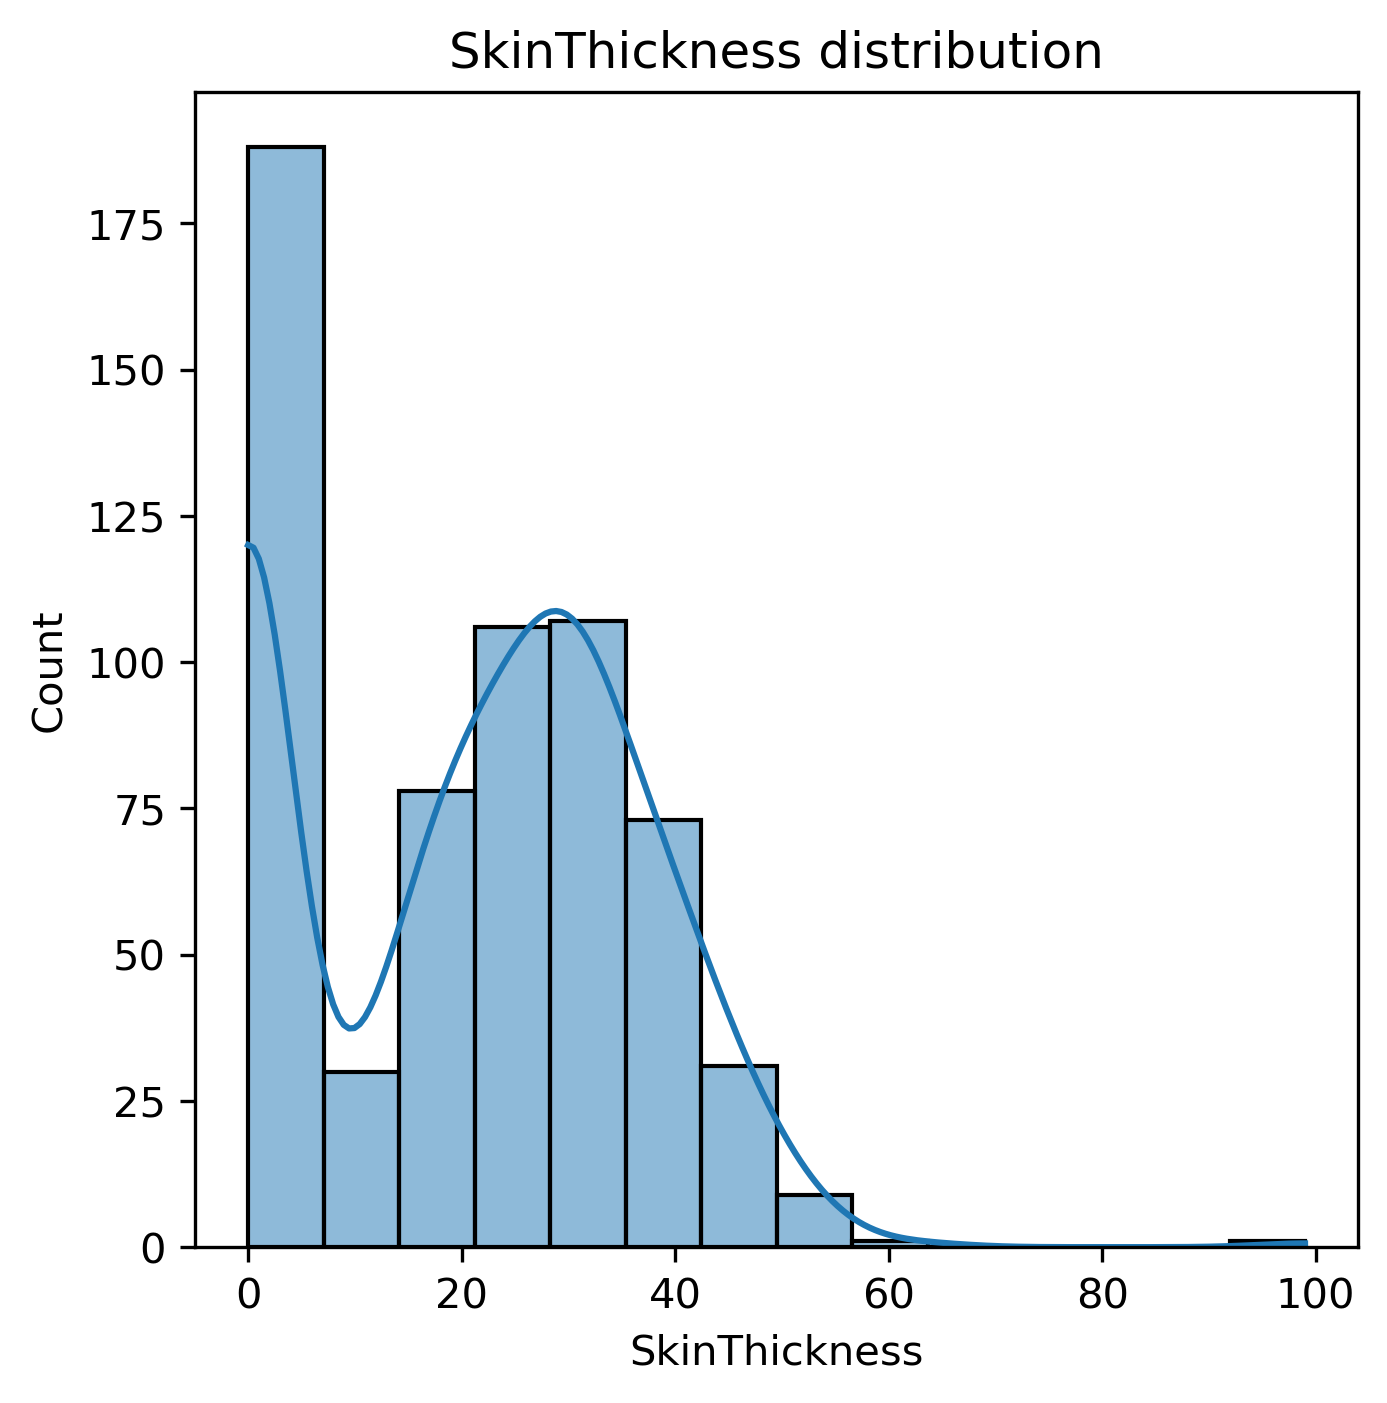
\includegraphics[height=0.31\linewidth]{../HW2_2/SkinThickness distribution.png}}
		\subfigure[]{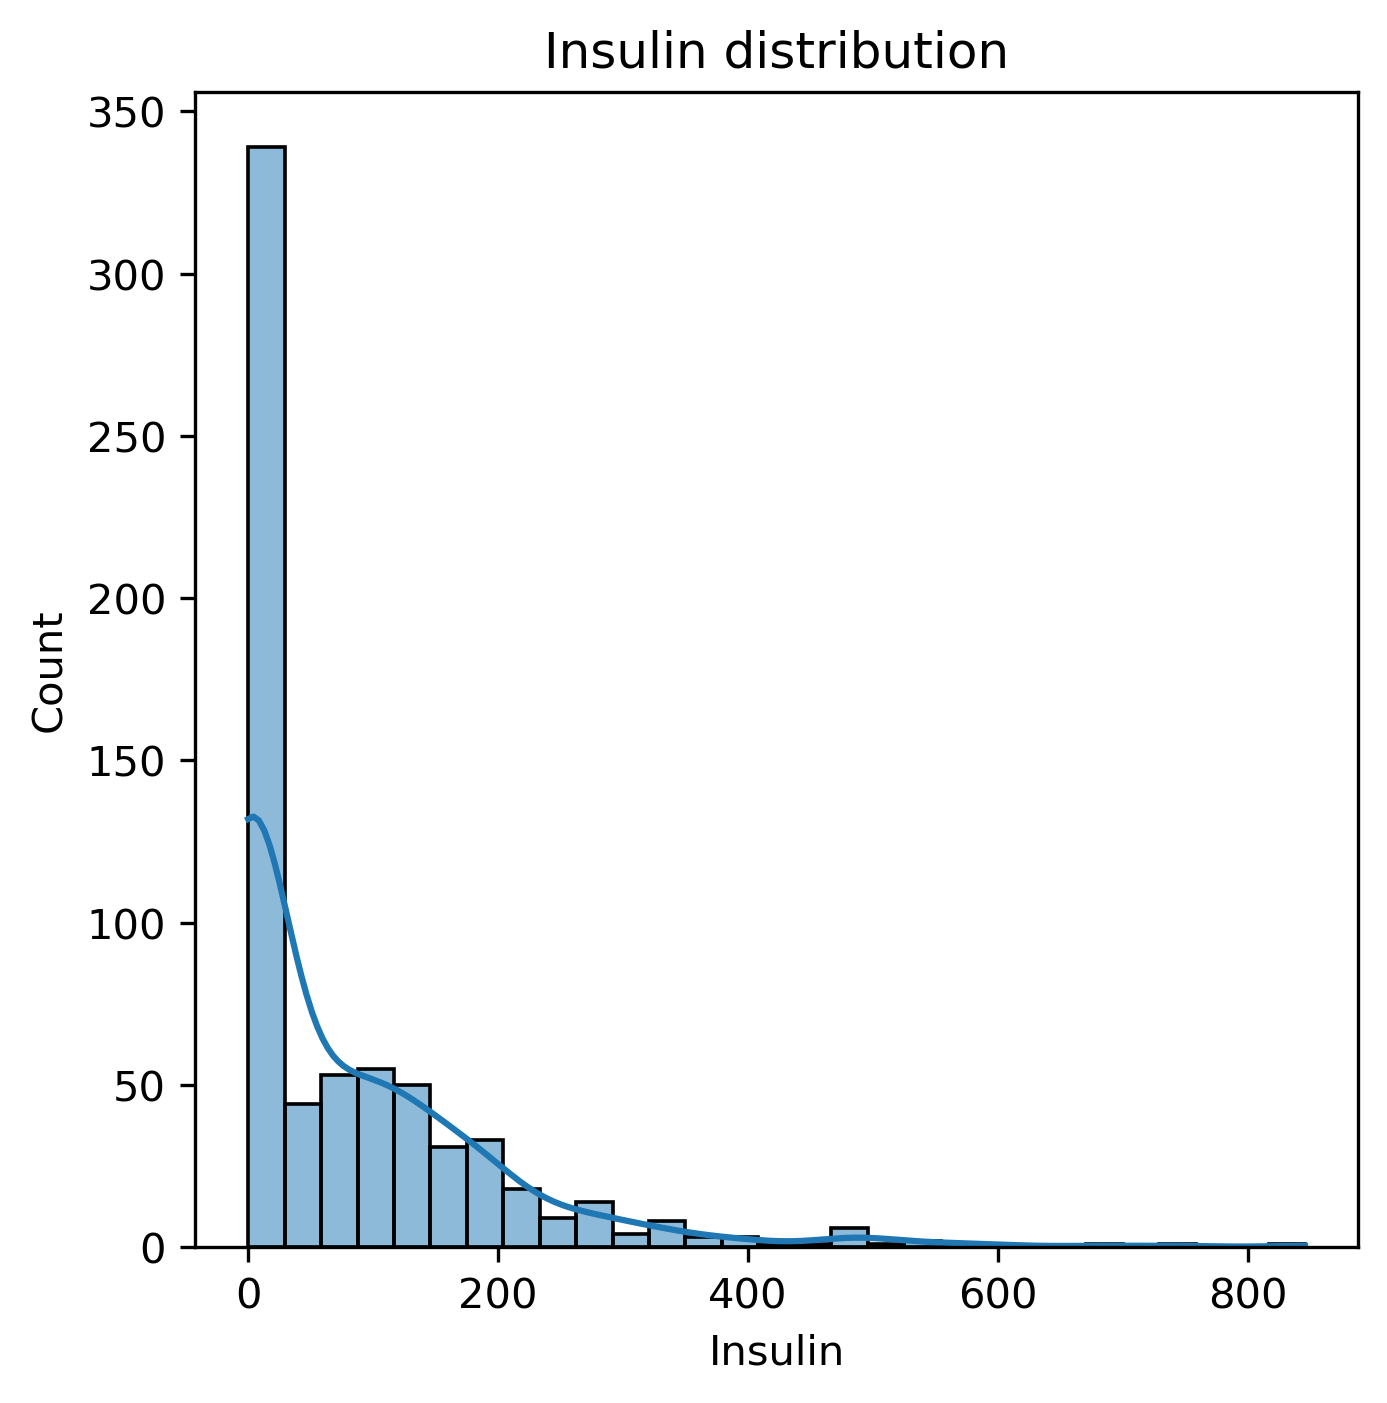
\includegraphics[height=0.31\linewidth]{../HW2_2/Insulin distribution.png}}
		\subfigure[]{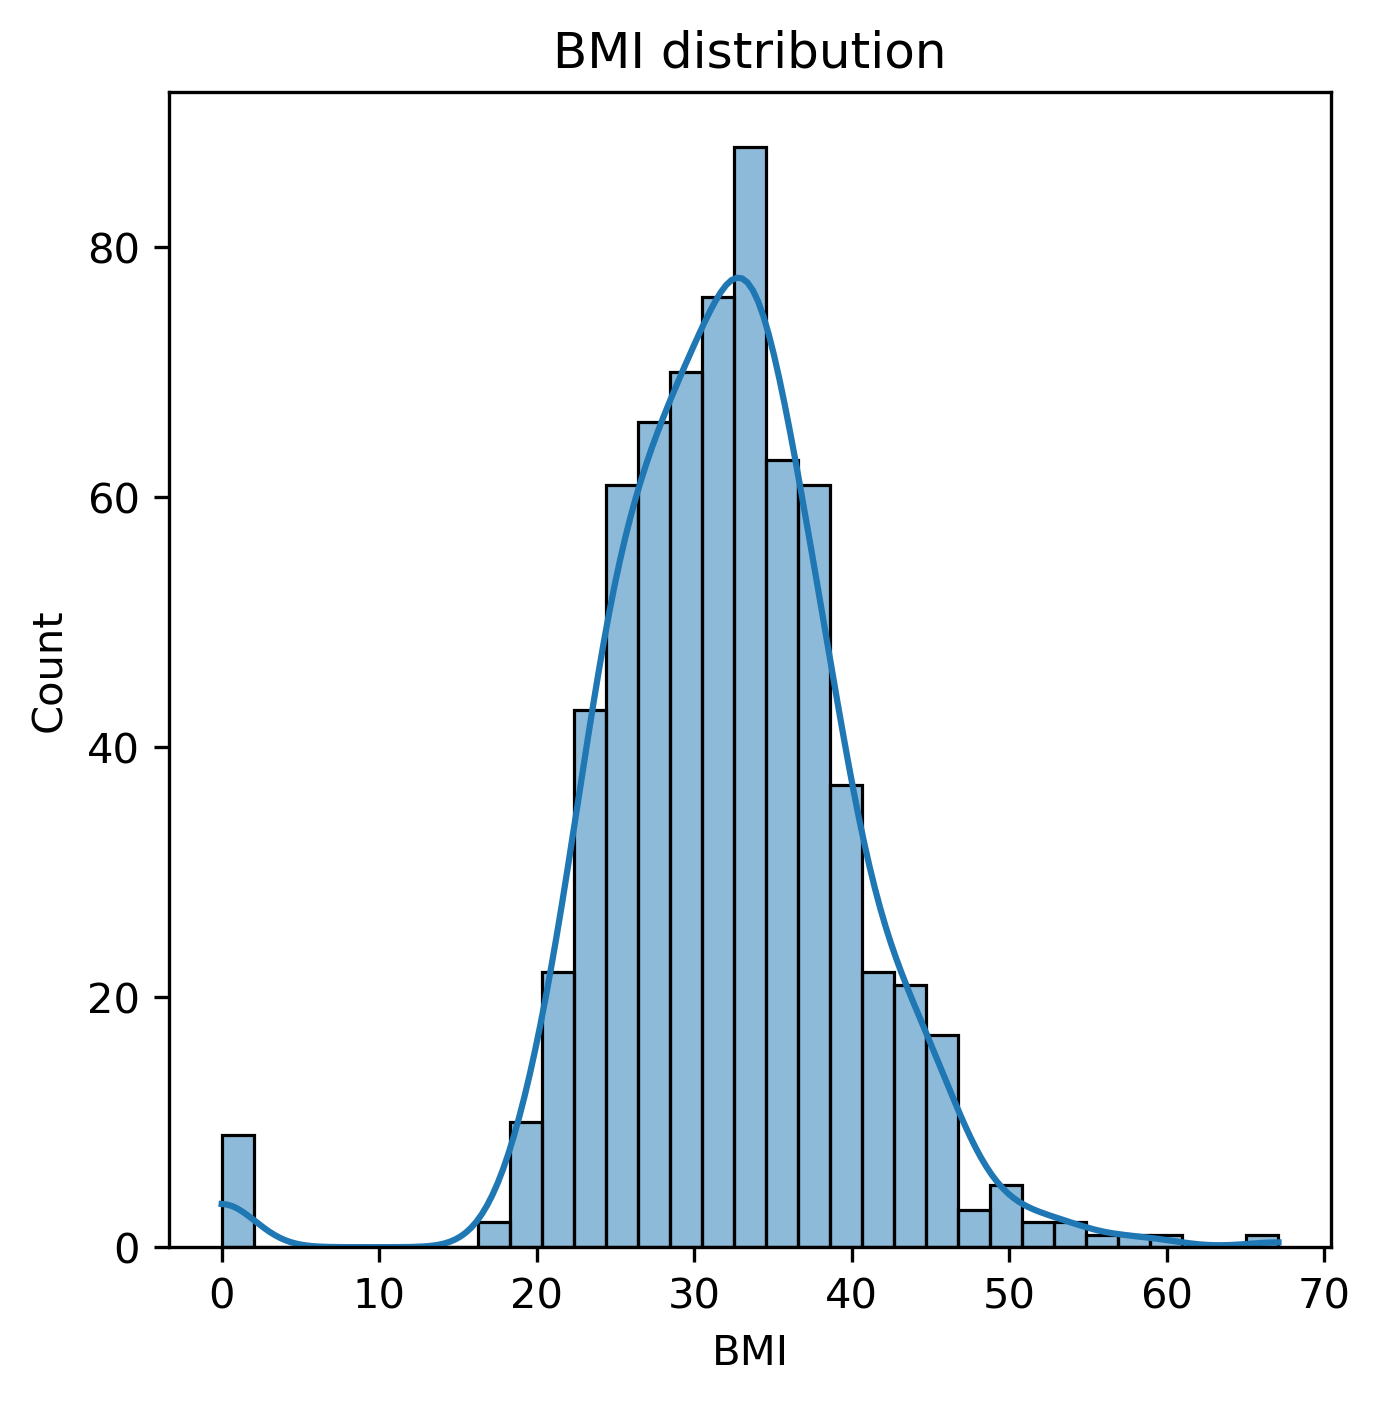
\includegraphics[height=0.31\linewidth]{../HW2_2/BMI distribution.png}}
		\subfigure[]{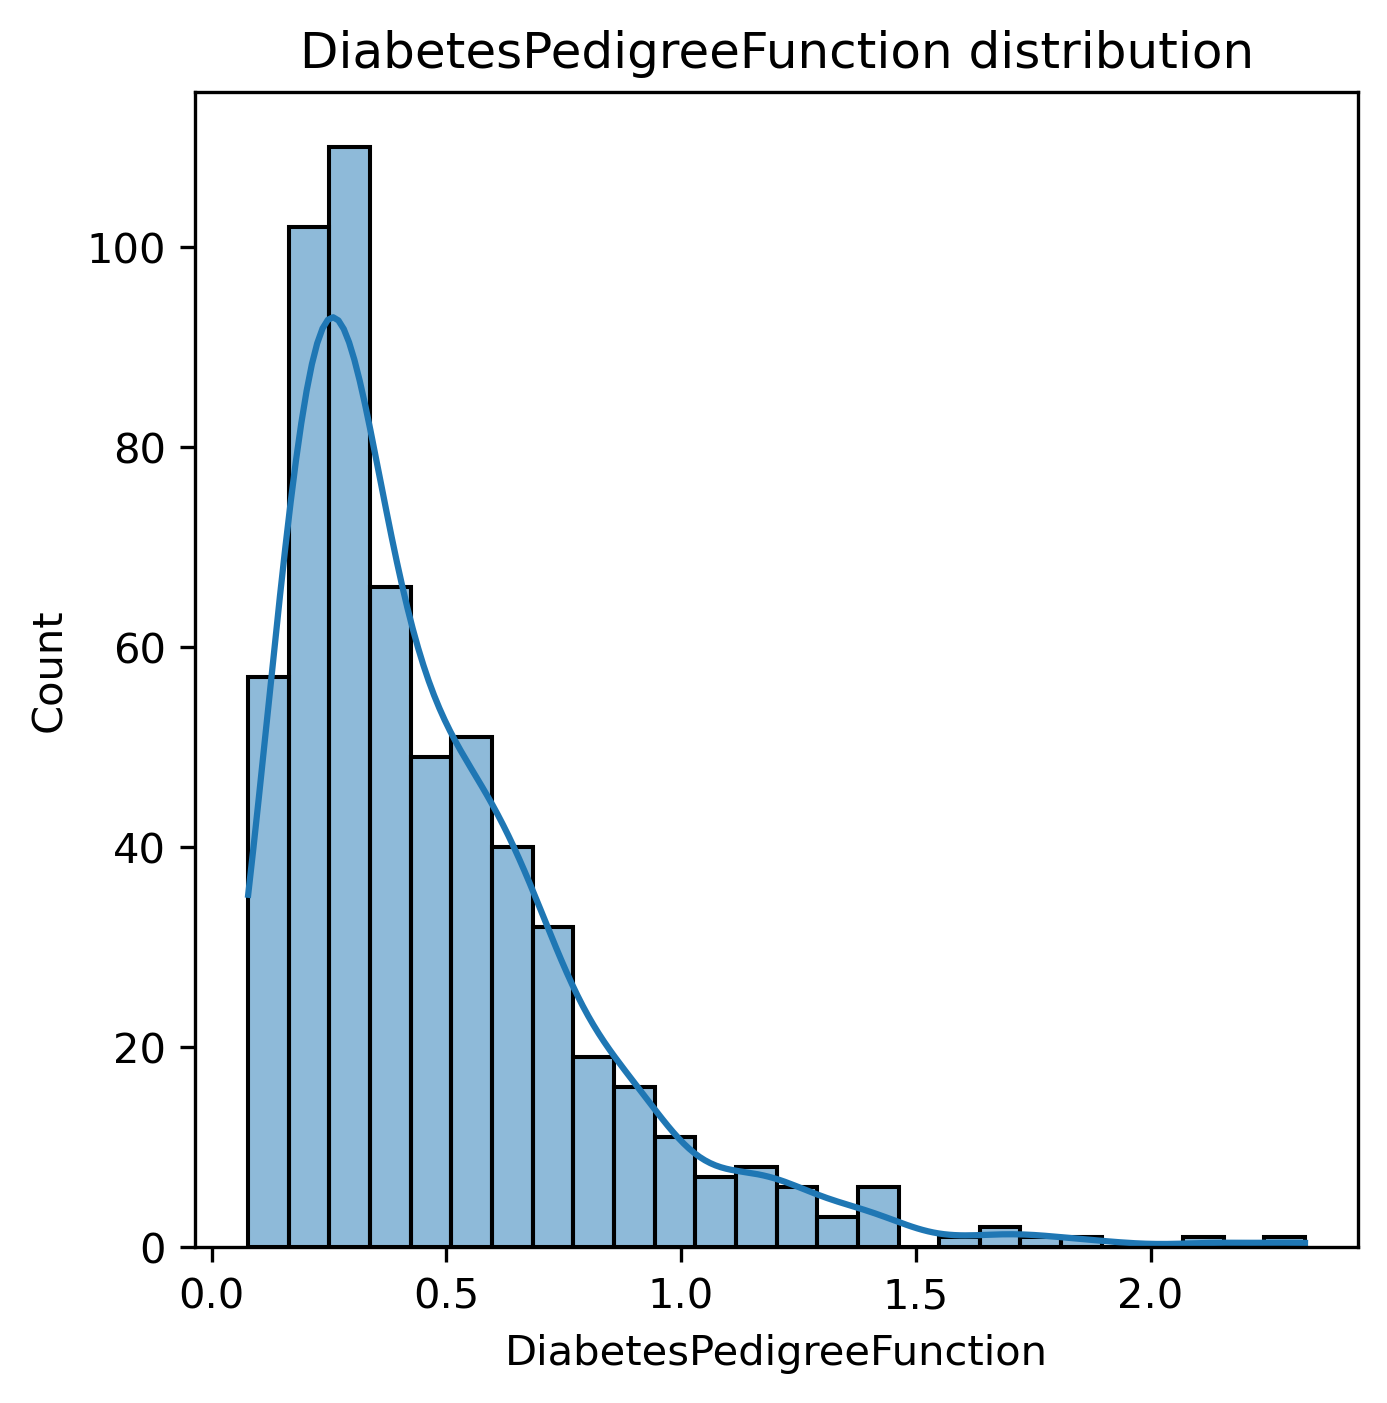
\includegraphics[height=0.31\linewidth]{../HW2_2/DiabetesPedigreeFunction distribution.png}}
		\subfigure[]{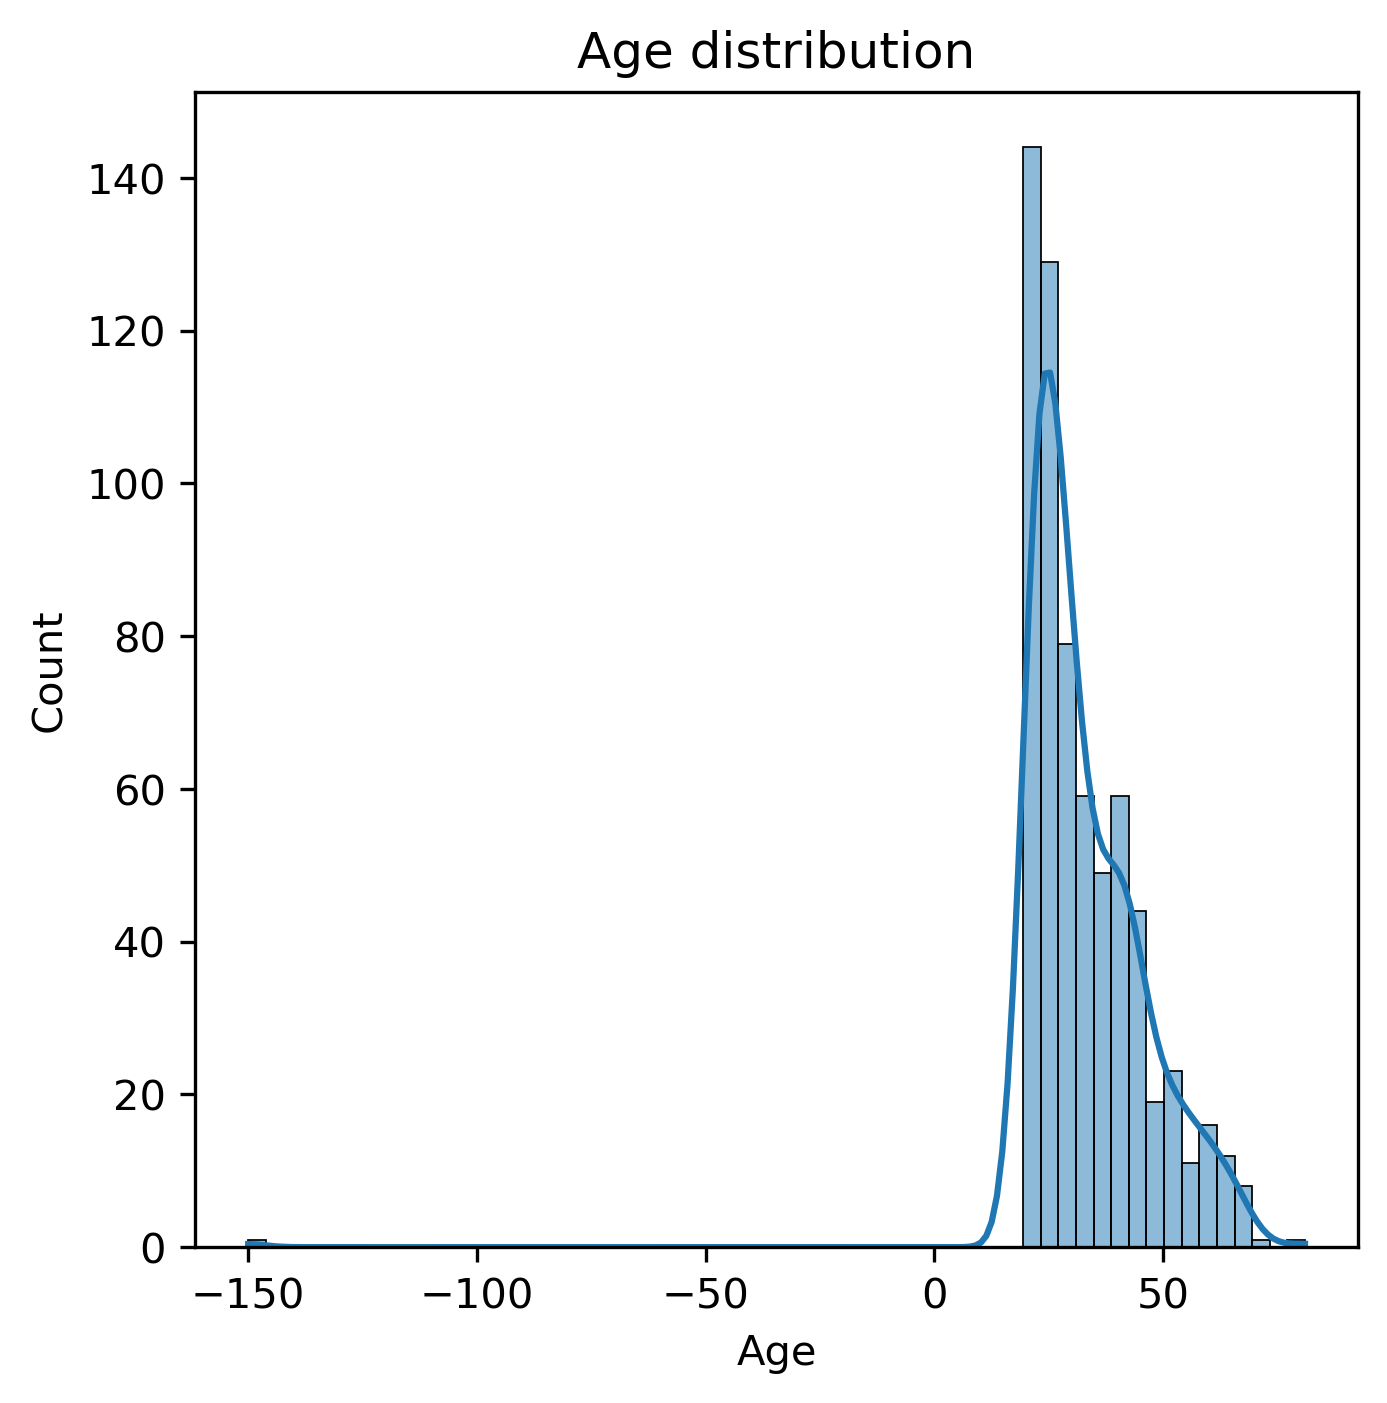
\includegraphics[height=0.31\linewidth]{../HW2_2/Age distribution.png}}
		\caption{توزیع داده‌های خام به صورت هیستوگرام}
		\label{fig:hist1}
	\end{figure*}
	
	
	نمودار‌های 
	\lr{scatter}
	در
	\autoref{fig:scatter}
	و نمودار‌های 
	\lr{hexbin}
	در
	\autoref{fig:hexbin}
	قابل مشاهده هستند.
	\begin{figure*}[!h]
		\centering
		\subfigure[]{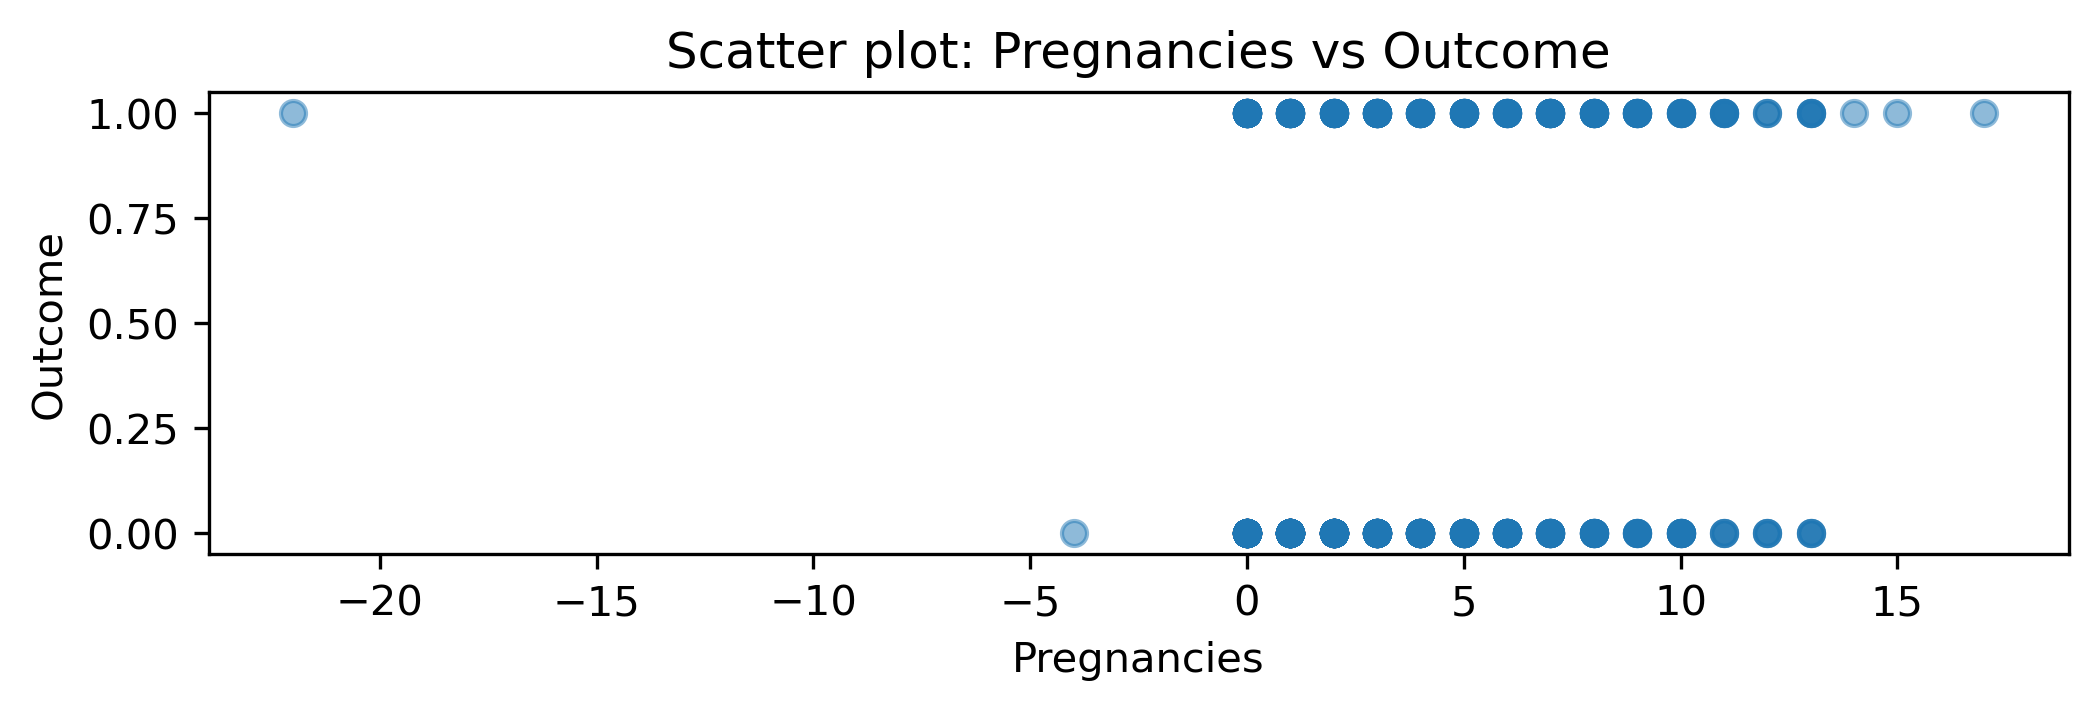
\includegraphics[height=0.15\linewidth]{../HW2_2/Pregnancies scatter.png}}
		\subfigure[]{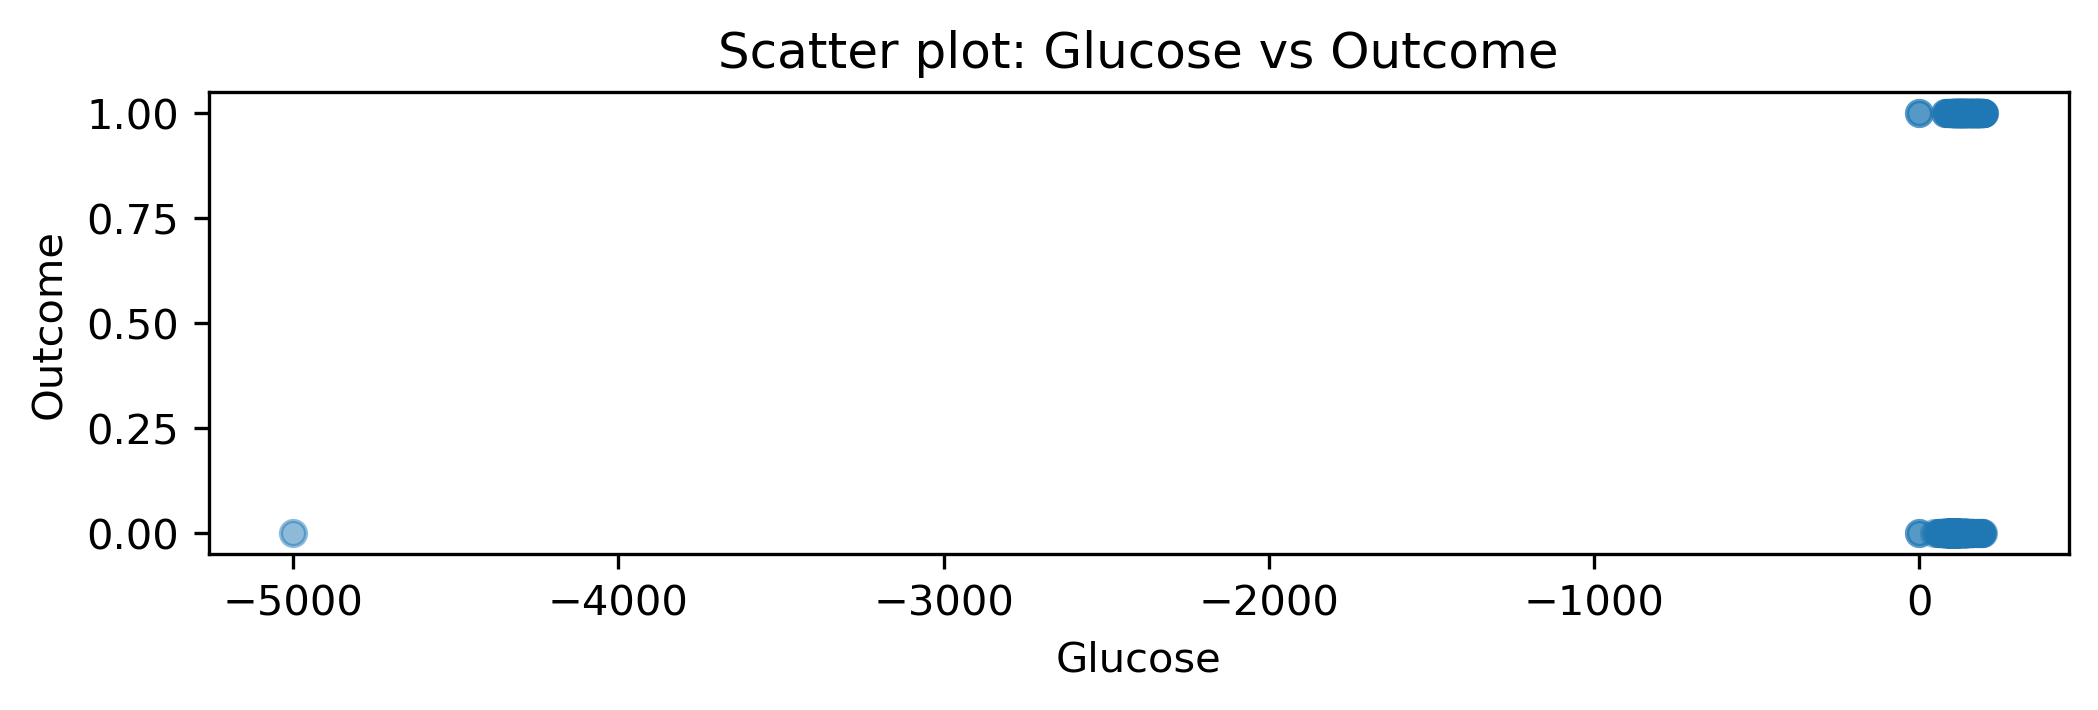
\includegraphics[height=0.15\linewidth]{../HW2_2/Glucose scatter.png}}
		\subfigure[]{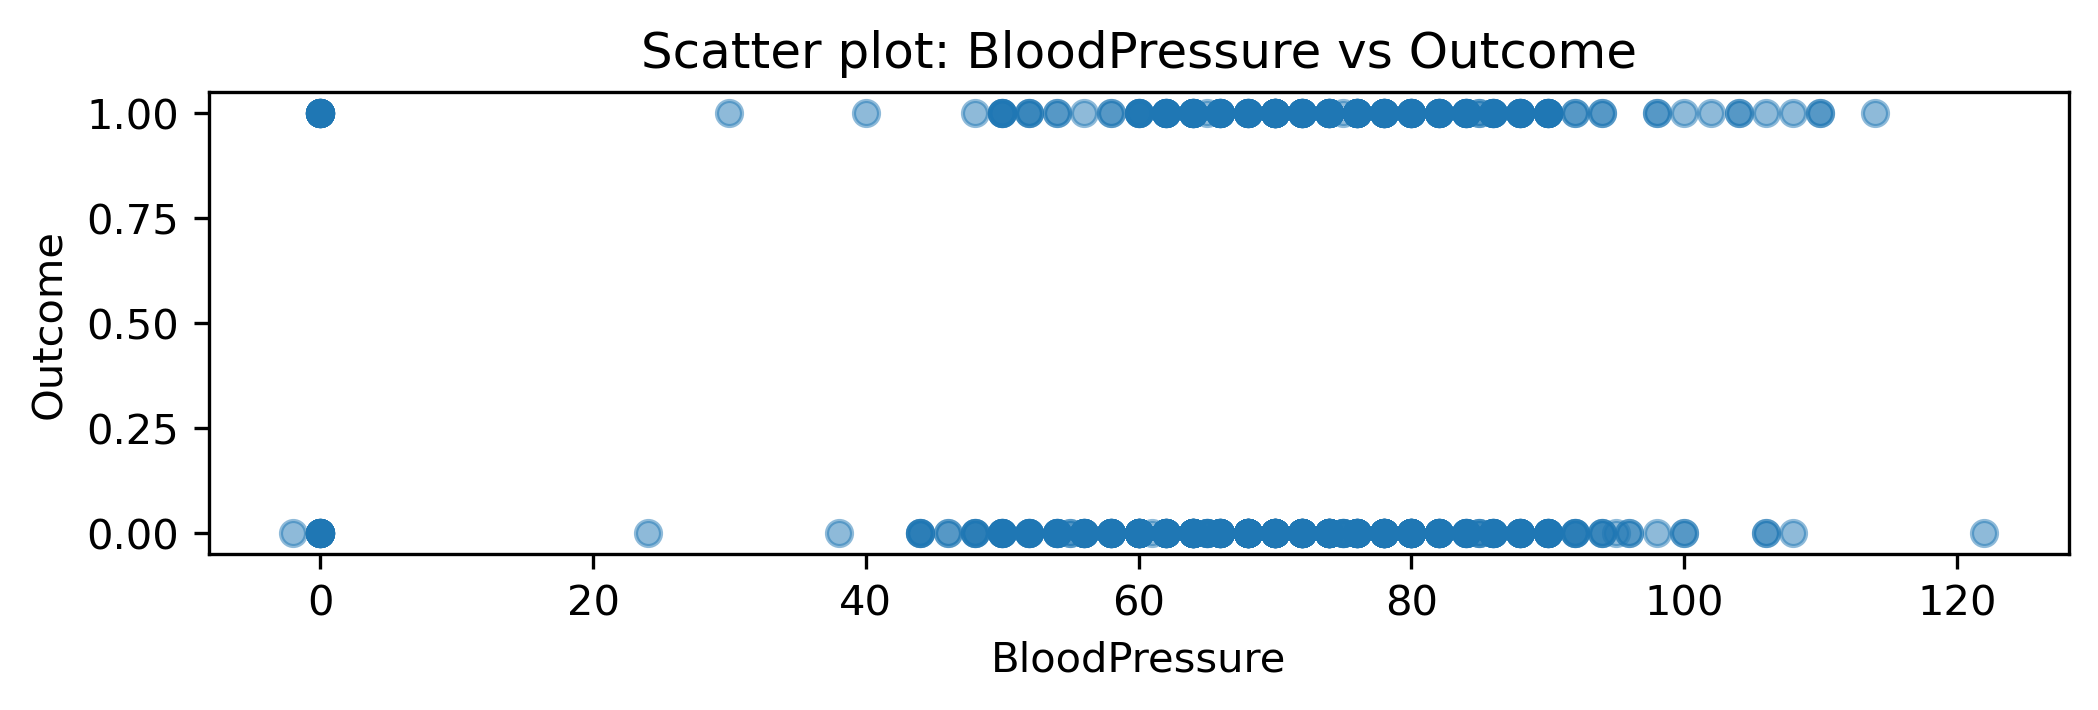
\includegraphics[height=0.15\linewidth]{../HW2_2/BloodPressure scatter.png}}
		\subfigure[]{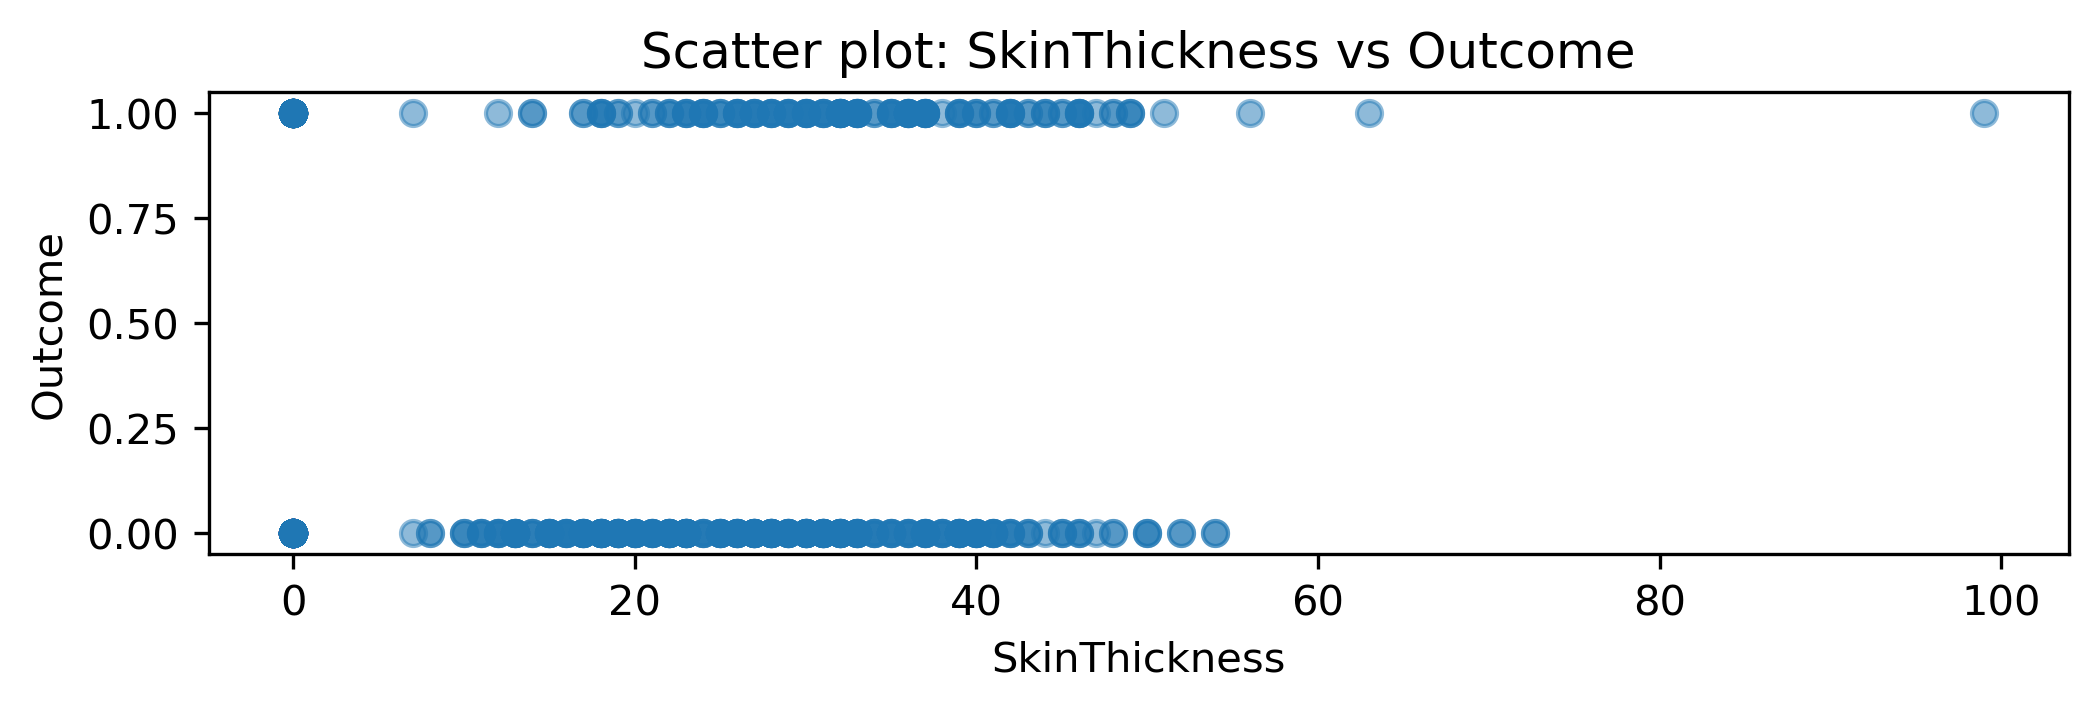
\includegraphics[height=0.15\linewidth]{../HW2_2/SkinThickness scatter.png}}
		\subfigure[]{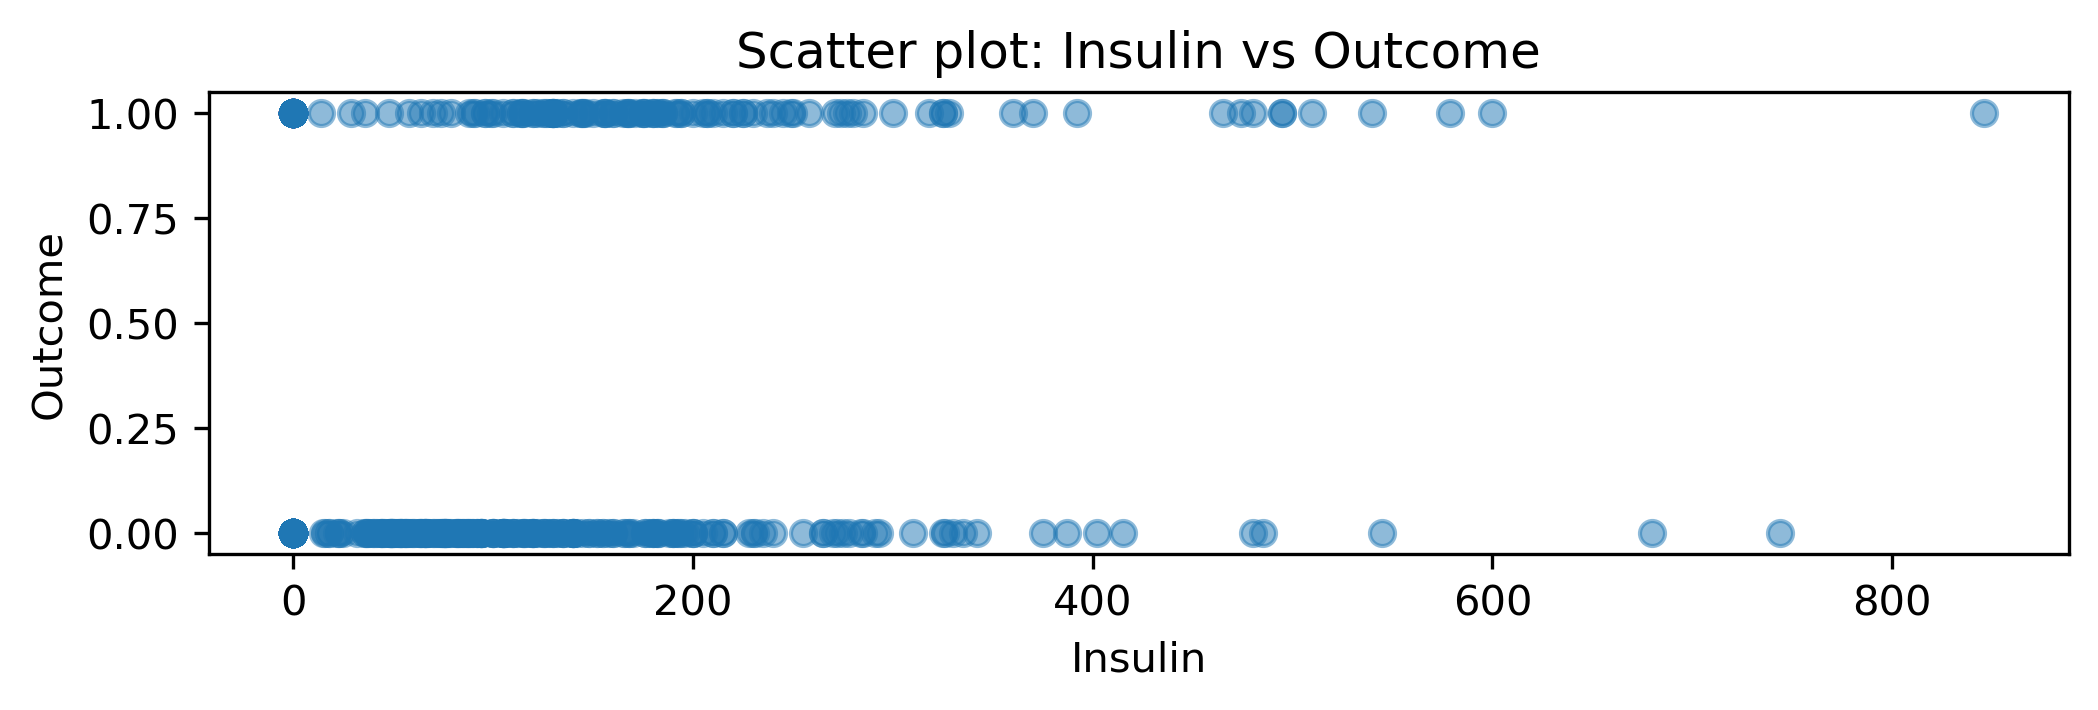
\includegraphics[height=0.15\linewidth]{../HW2_2/Insulin scatter.png}}
		\subfigure[]{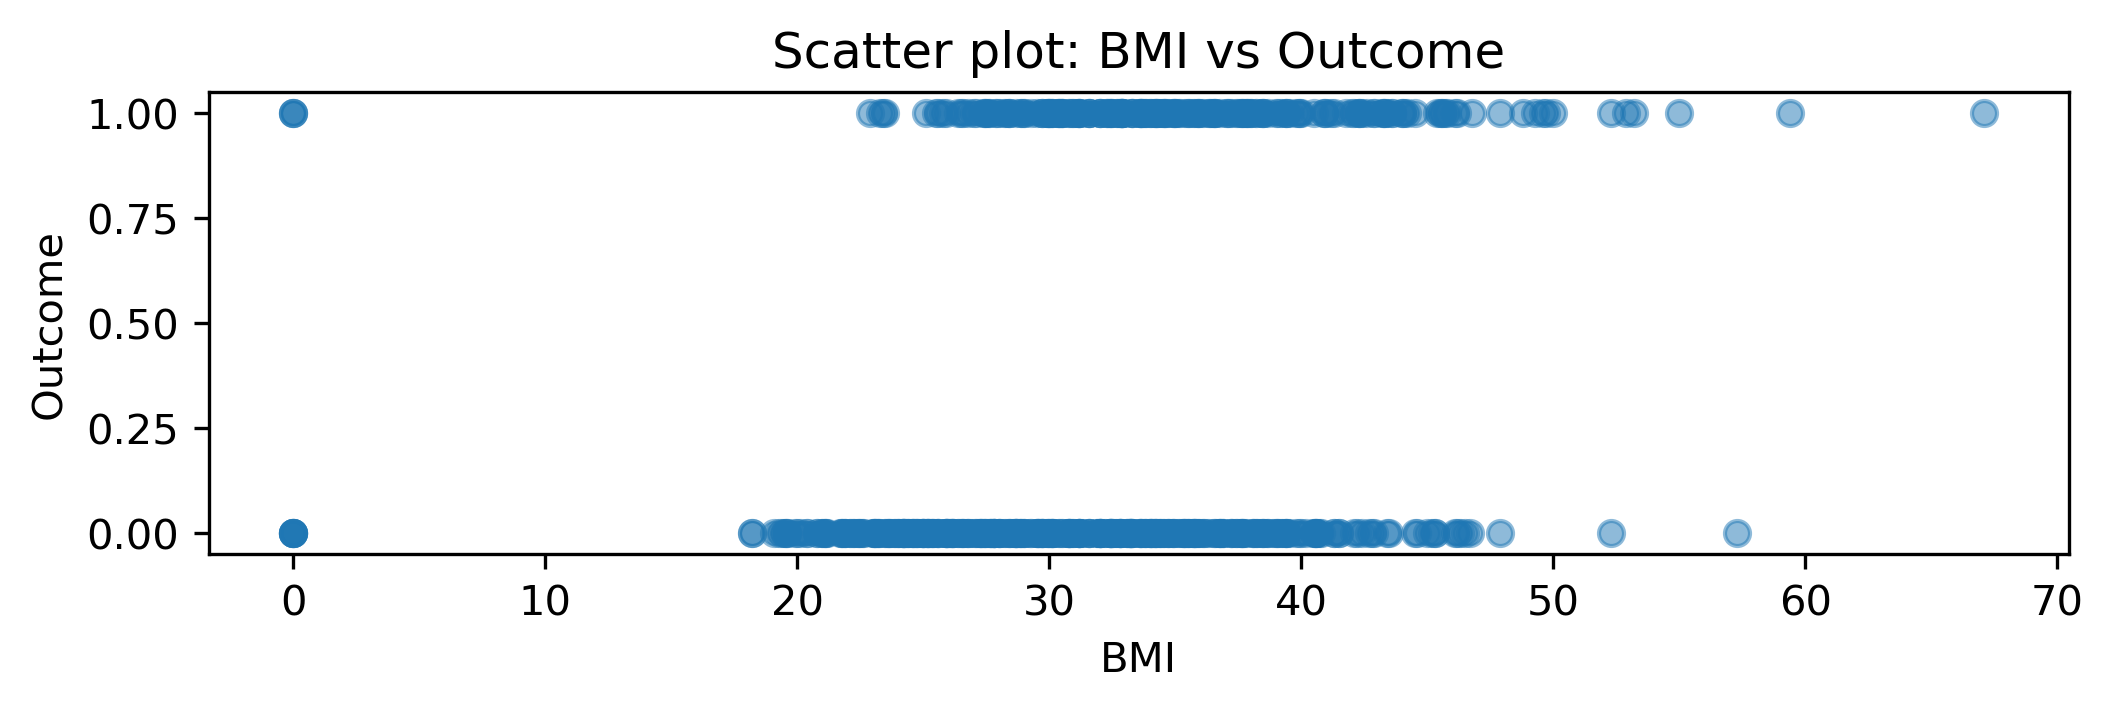
\includegraphics[height=0.15\linewidth]{../HW2_2/BMI scatter.png}}
		\subfigure[]{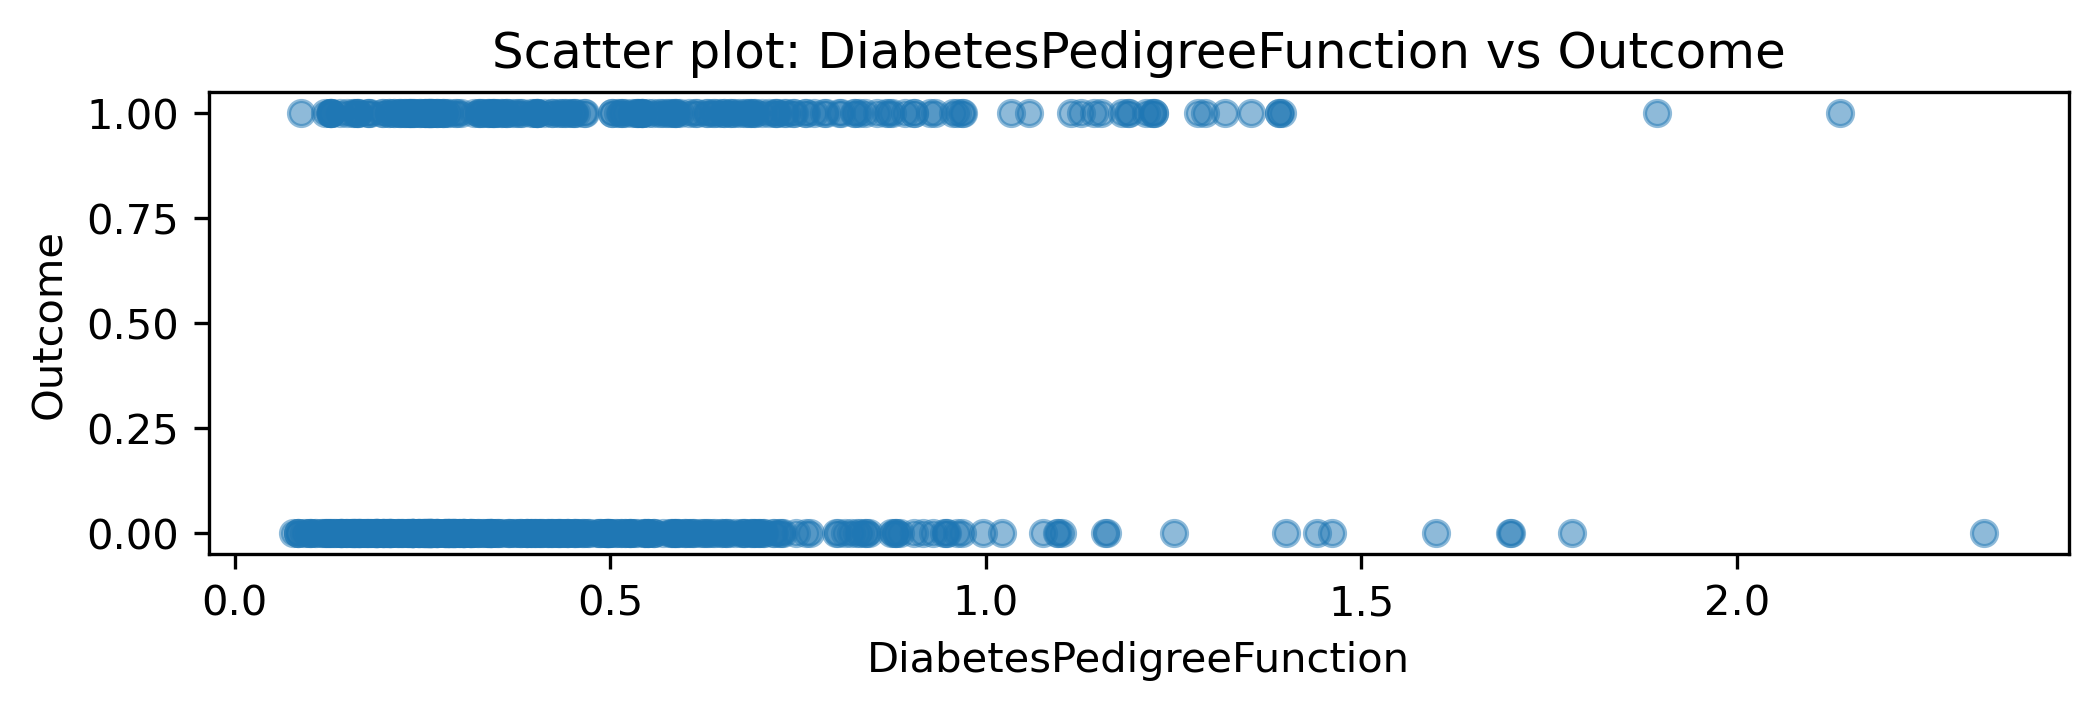
\includegraphics[height=0.15\linewidth]{../HW2_2/DiabetesPedigreeFunction scatter.png}}
		\subfigure[]{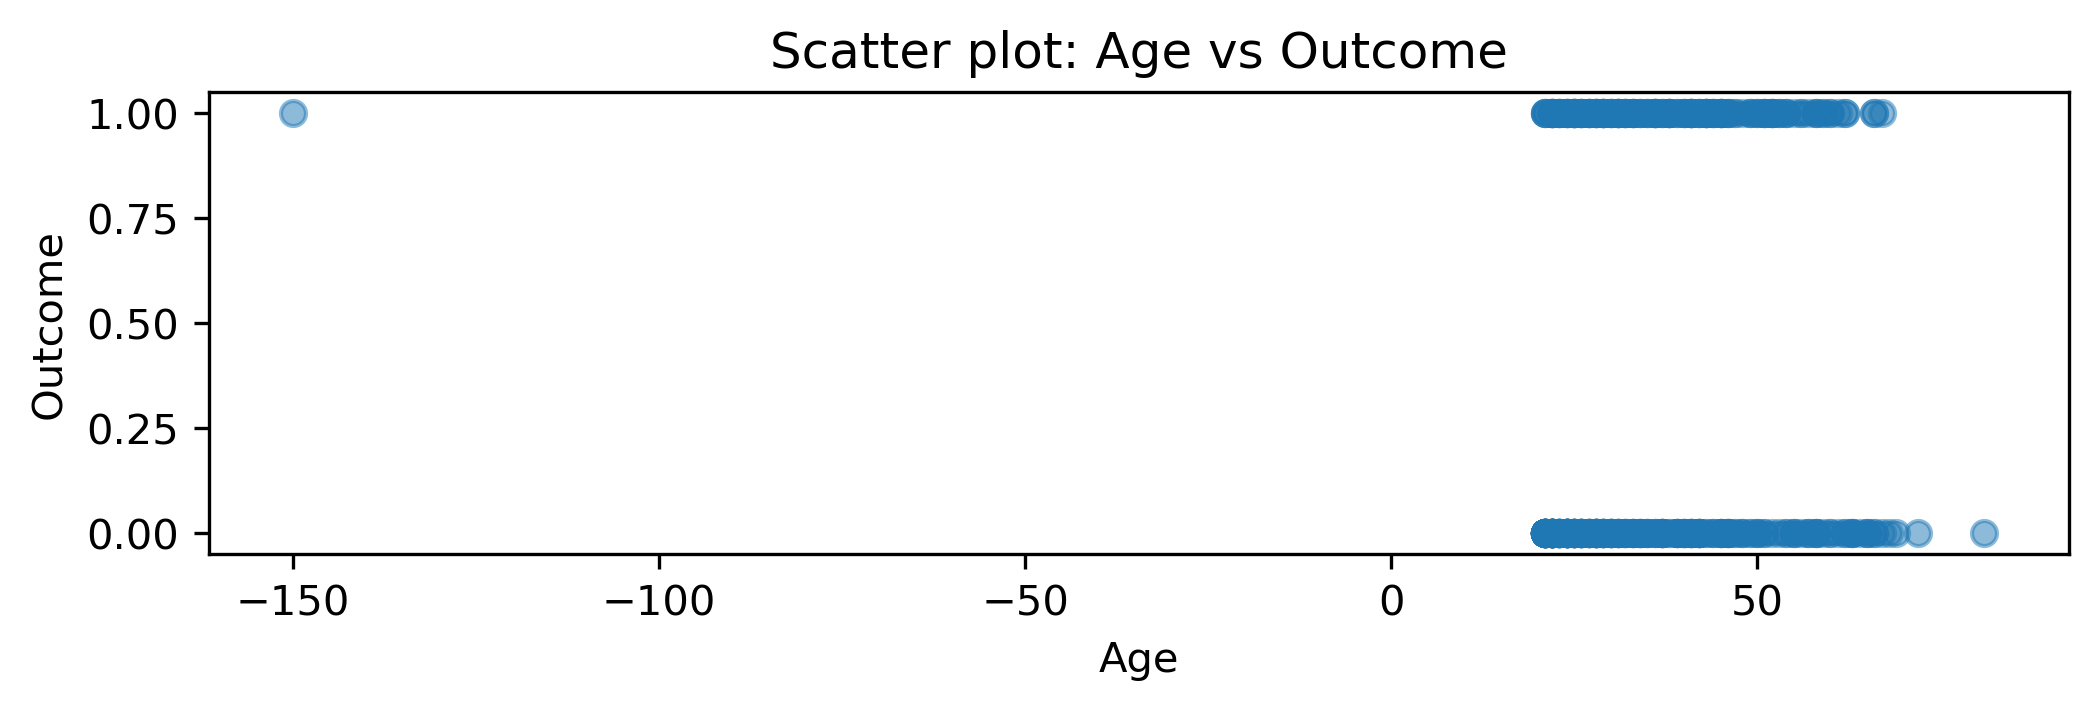
\includegraphics[height=0.15\linewidth]{../HW2_2/Age scatter.png}}
		\caption{توزیع داده‌های خام به صورت نمودار پراگندگی}
		\label{fig:scatter1}
	\end{figure*}
	\begin{figure*}[!h]
		\centering
		\subfigure[]{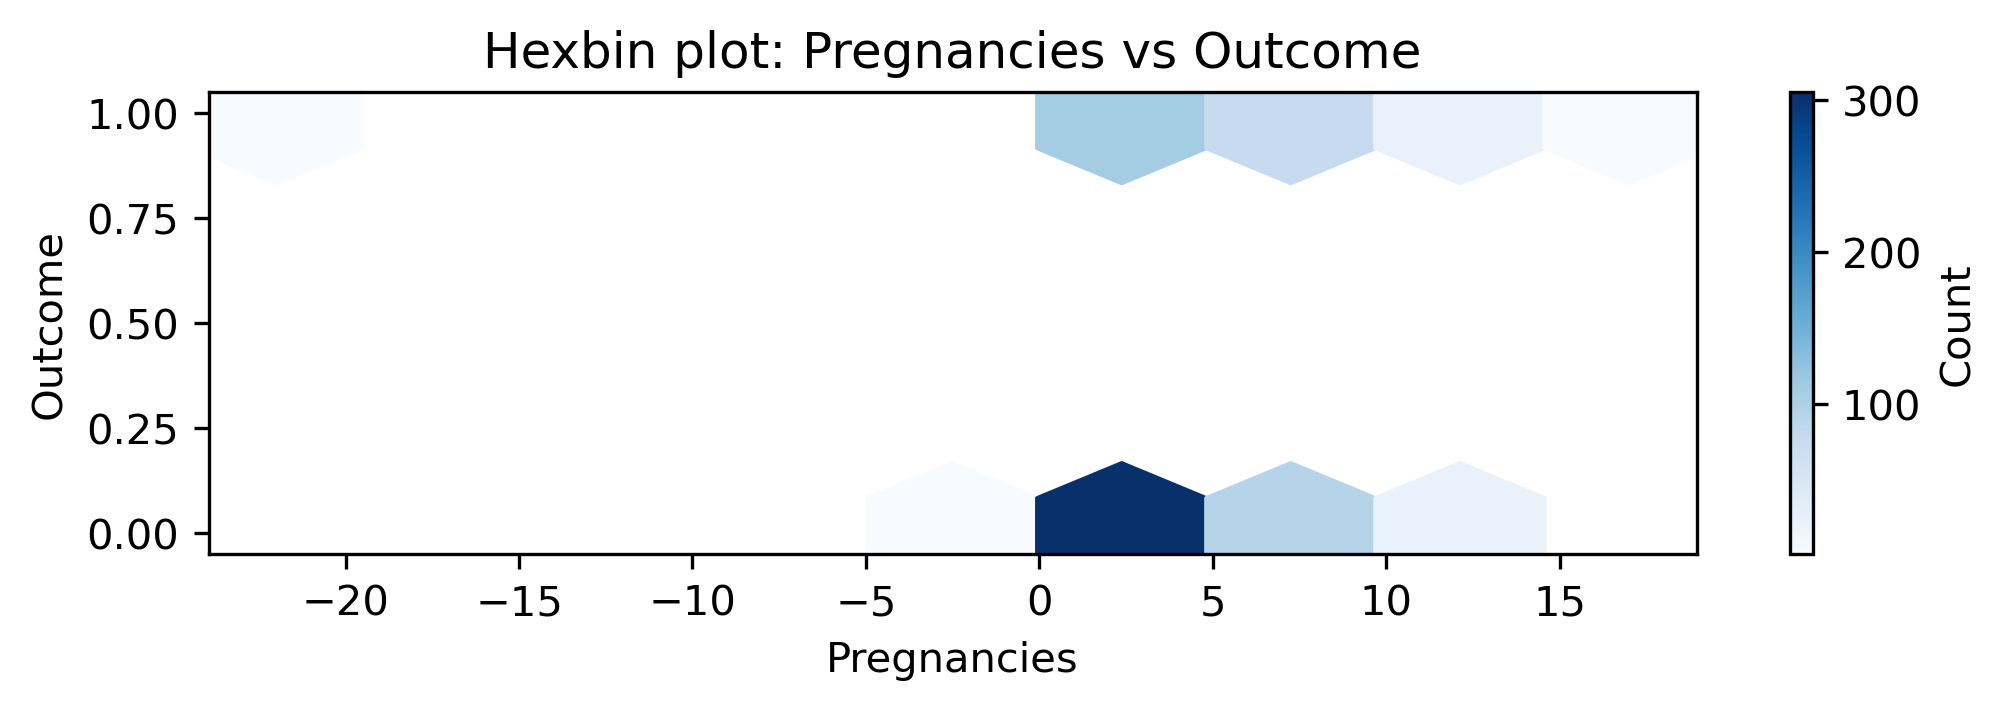
\includegraphics[height=0.15\linewidth]{../HW2_2/Pregnancies hexbin.png}}
		\subfigure[]{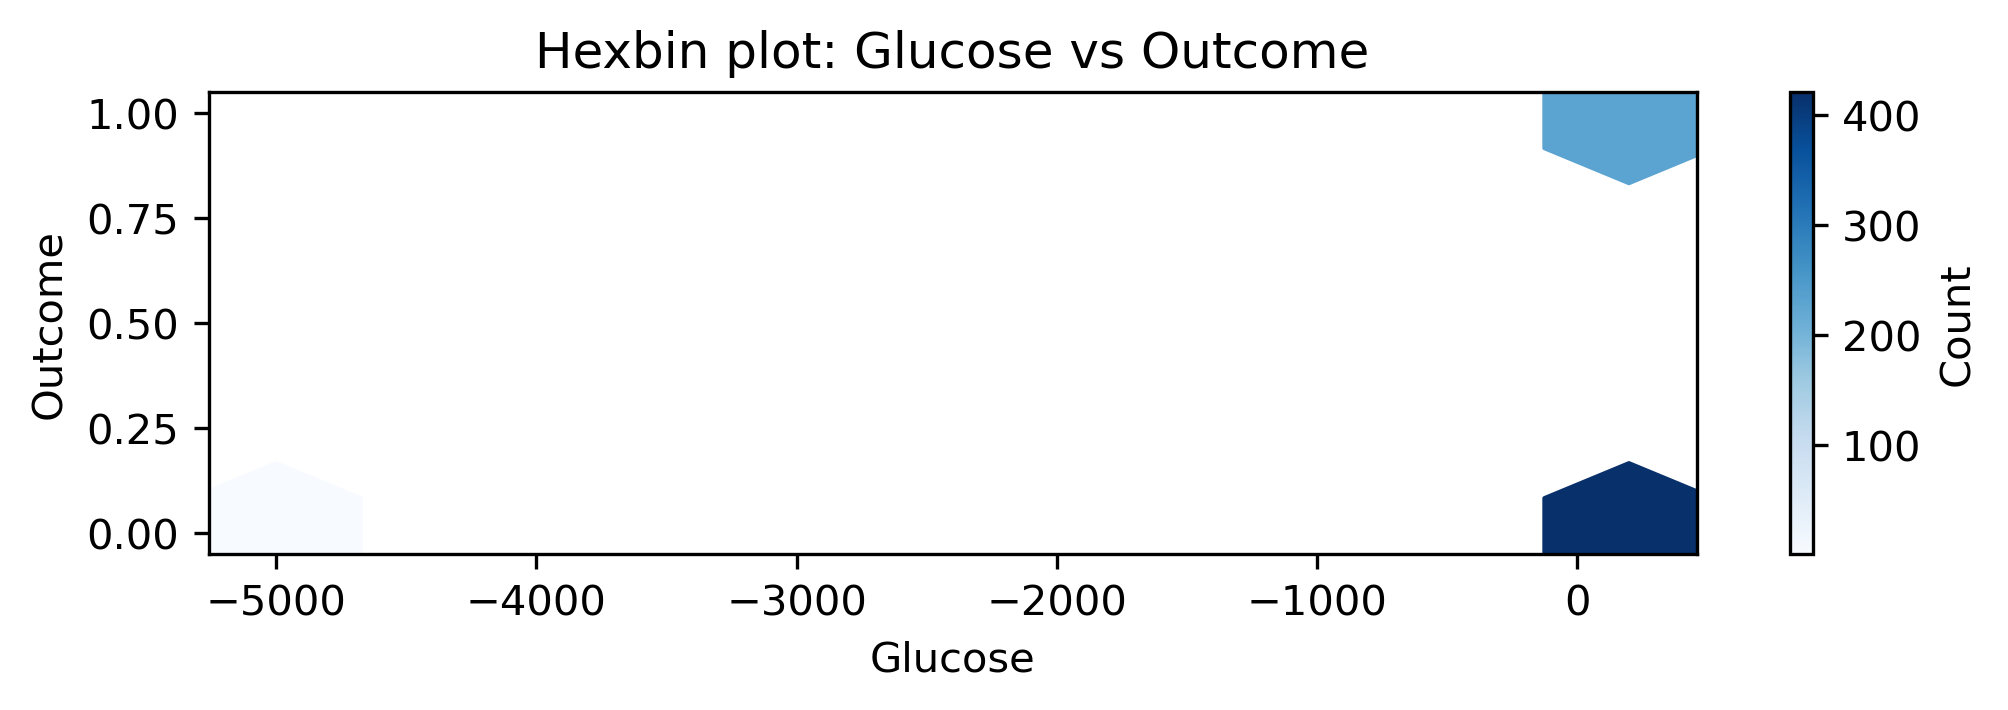
\includegraphics[height=0.15\linewidth]{../HW2_2/Glucose hexbin.png}}
		\subfigure[]{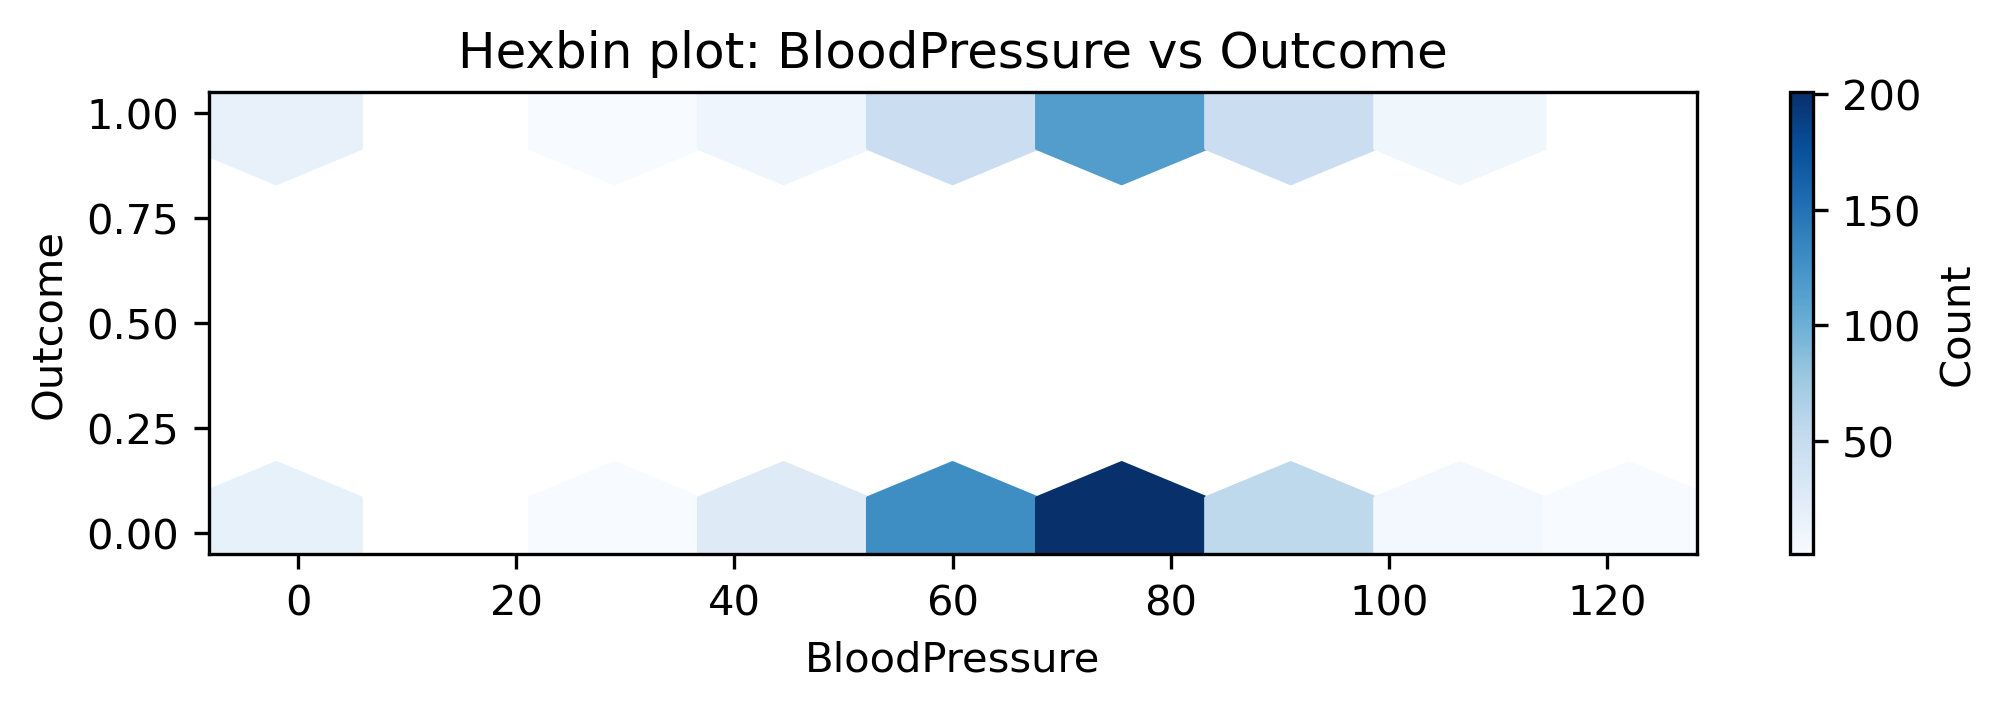
\includegraphics[height=0.15\linewidth]{../HW2_2/BloodPressure hexbin.png}}
		\subfigure[]{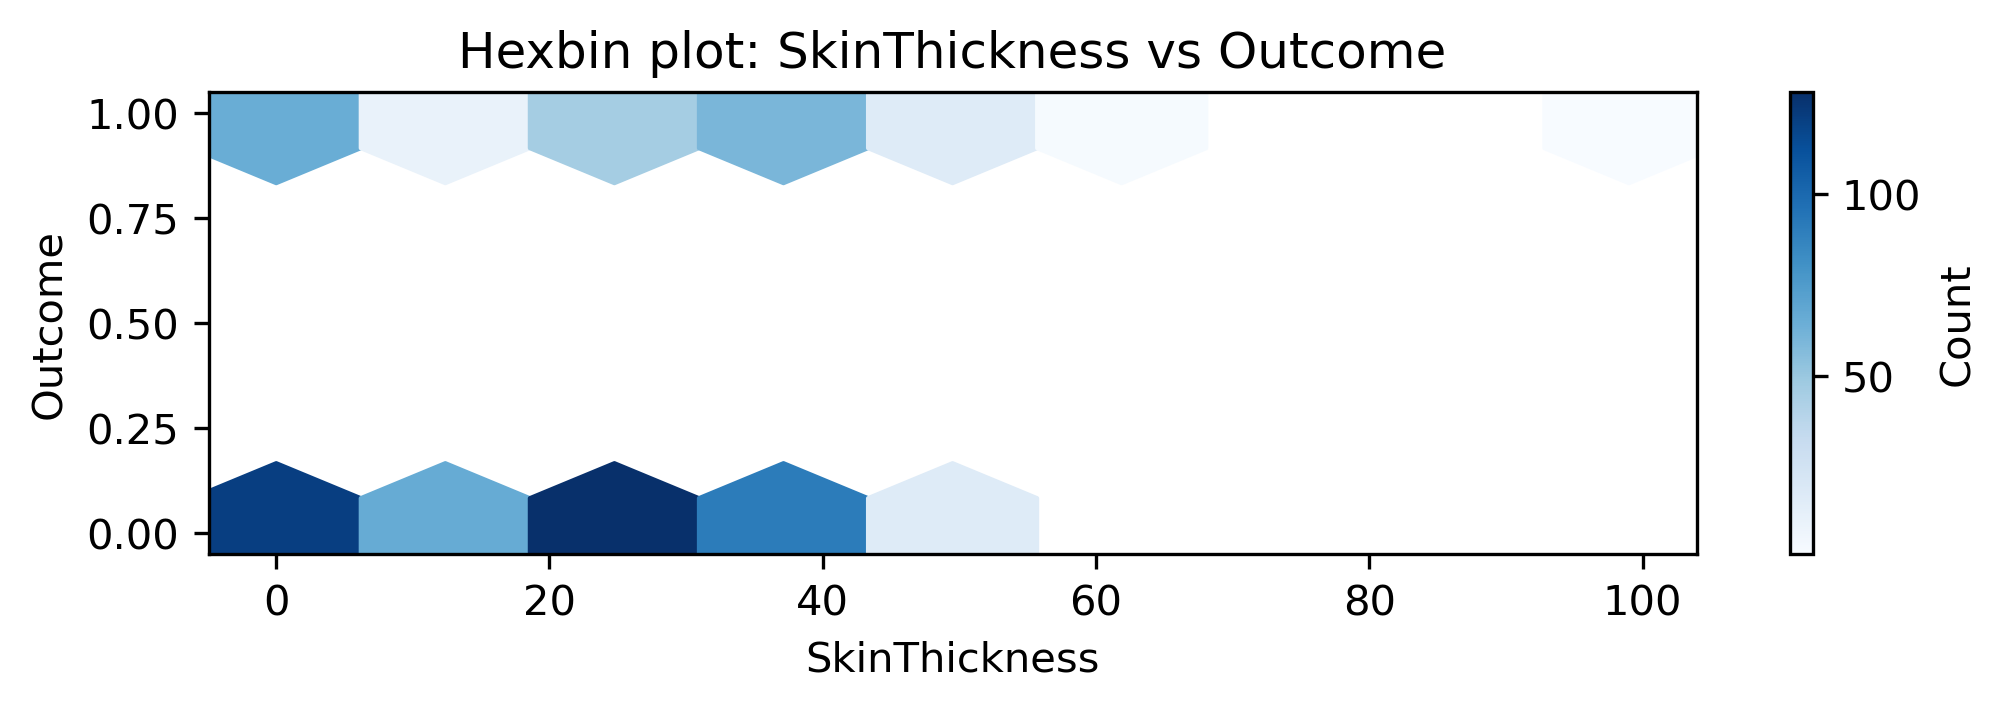
\includegraphics[height=0.15\linewidth]{../HW2_2/SkinThickness hexbin.png}}
		\subfigure[]{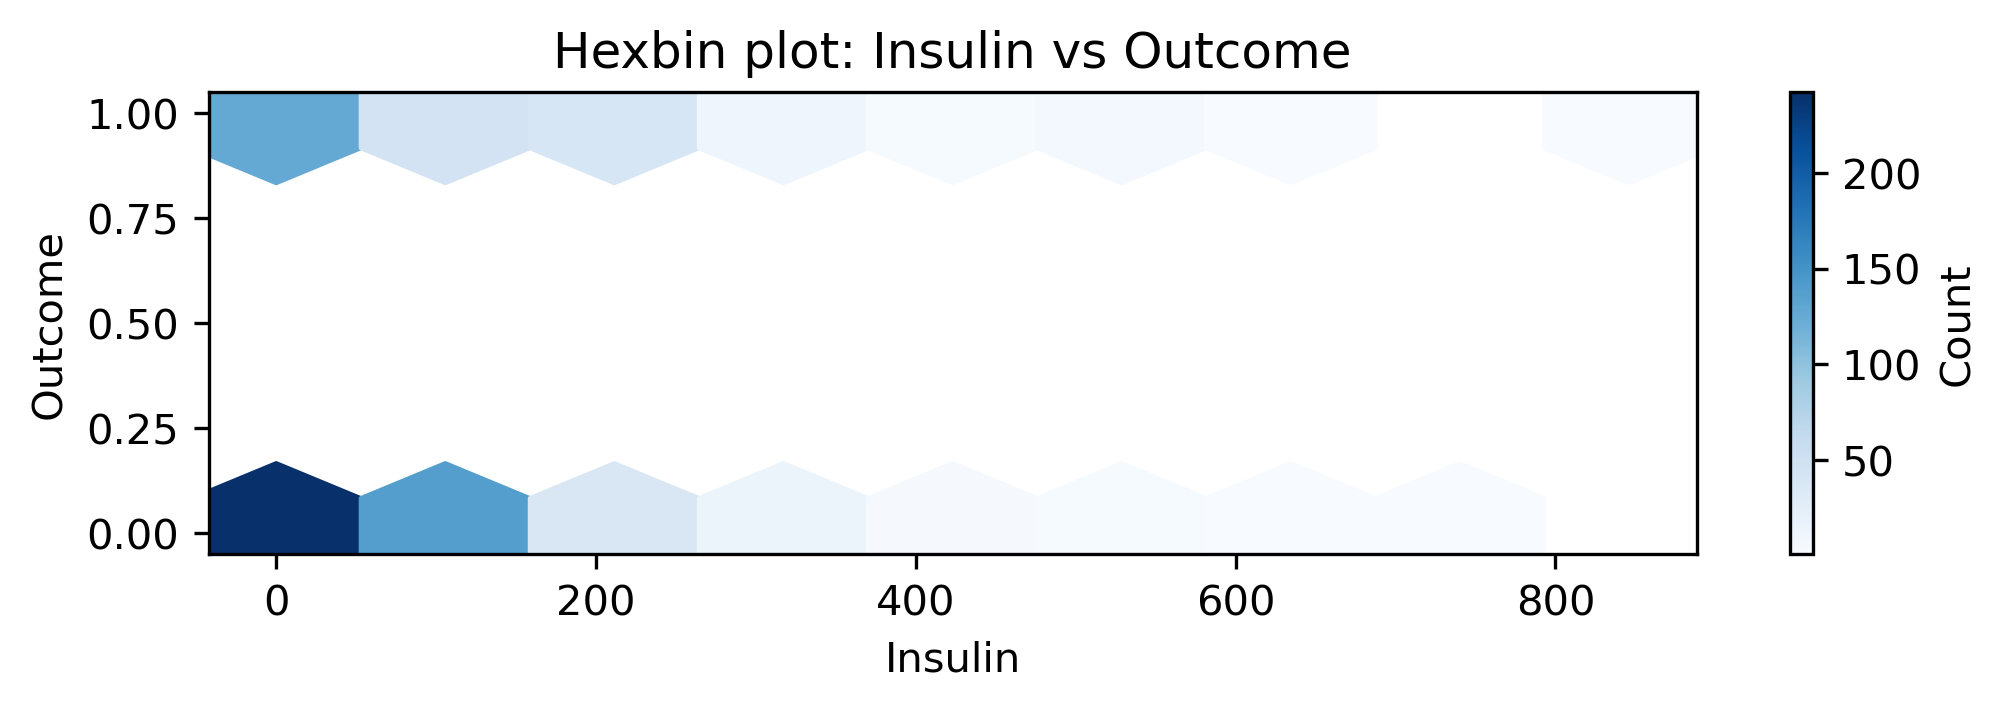
\includegraphics[height=0.15\linewidth]{../HW2_2/Insulin hexbin.png}}
		\subfigure[]{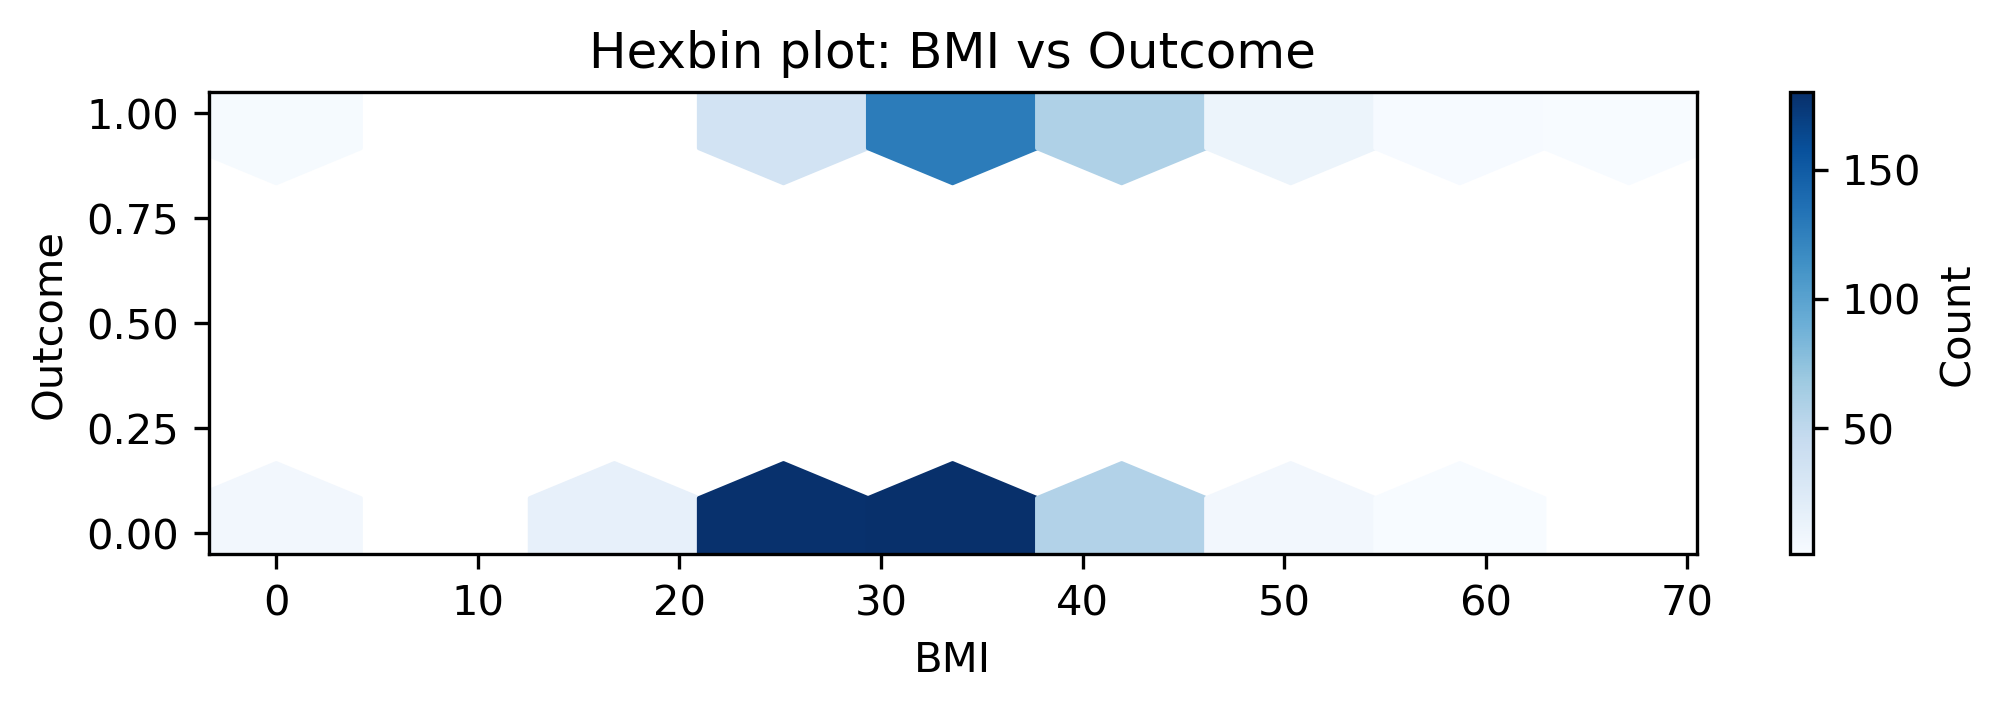
\includegraphics[height=0.15\linewidth]{../HW2_2/BMI hexbin.png}}
		\subfigure[]{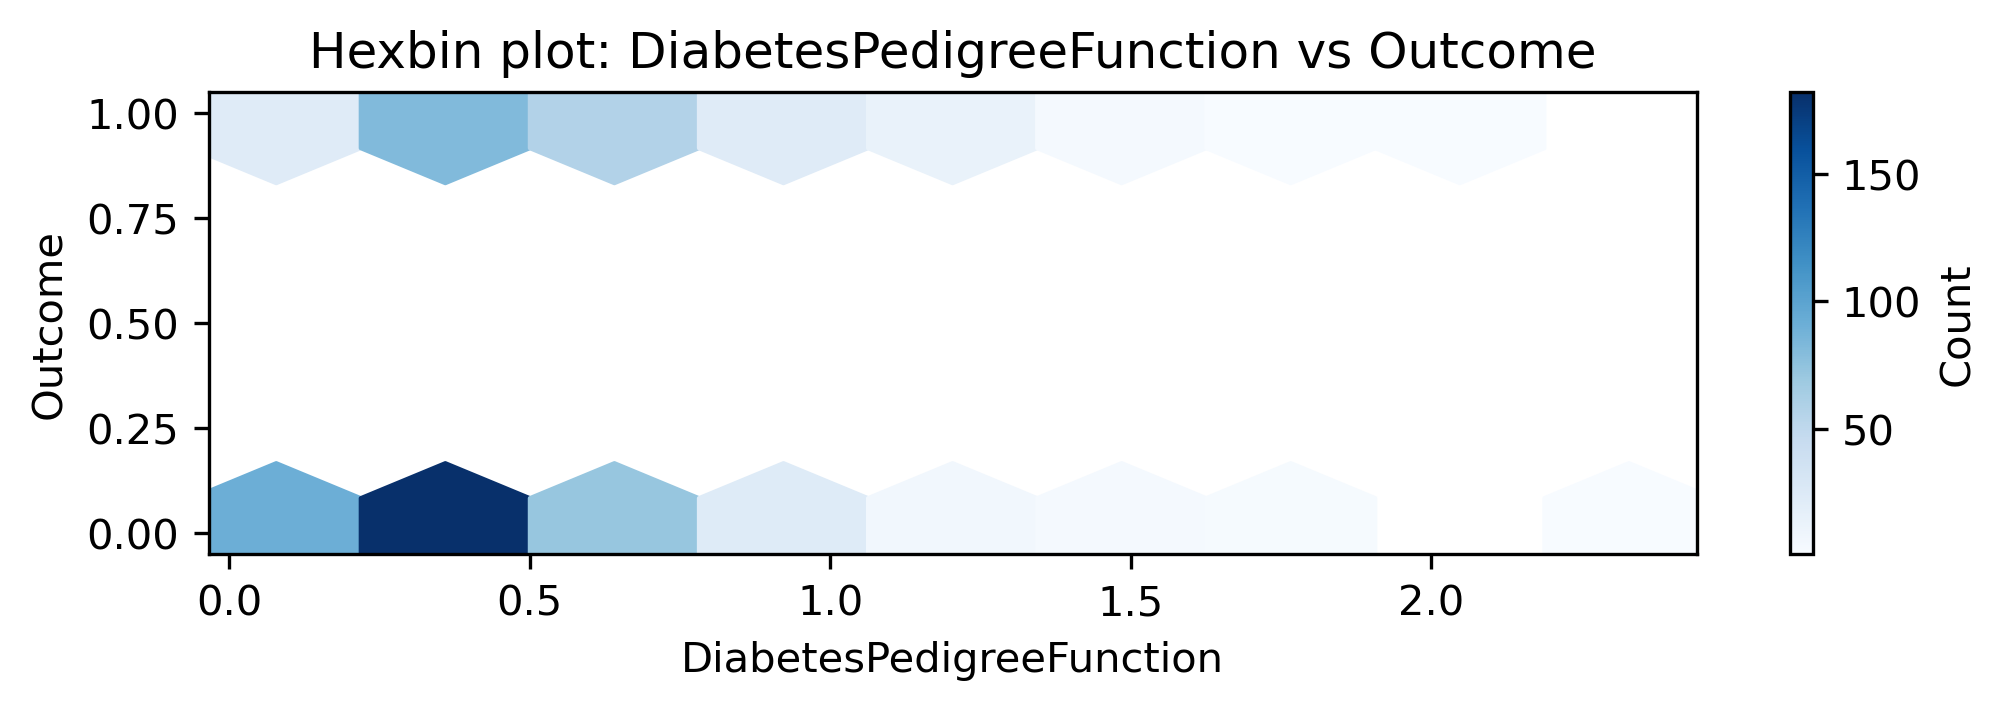
\includegraphics[height=0.15\linewidth]{../HW2_2/DiabetesPedigreeFunction hexbin.png}}
		\subfigure[]{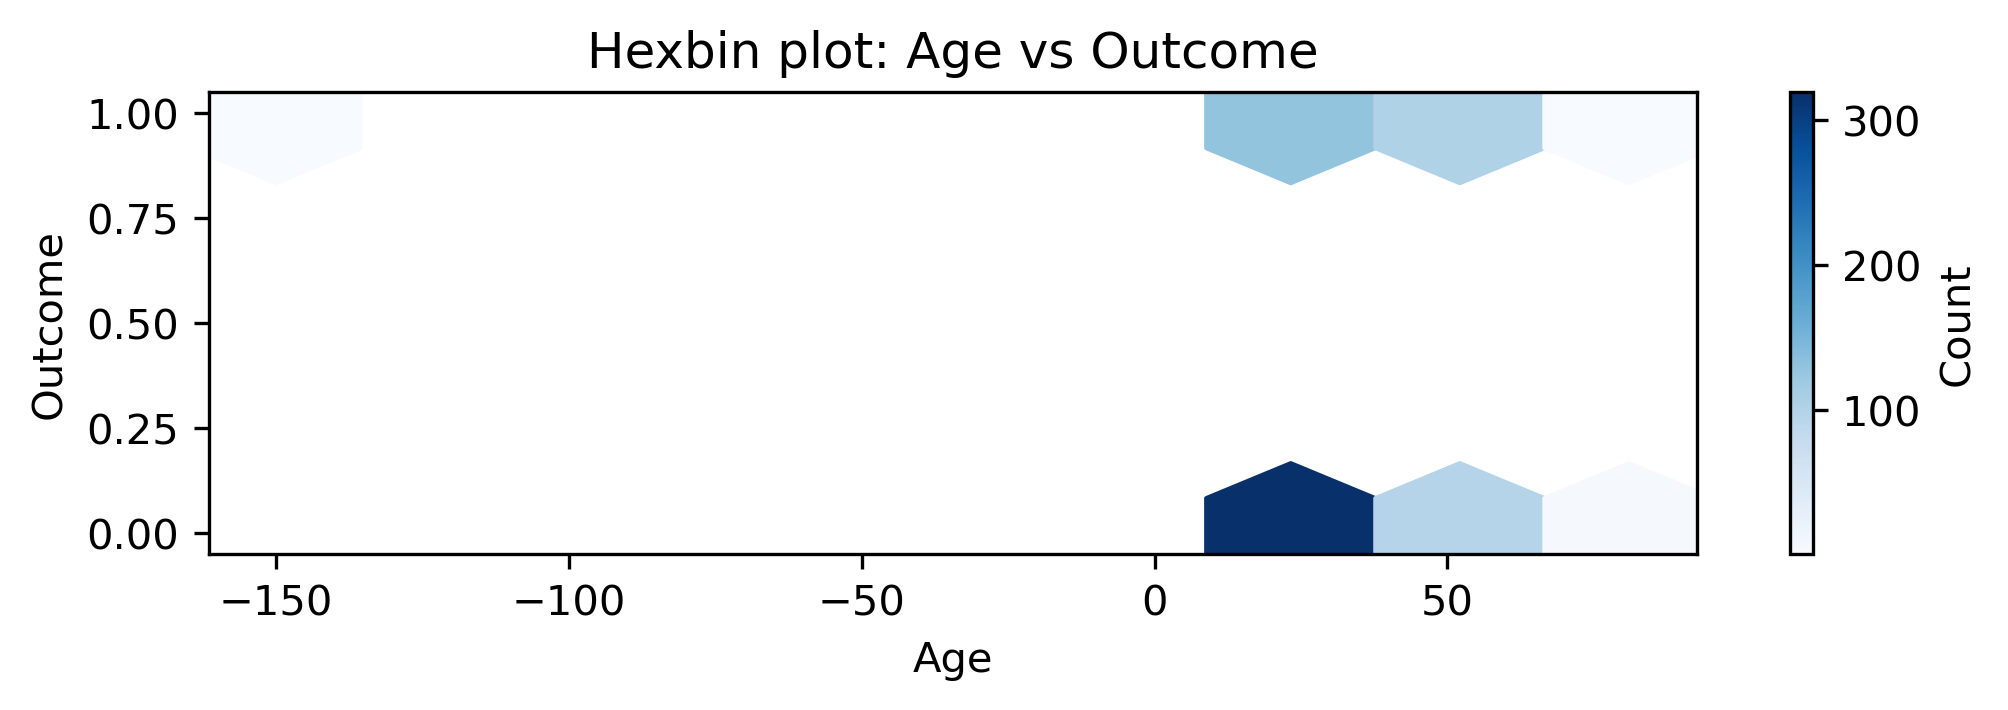
\includegraphics[height=0.15\linewidth]{../HW2_2/Age hexbin.png}}
		\caption{توزیع داده‌های خام به صورت \lr{hexbin}}
		\label{fig:hexbin1}
	\end{figure*}
	
	\subsection{پیش پردازش دادگان}
	به منظور حذف داده‌های پرت، مقدار $IQR$ را حساب می‌کنیم که به زبان ساده اختلاف میان چارک سوم و اول است.
	\begin{equation}
		IQR = Q_3 - Q_1
	\end{equation}
	داده‌هایی که از ۱/۵ برابر این مقدار نسبت به چارک‌های اول و سوم فاصله داشته باشند، حذف خواهند شد. به این ترتیب، توزیع داده‌ها پس از انجام اصلاحات در
	\autoref{fig:hist2}
	در می‌آید. همچنین مقایسه مقدار \lr{skewness} برای قبل و بعد اصلاح داده‌ها در 
	\autoref{tab:skewness}
	آمده است. 
		\begin{figure*}[!h]
		\centering
		\subfigure[]{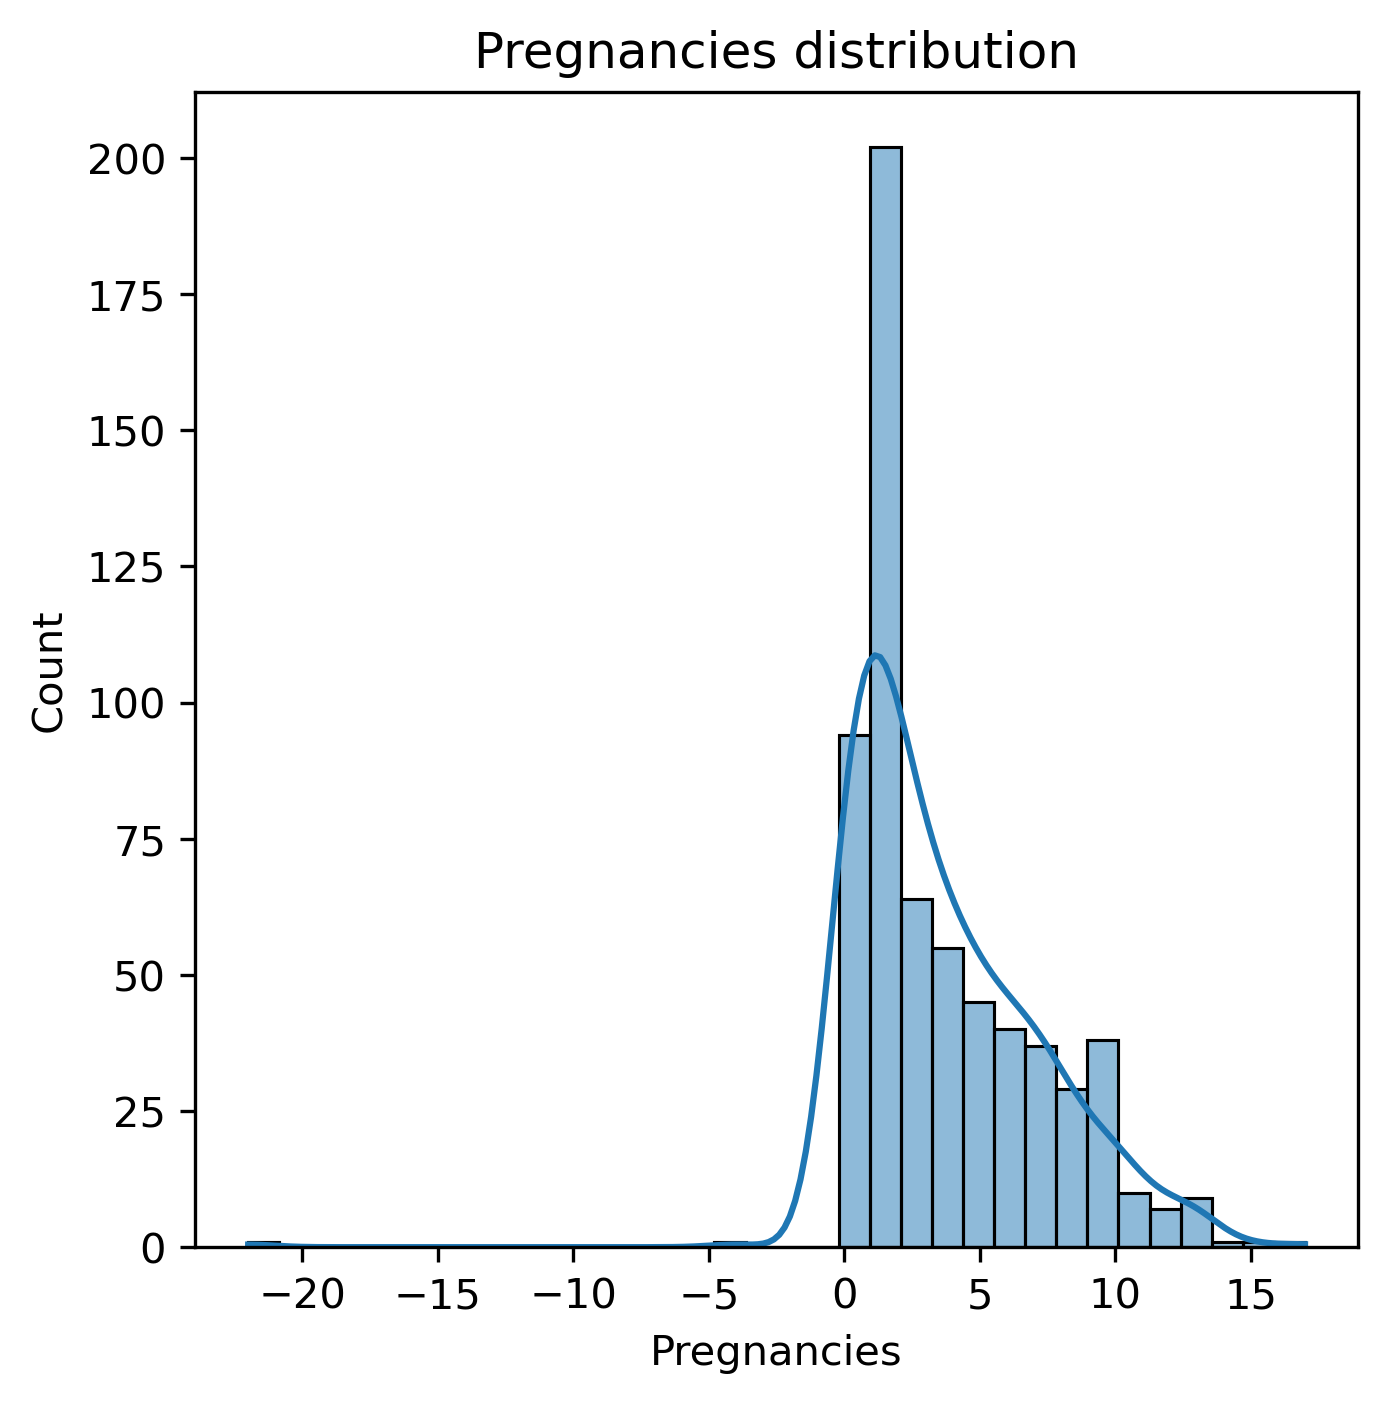
\includegraphics[height=0.31\linewidth]{../HW2_2/Pregnancies distribution.png}}
		\subfigure[]{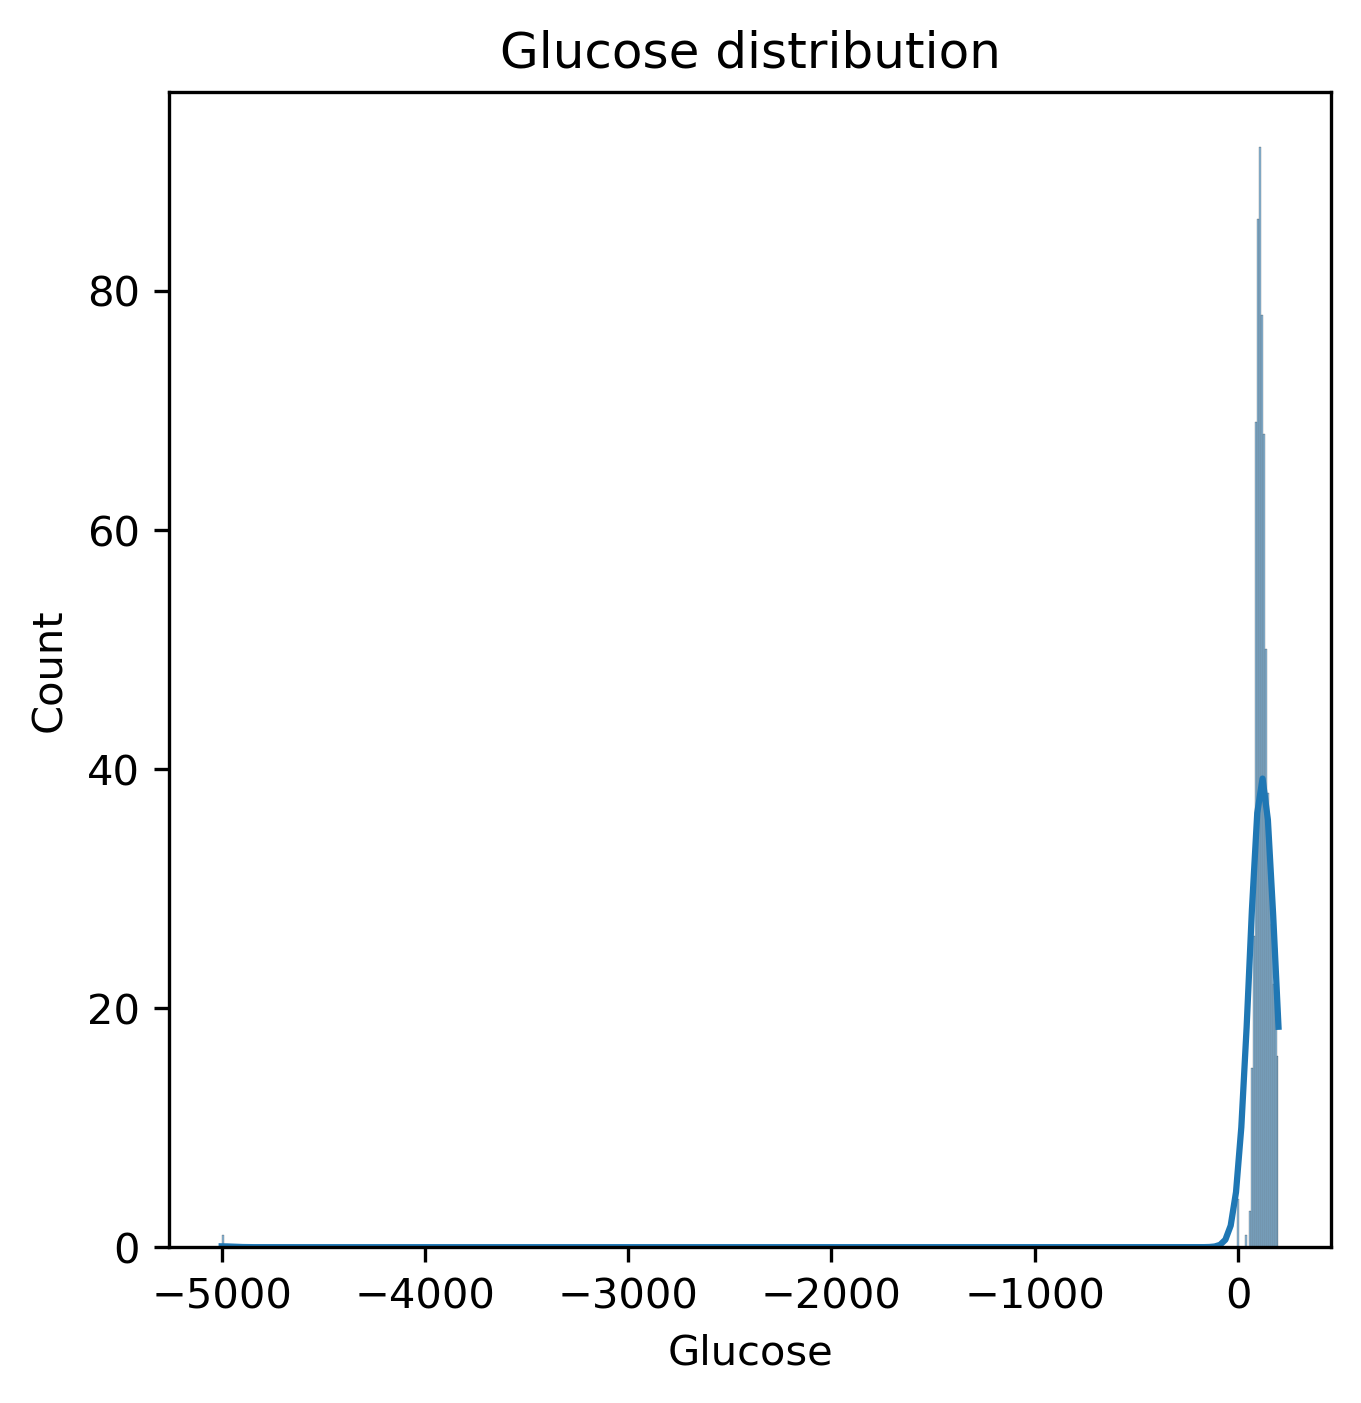
\includegraphics[height=0.31\linewidth]{../HW2_2/Glucose distribution.png}}
		\subfigure[]{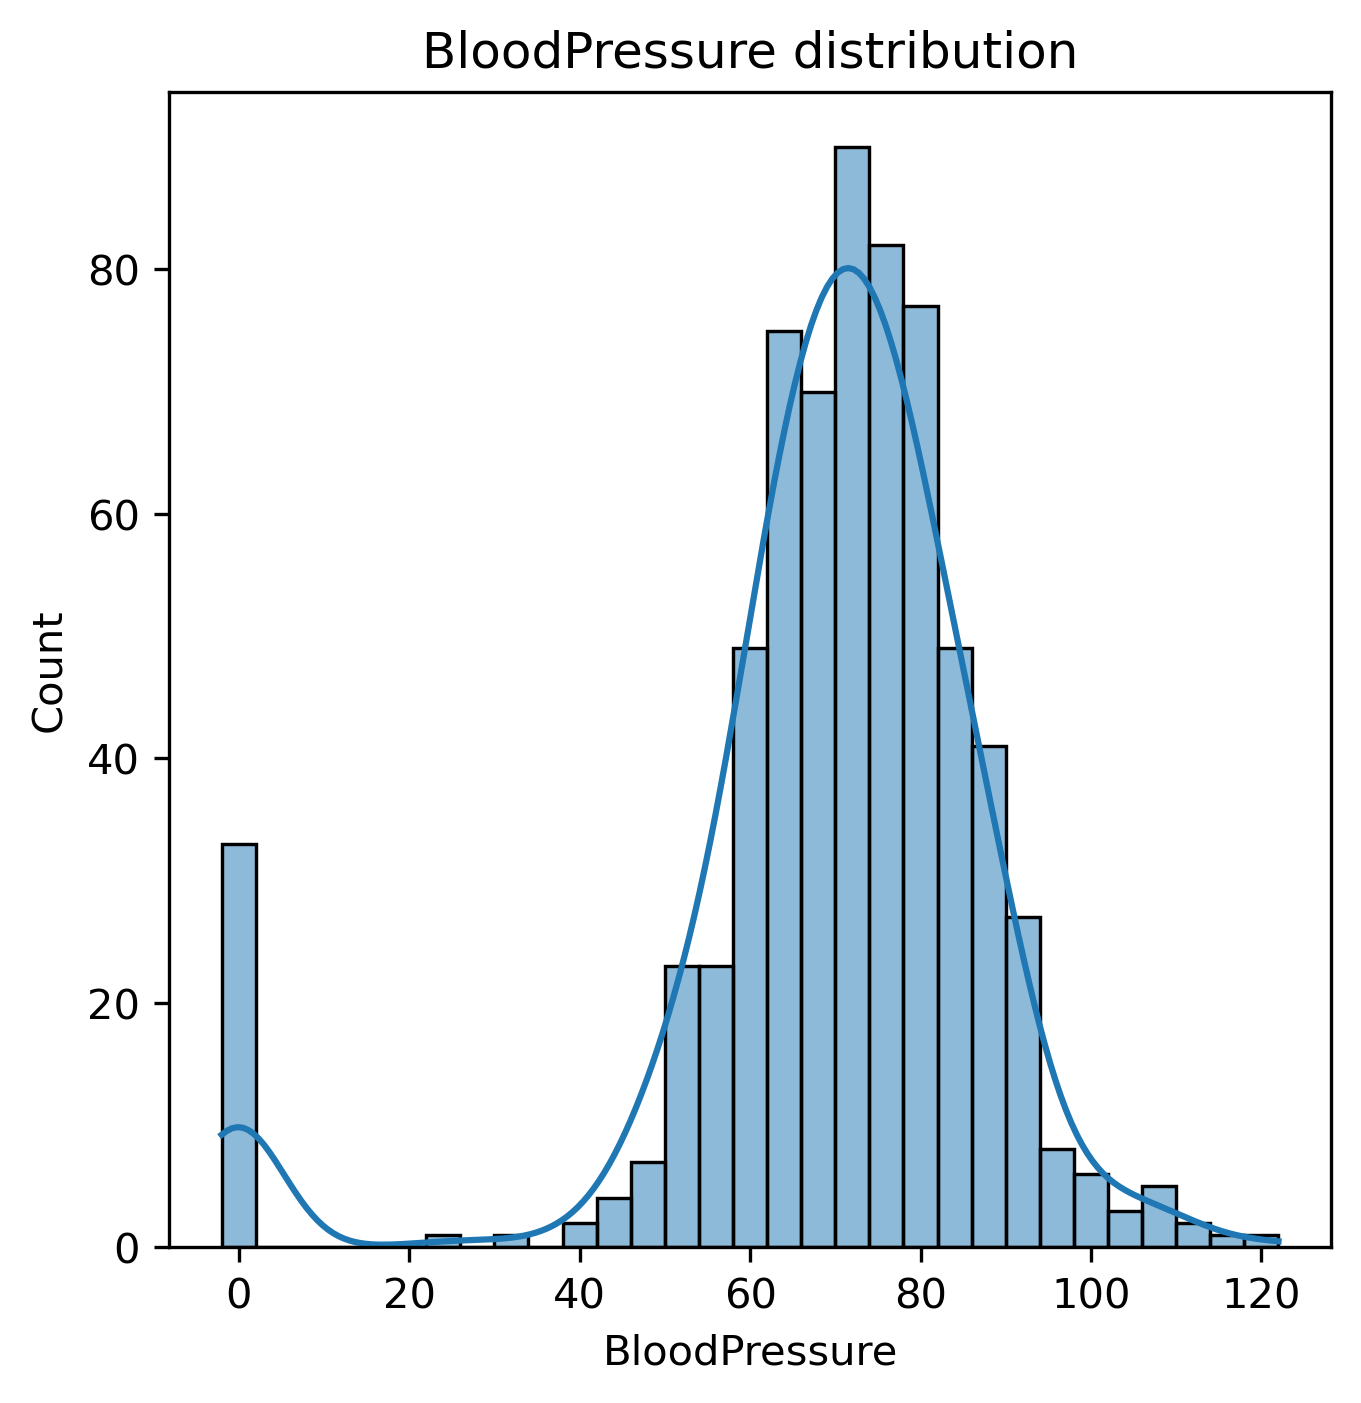
\includegraphics[height=0.31\linewidth]{../HW2_2/BloodPressure distribution.png}}
		\subfigure[]{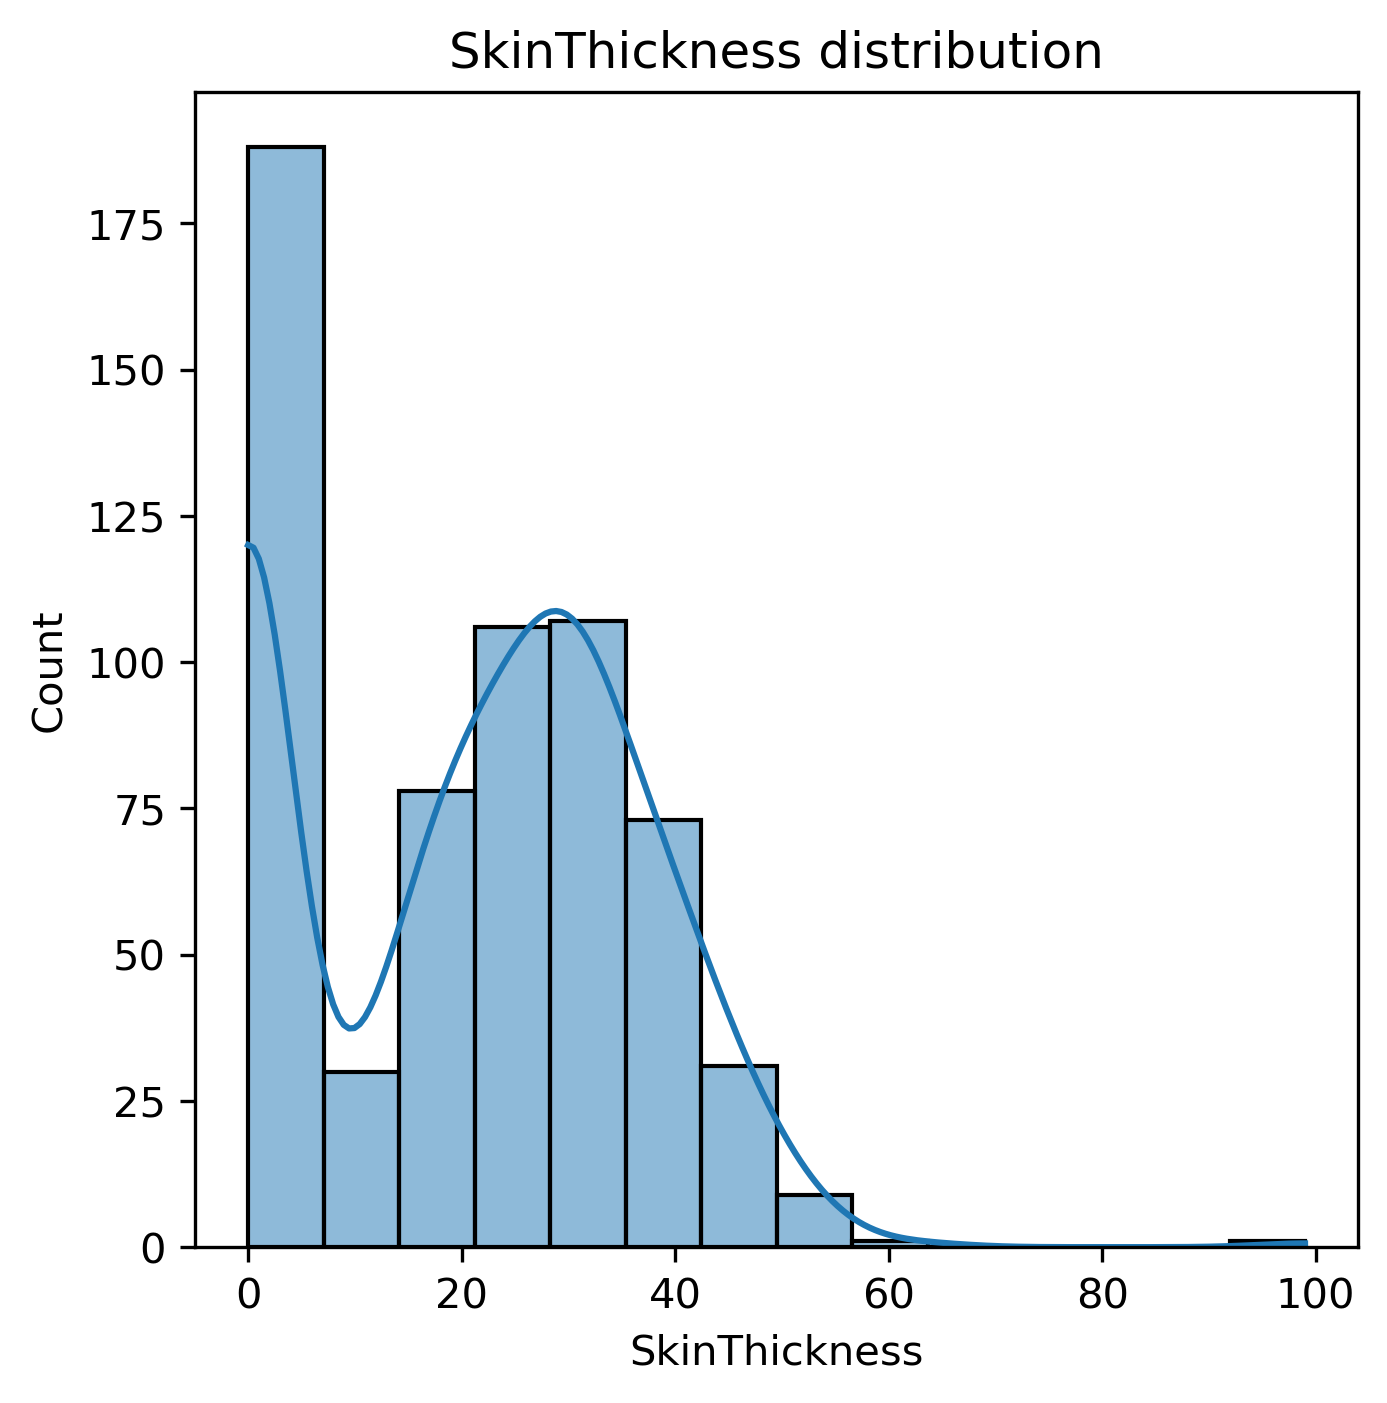
\includegraphics[height=0.31\linewidth]{../HW2_2/SkinThickness distribution.png}}
		\subfigure[]{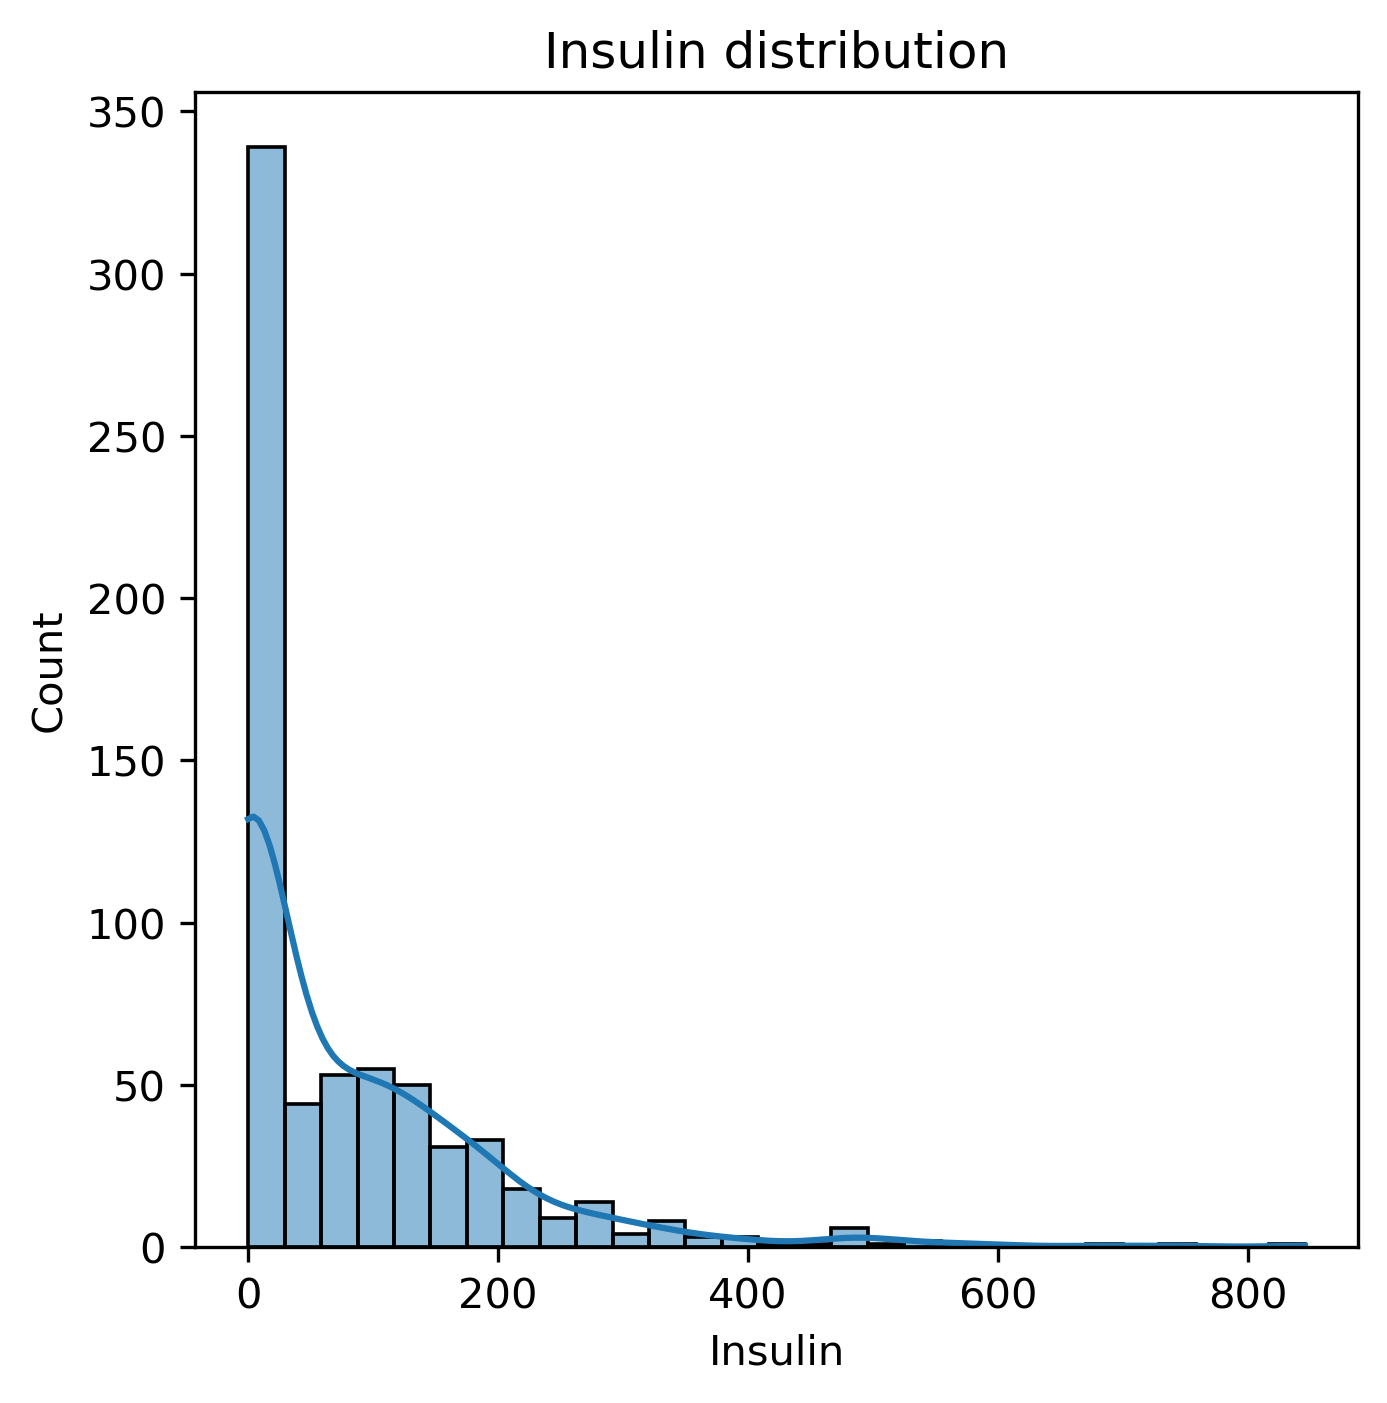
\includegraphics[height=0.31\linewidth]{../HW2_2/Insulin distribution.png}}
		\subfigure[]{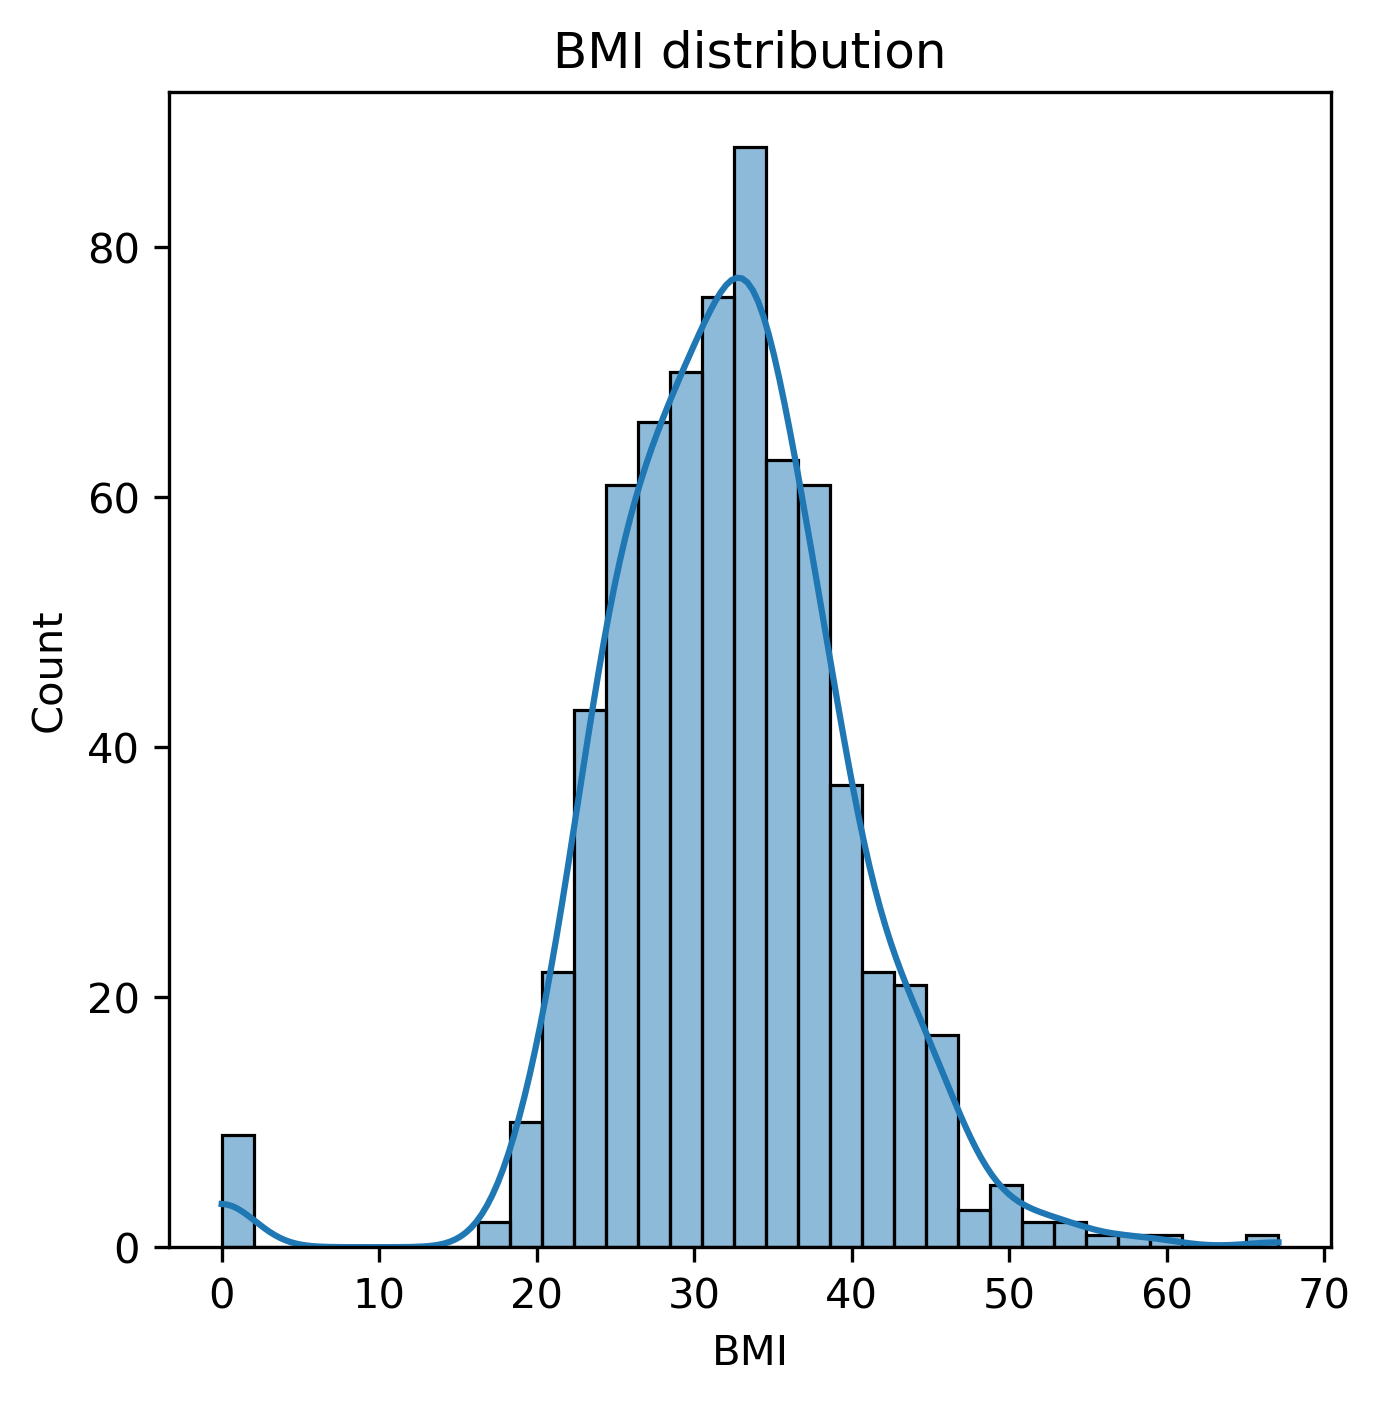
\includegraphics[height=0.31\linewidth]{../HW2_2/BMI distribution.png}}
		\subfigure[]{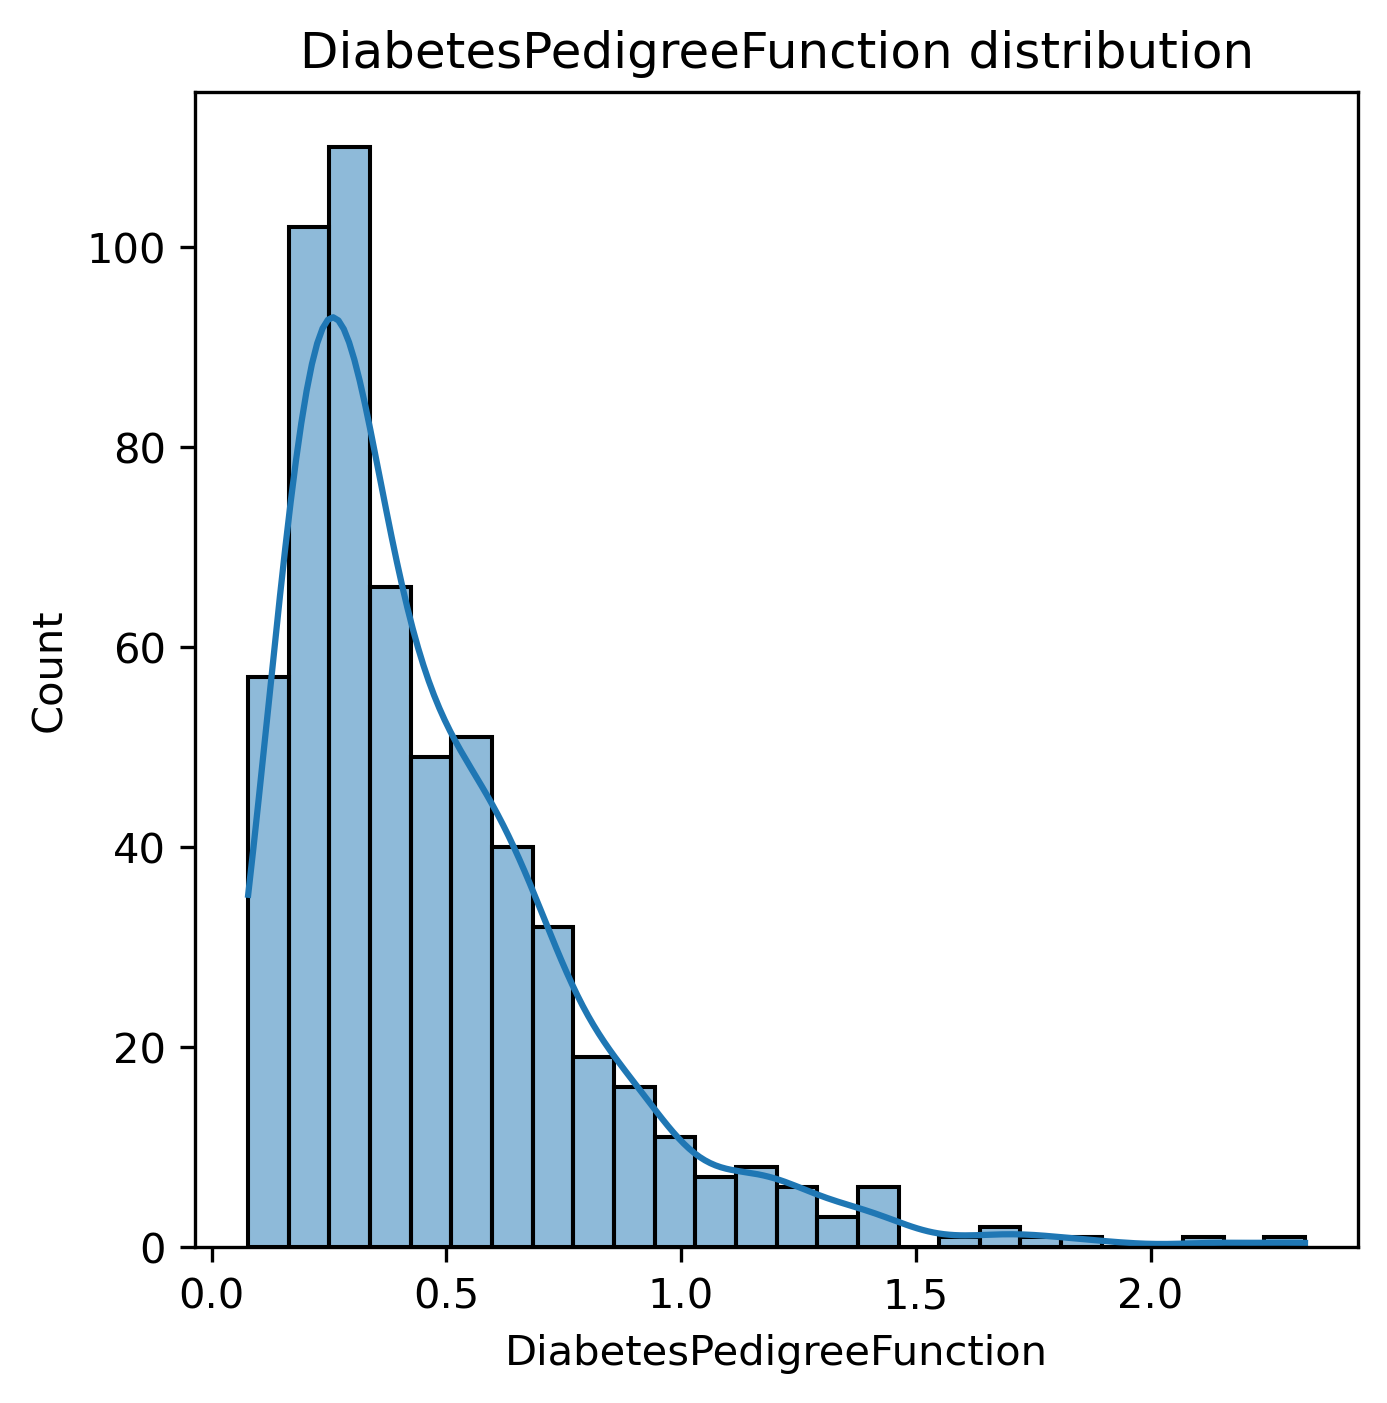
\includegraphics[height=0.31\linewidth]{../HW2_2/DiabetesPedigreeFunction distribution.png}}
		\subfigure[]{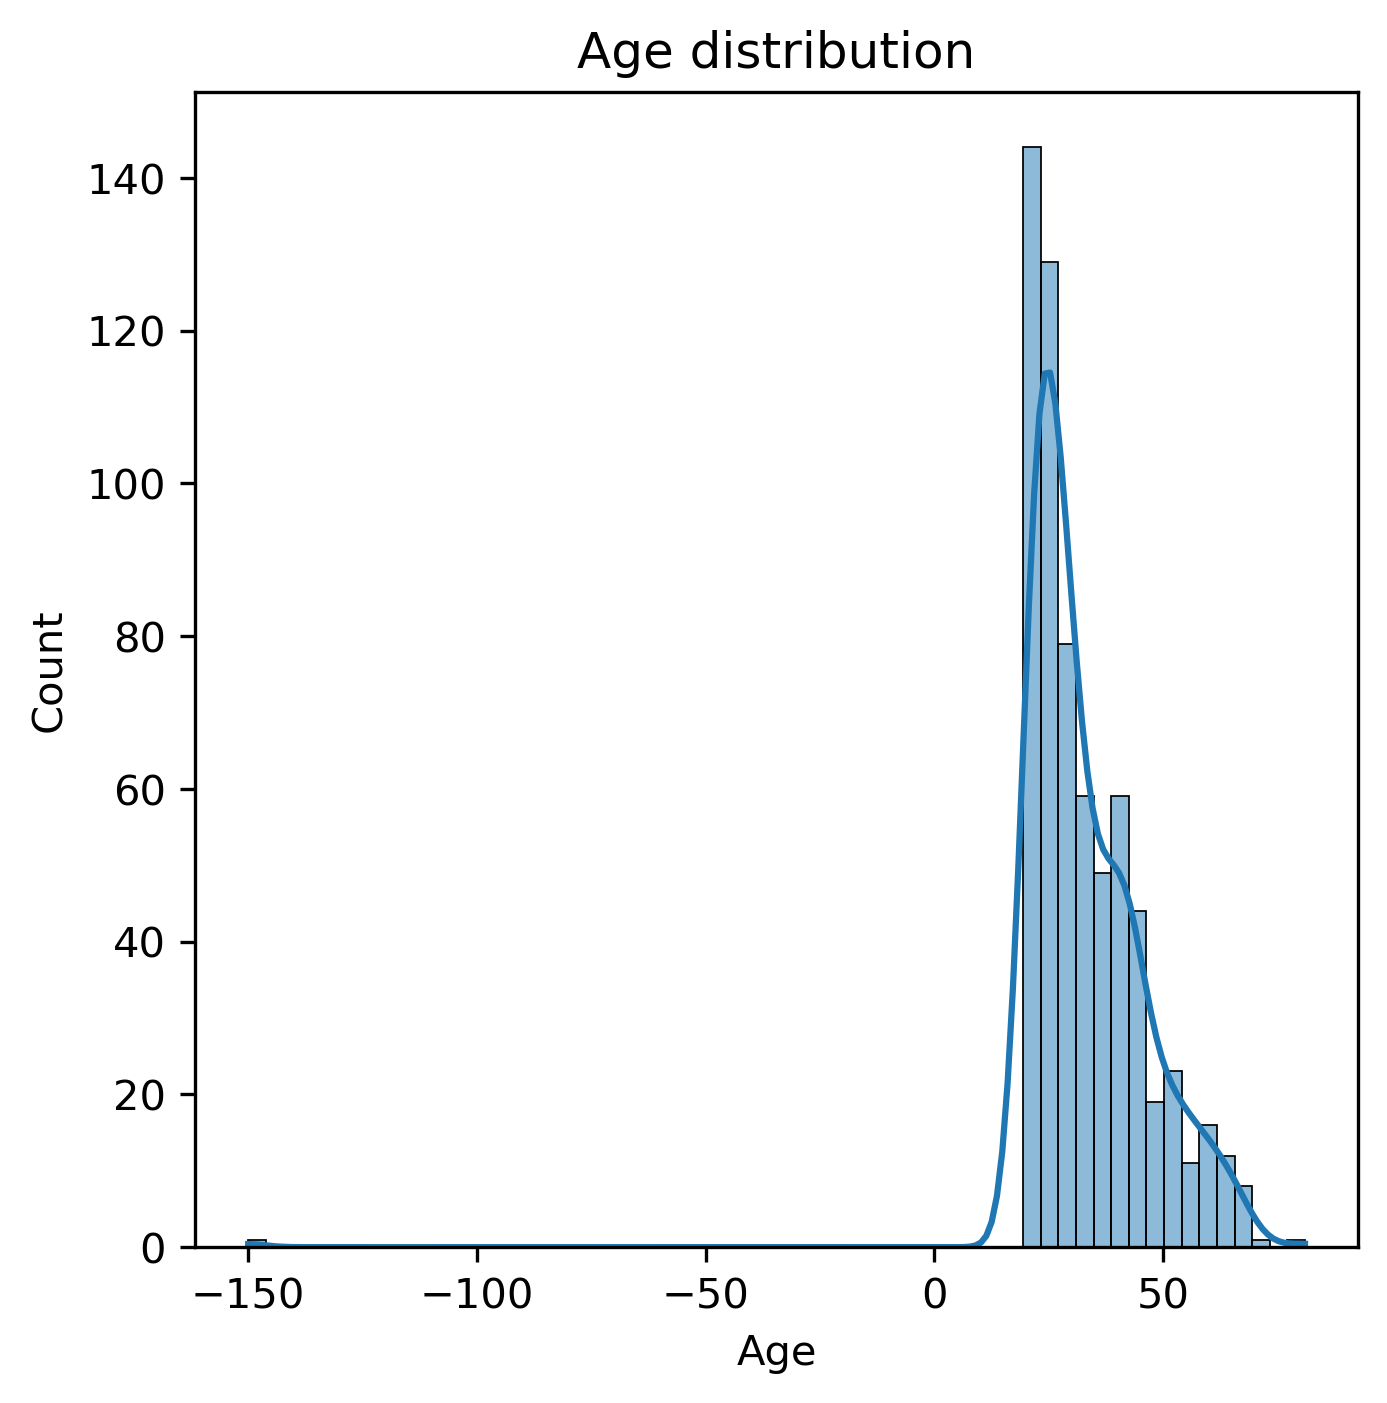
\includegraphics[height=0.31\linewidth]{../HW2_2/Age distribution.png}}
		\caption{توزیع داده‌های اصلاح شده به صورت هیستوگرام}
		\label{fig:hist2}
	\end{figure*}
	
	\begin{table}[h!]
		\centering
		\caption{مقدار \lr{skewness} برای قبل و بعد اصلاح داده‌های پرت}
		\begin{latin}
			{\scriptsize
				\begin{tabular}{lcc}
					\toprule
					Column                     & Skewness (before) & Skewness (after)     \\ 
					\midrule
					Pregnancies                & 0.25119            & 0.85010  \\ 
					Glucose                    & -24.61344            & 0.41643  \\ 
					BloodPressure              & -1.82534             & -0.39650  \\ 
					SkinThickness              & 0.16367            & 0.06288  \\ 
					Insulin                    & 2.30348             & 1.18579  \\ 
					BMI                        & -0.35182             & 0.16488  \\ 
					DiabetesPedigreeFunction   & 1.78627            & 1.00988  \\ 
					Age                        & -2.83221            & 0.98922  \\
					\bottomrule
				\end{tabular}
			}
		\end{latin}
		\label{tab:skewness}
	\end{table}
	سپس مقادیر ناموجود با میانگین مقادیر جابه‌جا می‌شوند. همچنین از جایی که مقادیر منفی صحیح نمی‌باشند، به مقادیر منفی نیز مقادیر میانگین نسبت داده می‌شود تا دقت نهایی مدل بالا رود.\\
	فرایند 
	\lr{Normalize}
	کردن داده‌ها بازه داده‌ها را به $[0,1]$ یا $[-1,1]$ تغییر می‌دهد و برای داده‌هایی به کار می‌روند که توزیع گاوسی ندارند. فرایند 
	\lr{Standardize}
	داده‌ها را به صورتی تغییر می‌دهد که میانگین داده‌ها صفر و انجراف معیار داده‌ها یک شود. از جایی که داده‌های به صورت کلی توزیع گاوسی ندارند داده‌ها را
	\lr{Normalize}
	می‌کنیم
	\clearpage
	\subsection{انتخاب، آموزش و ارزیابی مدل}
	با تقسیم داده‌های به صورت ۸۰ ۲۰، مدل‌های زیر برای پیش‌بینی پیاده‌سازی شده‌اند. برای هر کدام از مدل‌ها دو پارامتر (برای \lr{KNN} یک پارامتر) به وسیله 
	\verb|GridSearchCV|
	تغییر داده شده‌اند تا پارامتر‌های بهینه استخراج شوند.
	\subsection{\lr{Logistic Regression}}
		این مدل دارای پارامترهای زیر بوده است:
		$$C = 10$$
		$$solver = 'liblinear'$$
		پارامتر همسان سازی $C$ به طور کلی تعادلی میان خطای تربیت پایین و خطای آزمون پایین برقرار می‌کند. به این ترتیب پارامتر همسان‌سازی بالا میزان اورفیت را کاهش می‌دهد اما به طور کلی بایاس مدل را زیاد می‌کند. حل‌‌گر مدل از میا‌ن چند الگوریتم انتخاب شده تا الگوریتم بهتر انتخاب شود.\\
		نتایج تربیت و آزمون مدل به صورت خلاصه در جدول زیر آمده است:
		\begin{table}[h!]
			\caption{دقت مدل \lr{Logistic Regression}}
			\begin{latin}
				\centering
				\begin{tabular}{|l|c|c|}
					\hline
					\textbf{Model} & \textbf{Test precision} & \textbf{Test accuracy} \\ \hline
					Logistic Regression & 0.70454 & 0.75974 \\ \hline
				\end{tabular}
			\end{latin}
			\label{tab:logisticregression_results}
		\end{table}
		\begin{figure}[!h]
			\centerline{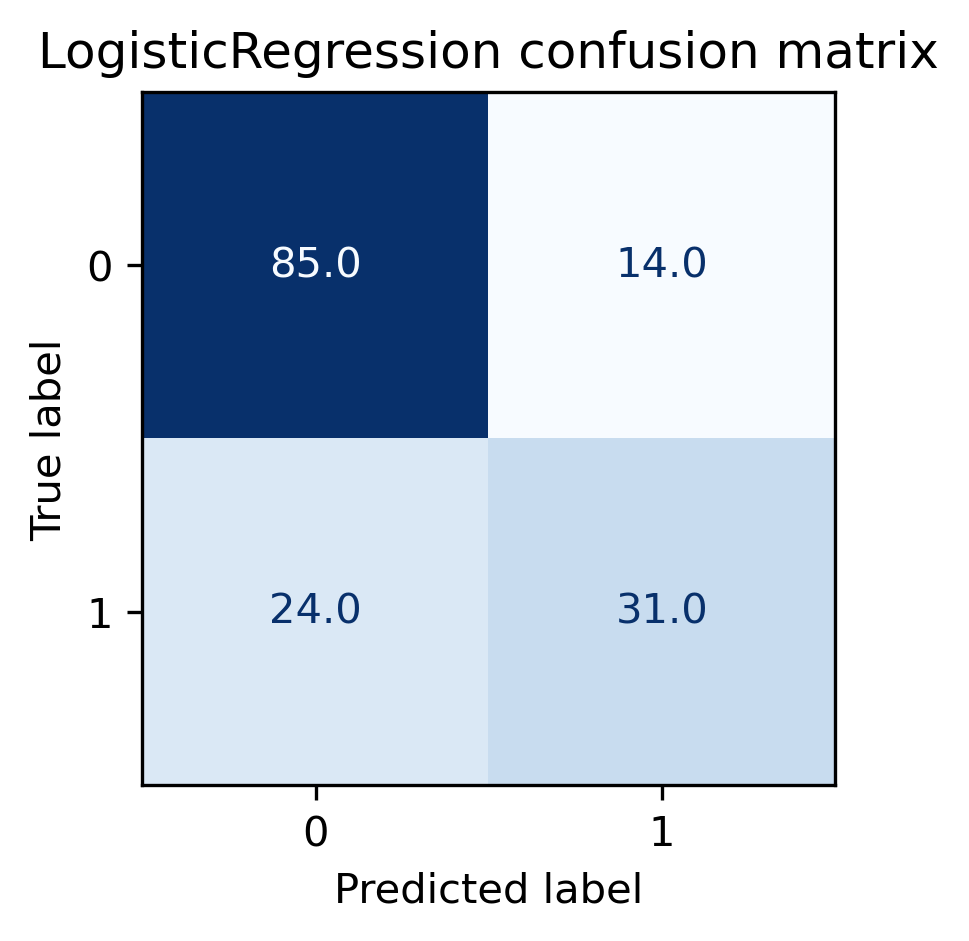
\includegraphics[width=0.5\linewidth]{../HW2_2/LogisticRegression confusion.png}}
			\caption{ماتریس سردرگمی برای مدل \lr{Logistic Regression}}
			\label{fig:confusion_logistic}
		\end{figure}
		\pagebreak
		\subsection{\lr{K-Nearest-Neighbor}}
		این مدل دارای پارامتر زیر بوده است:
		$$K = 11$$
		تعداد همسایه‌ها چنانجه کم باشد، مدل را اورفیت می‌کند و زیاد بودن آن باعث آندرفیت شدن آن می‌شود. بنابراین تعیین مقدار بهینه حائز اهمیت است.\\
		نتایج تربیت و آزمون مدل به صورت خلاصه در جدول زیر آمده است:
				\begin{table}[h!]
			\caption{دقت مدل \lr{K Nearest Neighbor}}
			\begin{latin}
				\centering
				\begin{tabular}{|l|c|c|}
					\hline
					\textbf{Model} & \textbf{Test precision} & \textbf{Test accuracy} \\ \hline
					K Nearest Neighbor & 0.65517 & 0.70129 \\ \hline
				\end{tabular}
			\end{latin}
			\label{tab:knn_results}
		\end{table}
		\begin{figure}[!h]
			\centerline{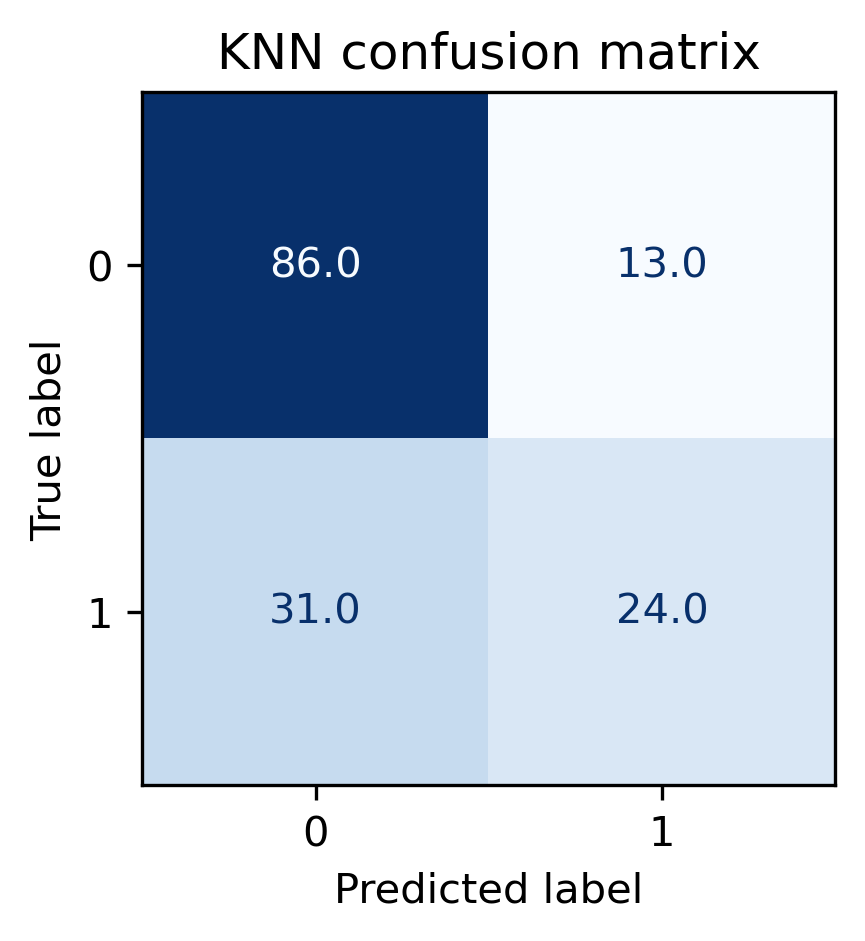
\includegraphics[width=0.5\linewidth]{../HW2_2/KNN confusion.png}}
			\caption{ماتریس سردرگمی برای مدل \lr{K Nearest Neighbor}}
			\label{fig:confusion_knn}
		\end{figure}
		\pagebreak
		\subsection{\lr{Decision Tree}}
		این مدل دارای این مدل دارای پارامترهای زیر بوده است:
		$$max_depth = 10$$
		$$min_samples_split = 10$$
		با تعیین یک عمق مناسب برای درخت تصمیم‌گیری، می‌توان از پیچیدگی مدل و در نهایت اورفیت شدن آن جلوگیری کرد. همجنین مقدار حداقل سمپل‌ها برای شاخه‌ها تعیین می‌کند که مدل تعمیم‌پذیری بالاتری برای داده‌های تست داشته باشد.\\
		نتایج تربیت و آزمون مدل به صورت خلاصه در جدول زیر آمده است:
		\begin{table}[h!]
			\caption{دقت مدل \lr{Decision Tree}}
			\begin{latin}
				\centering
				\begin{tabular}{|l|c|c|}
					\hline
					\textbf{Model} & \textbf{Test precision} & \textbf{Test accuracy} \\ \hline
					Decision Tree & 0.66666 & 0.74675 \\ \hline
				\end{tabular}
			\end{latin}
			\label{tab:decisiontree_results}
		\end{table}
		\begin{figure}[!h]
			\centerline{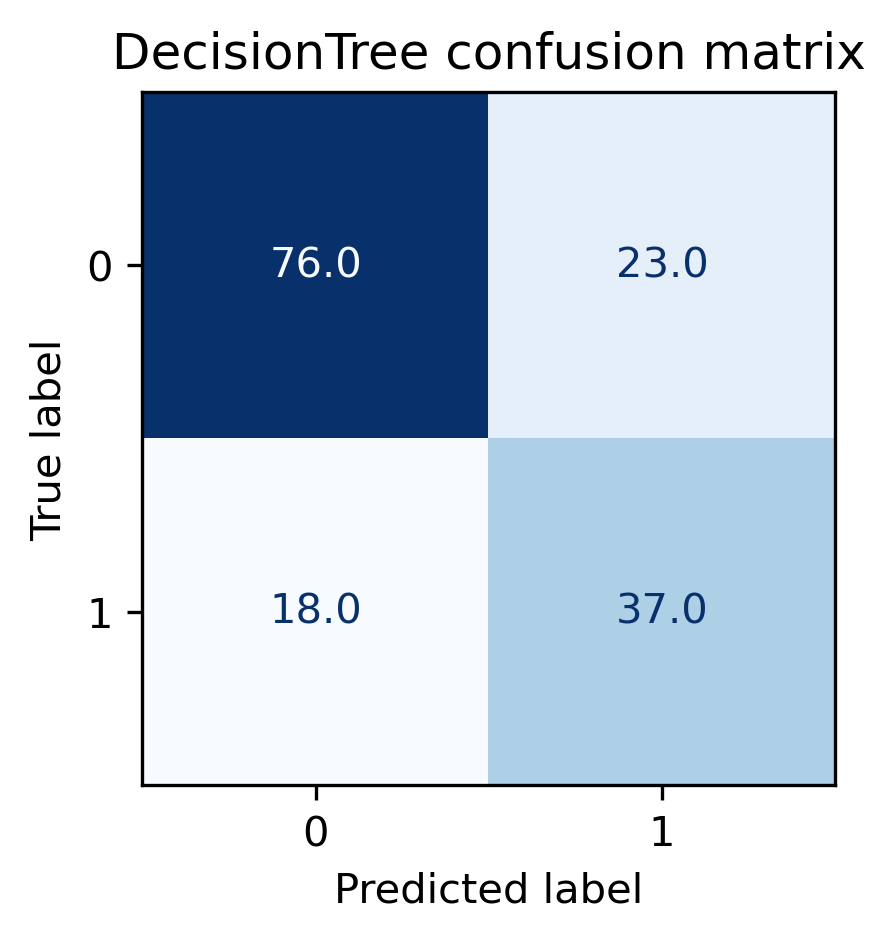
\includegraphics[width=0.5\linewidth]{../HW2_2/DecisionTree confusion.png}}
			\caption{ماتریس سردرگمی برای مدل \lr{Decision Tree}}
			\label{fig:confusion_decisiontree}
		\end{figure}
		\pagebreak
		\subsection{\lr{Random Forest}}
				این مدل دارای پارامترهای زیر بوده است:
		$$max_features = 'sqrt'$$
		$$n_estimators = 100$$
		تعداد ویژگی‌ها در اورفیت و آندرفیت شدن مدل تاثیر خواهد داشت. به این ترتیب کم‌تر کردن ویژگی‌ها از اورفیت شدن جلو‌گیری کرده اما اگر این مقدار خیلی کوچک شود، مدل آندرفیت خواهد بود. در این جا جذر تعداد ویژگی‌ها انتخاب شده است. همچنین تعداد درخت‌ها معمولا در عملکرد مدل تاثیر مثبت دارد اما هزینه محاسباتی بالاتری دارد.\\
		نتایج تربیت و آزمون مدل به صورت خلاصه در جدول زیر آمده است:
				\begin{table}[h!]
			\caption{دقت مدل \lr{Random Forest}}
			\begin{latin}
				\centering
				\begin{tabular}{|l|c|c|}
					\hline
					\textbf{Model} & \textbf{Test precision} & \textbf{Test accuracy} \\ \hline
					Random Forest & 0.67272 & 0.76623 \\ \hline
				\end{tabular}
			\end{latin}
			\label{tab:randomforest_results}
		\end{table}
		\begin{figure}[!h]
			\centerline{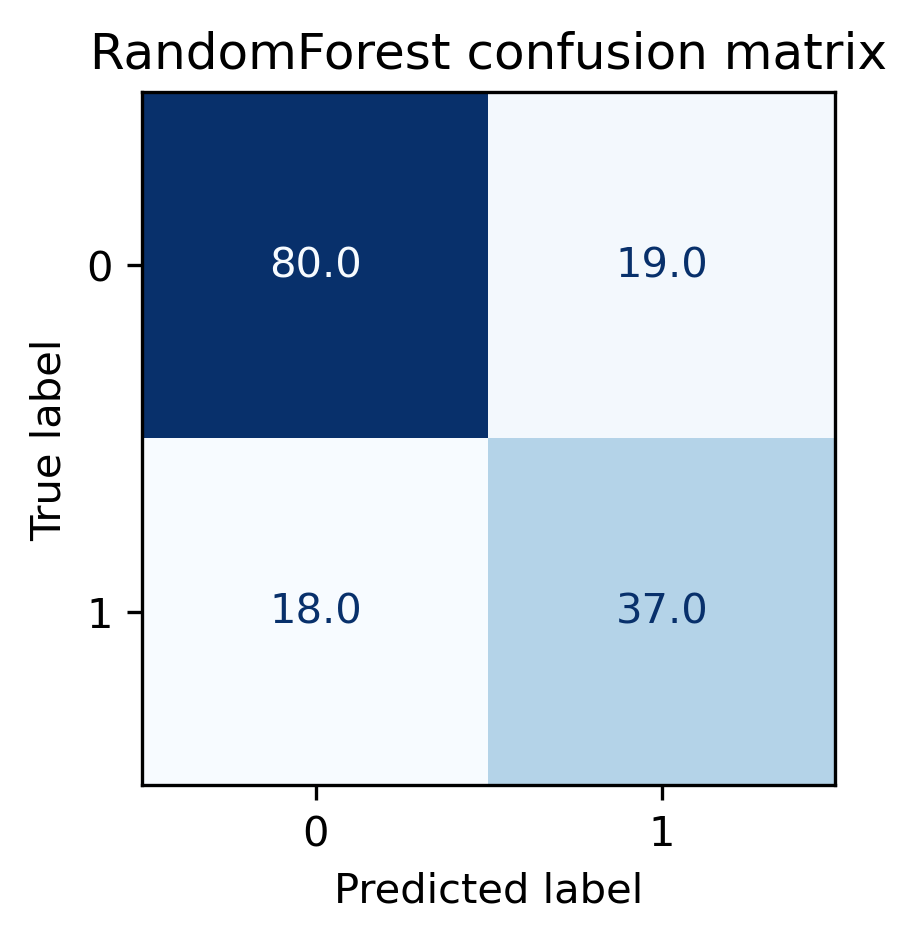
\includegraphics[width=0.5\linewidth]{../HW2_2/RandomForest confusion.png}}
			\caption{ماتریس سردرگمی برای مدل \lr{Random Forest}}
			\label{fig:confusion_randomforest}
		\end{figure}
		\pagebreak
		\subsection{\lr{Support Vector Machine}}
				این مدل دارای پارامترهای زیر بوده است:
		$$C = 1$$
		$$gamma = 1e-4$$
		پارامتر همسان سازی $C$ به طور کلی تعادلی میان خطای تربیت پایین و خطای آزمون پایین برقرار می‌کند. به این ترتیب پارامتر همسان‌سازی بالا میزان اورفیت را کاهش می‌دهد اما به طور کلی بایاس مدل را زیاد می‌کند. پارامتر گاما به طور کلی نشان‌گر میزان تاثیر هر یک از داده‌ها بر روی فرایند تمرین است.\\
		نتایج تربیت و آزمون مدل به صورت خلاصه در جدول زیر آمده است:
		\begin{table}[h!]
		\caption{دقت مدل \lr{Support Vector Machine}}
			\begin{latin}
				\centering
				\begin{tabular}{|l|c|c|}
					\hline
					\textbf{Model} & \textbf{Test precision} & \textbf{Test accuracy} \\ \hline
					Support Vector Machine & 0.75609 & 0.77922 \\ \hline
				\end{tabular}
			\end{latin}
			\label{tab:svm_results}
		\end{table}
		\begin{figure}[!h]
			\centerline{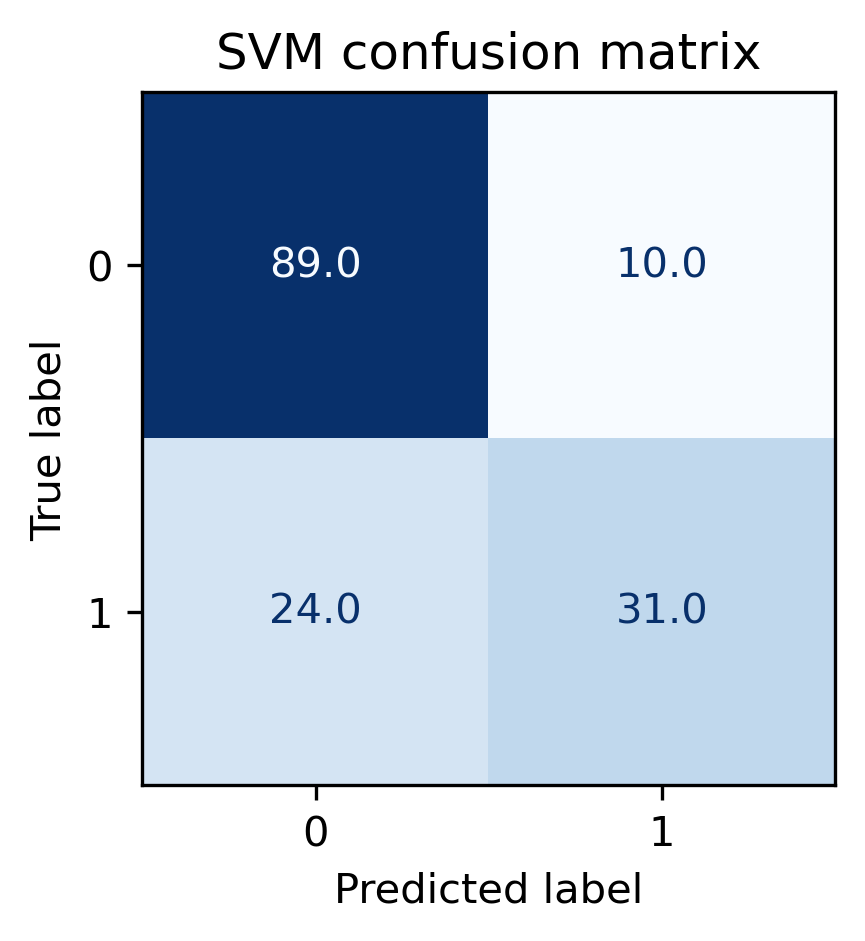
\includegraphics[width=0.5\linewidth]{../HW2_2/SVM confusion.png}}
			\caption{ماتریس سردرگمی برای مدل \lr{Support Vector Machine}}
			\label{fig:confusion_svm}
		\end{figure}
	\pagebreak
	\subsection{جمع‌بندی و مقایسه}
	به صورت خلاصه، نتایج مدل‌های آموزش دیده شده به صورت زیر خواهد بود.
			\begin{table}[h!]
		\caption{جمع‌بندی نتایج مدل‌ها برای پیش‌بینی دیابت}
		\begin{latin}
			\centering
			\begin{tabular}{|l|c|c|}
				\hline
				\textbf{Model} & \textbf{Test precision} & \textbf{Test accuracy} \\ \hline
				Logistic Regression & 0.70454 & 0.75974 \\ \hline
				K Nearest Neighbor & 0.65517 & 0.70129 \\ \hline
				Decision Tree & 0.66666 &  0.74675 \\ \hline
				Random Forest & 0.67272 & 0.76623 \\ \hline
				Support Vector Machine & 0.77922 & 0.75609 \\ \hline
			\end{tabular}
		\end{latin}
		\label{tab:results2} 
		\end{table}
		به طور کلی می‌توان دید که مدل‌های \lr{Logistic Regression} و \lr{SٰVM} با پارامتر‌های بهینه بهترین نتیجه را داشته اند.\\
		در مورد بایاس و واریانس‌های مدل‌های \lr{Decision Tree} و \lr{Random Forest} می‌توان گفت که مدل‌ها درخت تصمیم‌گیری در مرحله تربیت مدل می‌توانند با ساختاری پیچیده داده‌های تربیتی را به خوبی تخمین بزنند. به این ترتیب این مدل در مرحله تربیت از دقت خوبی برخوردار بوده و \underline{بایاس کم} دارد. اما این موضوع به این معناست که این مدل‌ها می‌توانند با افزایش پیچیدگی دچار اورفیت شوند. همچنین واریانس بالایی دارند و تغییرات کوچک در داده‌های آزمون می‌تواند باعث تغییرات بزرگ در پیش‌بینی شود.\\
		از طرفی مدل‌
		\lr{Random Forest}
		یک مدل تجمیعی بوده هر کدام از درخت‌های بایاس پایین دارند اما تجمیع این درخت‌ها باعث بالا رفتن بایاس خواهد شد و نسبت به یک درخت تصمیم‌گیری بایاس بالاتری دارند. اما این افزایش کوچک بایاس نهایتا به همان علت تجمیع چندین درخت، واریانس را در آزمون پایین می‌آورند و مدل تعمیم‌پذیری بهتری خواهد داشت.\\
		جدول زیر نتیجه بایاس و واریانس را برای این دو مدل در این مسئله نشان می‌دهد. در این قسمت بایاس در مدل \lr{Random Forest} تغییر چندانی نکرده است که طبق انتظار باید همینطور بوده یا کمی افزایش پیدا می‌کرد. درباره واریانس طبق انتظار و استدلال قبلی، به صورت قابل توجهی کاهش یافته است.
				\begin{table}[h!]
		\caption{مقایسه بایاس و واریانس مدل‌های \lr{Decision Tree} و \lr{Random Forest}}
		\begin{latin}
			\centering
			\begin{tabular}{|l|c|c|}
				\hline
				\textbf{Model} & \textbf{Bias} & \textbf{Variance} \\ \hline
				Decision Tree & 0.2597 & 0.2223 \\ \hline
				Random Forest & 0.2532 & 0.1057 \\ \hline
			\end{tabular}
		\end{latin}
		\label{tab:results3} 
	\end{table}
	\end{document}